\documentclass[11pt,]{article}
\usepackage{lmodern}
\usepackage{amssymb,amsmath}
\usepackage{ifxetex,ifluatex}
\usepackage{fixltx2e} % provides \textsubscript
\ifnum 0\ifxetex 1\fi\ifluatex 1\fi=0 % if pdftex
  \usepackage[T1]{fontenc}
  \usepackage[utf8]{inputenc}
\else % if luatex or xelatex
  \ifxetex
    \usepackage{mathspec}
  \else
    \usepackage{fontspec}
  \fi
  \defaultfontfeatures{Ligatures=TeX,Scale=MatchLowercase}
\fi
% use upquote if available, for straight quotes in verbatim environments
\IfFileExists{upquote.sty}{\usepackage{upquote}}{}
% use microtype if available
\IfFileExists{microtype.sty}{%
\usepackage{microtype}
\UseMicrotypeSet[protrusion]{basicmath} % disable protrusion for tt fonts
}{}
\usepackage{hyperref}
\hypersetup{unicode=true,
            pdftitle={BSTA 552: Mathematical Statistics II -- Class Notes},
            pdfauthor={Jessica Minnier},
            pdfborder={0 0 0},
            breaklinks=true}
\urlstyle{same}  % don't use monospace font for urls
\usepackage{natbib}
\bibliographystyle{plainnat}
\usepackage{color}
\usepackage{fancyvrb}
\newcommand{\VerbBar}{|}
\newcommand{\VERB}{\Verb[commandchars=\\\{\}]}
\DefineVerbatimEnvironment{Highlighting}{Verbatim}{commandchars=\\\{\}}
% Add ',fontsize=\small' for more characters per line
\usepackage{framed}
\definecolor{shadecolor}{RGB}{248,248,248}
\newenvironment{Shaded}{\begin{snugshade}}{\end{snugshade}}
\newcommand{\AlertTok}[1]{\textcolor[rgb]{0.94,0.16,0.16}{#1}}
\newcommand{\AnnotationTok}[1]{\textcolor[rgb]{0.56,0.35,0.01}{\textbf{\textit{#1}}}}
\newcommand{\AttributeTok}[1]{\textcolor[rgb]{0.77,0.63,0.00}{#1}}
\newcommand{\BaseNTok}[1]{\textcolor[rgb]{0.00,0.00,0.81}{#1}}
\newcommand{\BuiltInTok}[1]{#1}
\newcommand{\CharTok}[1]{\textcolor[rgb]{0.31,0.60,0.02}{#1}}
\newcommand{\CommentTok}[1]{\textcolor[rgb]{0.56,0.35,0.01}{\textit{#1}}}
\newcommand{\CommentVarTok}[1]{\textcolor[rgb]{0.56,0.35,0.01}{\textbf{\textit{#1}}}}
\newcommand{\ConstantTok}[1]{\textcolor[rgb]{0.00,0.00,0.00}{#1}}
\newcommand{\ControlFlowTok}[1]{\textcolor[rgb]{0.13,0.29,0.53}{\textbf{#1}}}
\newcommand{\DataTypeTok}[1]{\textcolor[rgb]{0.13,0.29,0.53}{#1}}
\newcommand{\DecValTok}[1]{\textcolor[rgb]{0.00,0.00,0.81}{#1}}
\newcommand{\DocumentationTok}[1]{\textcolor[rgb]{0.56,0.35,0.01}{\textbf{\textit{#1}}}}
\newcommand{\ErrorTok}[1]{\textcolor[rgb]{0.64,0.00,0.00}{\textbf{#1}}}
\newcommand{\ExtensionTok}[1]{#1}
\newcommand{\FloatTok}[1]{\textcolor[rgb]{0.00,0.00,0.81}{#1}}
\newcommand{\FunctionTok}[1]{\textcolor[rgb]{0.00,0.00,0.00}{#1}}
\newcommand{\ImportTok}[1]{#1}
\newcommand{\InformationTok}[1]{\textcolor[rgb]{0.56,0.35,0.01}{\textbf{\textit{#1}}}}
\newcommand{\KeywordTok}[1]{\textcolor[rgb]{0.13,0.29,0.53}{\textbf{#1}}}
\newcommand{\NormalTok}[1]{#1}
\newcommand{\OperatorTok}[1]{\textcolor[rgb]{0.81,0.36,0.00}{\textbf{#1}}}
\newcommand{\OtherTok}[1]{\textcolor[rgb]{0.56,0.35,0.01}{#1}}
\newcommand{\PreprocessorTok}[1]{\textcolor[rgb]{0.56,0.35,0.01}{\textit{#1}}}
\newcommand{\RegionMarkerTok}[1]{#1}
\newcommand{\SpecialCharTok}[1]{\textcolor[rgb]{0.00,0.00,0.00}{#1}}
\newcommand{\SpecialStringTok}[1]{\textcolor[rgb]{0.31,0.60,0.02}{#1}}
\newcommand{\StringTok}[1]{\textcolor[rgb]{0.31,0.60,0.02}{#1}}
\newcommand{\VariableTok}[1]{\textcolor[rgb]{0.00,0.00,0.00}{#1}}
\newcommand{\VerbatimStringTok}[1]{\textcolor[rgb]{0.31,0.60,0.02}{#1}}
\newcommand{\WarningTok}[1]{\textcolor[rgb]{0.56,0.35,0.01}{\textbf{\textit{#1}}}}
\usepackage{longtable,booktabs}
\usepackage{graphicx,grffile}
\makeatletter
\def\maxwidth{\ifdim\Gin@nat@width>\linewidth\linewidth\else\Gin@nat@width\fi}
\def\maxheight{\ifdim\Gin@nat@height>\textheight\textheight\else\Gin@nat@height\fi}
\makeatother
% Scale images if necessary, so that they will not overflow the page
% margins by default, and it is still possible to overwrite the defaults
% using explicit options in \includegraphics[width, height, ...]{}
\setkeys{Gin}{width=\maxwidth,height=\maxheight,keepaspectratio}
\IfFileExists{parskip.sty}{%
\usepackage{parskip}
}{% else
\setlength{\parindent}{0pt}
\setlength{\parskip}{6pt plus 2pt minus 1pt}
}
\setlength{\emergencystretch}{3em}  % prevent overfull lines
\providecommand{\tightlist}{%
  \setlength{\itemsep}{0pt}\setlength{\parskip}{0pt}}
\setcounter{secnumdepth}{5}
% Redefines (sub)paragraphs to behave more like sections
\ifx\paragraph\undefined\else
\let\oldparagraph\paragraph
\renewcommand{\paragraph}[1]{\oldparagraph{#1}\mbox{}}
\fi
\ifx\subparagraph\undefined\else
\let\oldsubparagraph\subparagraph
\renewcommand{\subparagraph}[1]{\oldsubparagraph{#1}\mbox{}}
\fi

%%% Use protect on footnotes to avoid problems with footnotes in titles
\let\rmarkdownfootnote\footnote%
\def\footnote{\protect\rmarkdownfootnote}

%%% Change title format to be more compact
\usepackage{titling}

% Create subtitle command for use in maketitle
\providecommand{\subtitle}[1]{
  \posttitle{
    \begin{center}\large#1\end{center}
    }
}

\setlength{\droptitle}{-2em}

  \title{BSTA 552: Mathematical Statistics II -- Class Notes}
    \pretitle{\vspace{\droptitle}\centering\huge}
  \posttitle{\par}
    \author{Jessica Minnier}
    \preauthor{\centering\large\emph}
  \postauthor{\par}
      \predate{\centering\large\emph}
  \postdate{\par}
    \date{2019-10-02}




\usepackage{epsfig,latexsym,amsmath, amssymb, amsfonts}
\usepackage{lscape}
\usepackage{paralist}
\usepackage{enumerate}

\usepackage{placeins}
\usepackage{enumitem}
\usepackage[utf8]{inputenc}
\setlist{nolistsep}

\usepackage{epstopdf, graphicx,amsfonts,fullpage,geometry,color,subfigure,eucal,multirow,pdflscape,mathrsfs, latexsym, textcomp}
%\usepackage[pdftex,bookmarks,colorlinks,breaklinks]{hyperref}  % PDF hyperlinks, with coloured links
\definecolor{darkblue}{rgb}{0,0,0.4}
%\hypersetup{linkcolor=black,citecolor=black,filecolor=black,urlcolor=black} % black links, for printed output
\usepackage{memhfixc} 

%
\marginparwidth 0pt
\evensidemargin 0pt
\oddsidemargin 0pt
\marginparsep 0pt
\topmargin 0pt
\textwidth 6.5in
\textheight 8.5in
% next sets eqn skip
\jot=0.4cm
%
%
%for double spacing
  \baselineskip=0.8cm
%
% some commands
%
\newcommand\independent{\protect\mathpalette{\protect\independenT}{\perp}}
\def\independenT#1#2{\mathrel{\rlap{$#1#2$}\mkern2mu{#1#2}}}
%

\newcommand{\Xndots}{X_1, \ldots, X_n}
\newcommand{\LUX}{[L(\bX),U(\bX)]}
\newcommand{\LUx}{[L(\bx),U(\bx)]}

\newcommand{ \Va }{\mbox{\boldmath ${\alpha}$}}
\newcommand{ \Vb }{\mbox{\boldmath ${\beta}$}}
\newcommand{ \Vg }{\mbox{\boldmath ${\gamma}$}}
\newcommand{ \Vt }{\mbox{\boldmath ${\theta}$}}
%\newcommand{ \Vt }{\mbox{\boldmath ${\Theta}$}}
\newcommand{ \wVb }{\widehat{\mbox{\boldmath ${\beta}$}}}
\newcommand{ \wVa }{\widehat{\mbox{\boldmath ${\alpha}$}}}
\newcommand{ \wVt }{\widehat{\mbox{\boldmath ${\theta}$}}}
\newcommand{\var}{{\rm var}\,}
\newcommand{\cov}{{\rm cov}\,}
\newcommand{\bo}[1]{\mbox{\mathversion{bold}$#1$}}
\newenvironment{myitemize}
{ \begin{itemize}
    \setlength{\itemsep}{0pt}
    \setlength{\parskip}{0pt}
    \setlength{\parsep}{0pt}     }
{ \end{itemize}                  } 



\definecolor{blue2}{RGB}{0, 0.245, 0.555}
\definecolor{cyan}{RGB}{024, 055, 155}
\definecolor{pink}{RGB}{255, 105, 180}
\definecolor{red2}{RGB}{200,000,000}
\definecolor{red4}{RGB}{120,000,000}
\definecolor{green}{RGB}{021,122,090}
\definecolor{green4}{RGB}{021,122,090}
\definecolor{green2}{RGB}{000,122,000}
\definecolor{yellow2}{RGB}{180,120,000}
\definecolor{yellow4}{RGB}{120,100,000}
\definecolor{navy}{RGB}{000,000,090}

\newcommand{\smallT}{\scriptscriptstyle{T}}
\newcommand{\ikikp}{ ^{ik}_{\imath \kappa}}
\newcommand{\sumi}{\sum_{i=1}^{n_{\D}}}
\newcommand{\sumip}{\sum_{\imath<i}}
\newcommand{\sumj}{\sum_{j=n_{\D}+1}^{n_{\D}+n_{\C}}}
\newcommand{\suml}{\sum_{l=1}^{K_j}}
\newcommand{\sumk}{\sum_{k=1}^{K_i}}
\newcommand{\sumkp}{\sum_{\kappa=1}^{K_{\imath}}}
\newcommand{\sumik}{\sumi \sumk}
\newcommand{\sumjl}{\sumj \suml}
\newcommand{\nd}{n_{\D}}
\newcommand{\Nd}{N_{\D}}
\newcommand{\nc}{n_{\C}}
\newcommand{\Nc}{N_{\C}}
\newcommand{\ndinv}{\nd^{-1}}
\newcommand{\Ndinv}{\Nd^{-1}}
\newcommand{\ncinv}{\nc^{-1}}
\newcommand{\Ncinv}{\Nc^{-1}}
\newcommand{\nchalf}{\nc^{\half}}
\newcommand{\ncnhalf}{\nc^{-\half}}
\newcommand{\ndhalf}{\nd^{\half}}
\newcommand{\ndnhalf}{\nd^{-\half}}

\newcommand{\Nchalf}{\Nc^{\half}}
\newcommand{\Ncnhalf}{\Nc^{-\half}}
\newcommand{\Ndhalf}{\Nd^{\half}}
\newcommand{\Ndnhalf}{\Nd^{-\half}}
\newcommand{\Ndnq}{\Nd^{-2}}
\newcommand{\Ndnqhalf}{\Nd^{-\frac{3}{2}}}

\newcommand{\md}{m_{\D}}
\newcommand{\mdnqhalf}{\md^{-\frac{3}{2}}}
%
%%%%%%%%%%%%%%%%%%%%%%%%%%
%  Bold Digits           %
%%%%%%%%%%%%%%%%%%%%%%%%%%
%
%
\def\bzero{{\bf 0}}
\def\bone{{\bf 1}}
%
%
%%%%%%%%%%%%%%%%%%%%%%%%%%
%  Bold Roman Letters    %
%%%%%%%%%%%%%%%%%%%%%%%%%%
%
%
\def\ba{{\mbox{\boldmath$a$}}}
\def\bb{{\bf b}}
\def\bc{{\bf c}}
\def\bd{{\bf d}}
\def\be{{\bf e}}
\def\bdf{{\bf f}}
\def\bg{{\mbox{\boldmath$g$}}}
\def\bh{{\bf h}}
\def\bi{{\bf i}}
\def\bj{{\bf j}}
\def\bk{{\bf k}}
\def\bl{{\bf l}}
\def\bm{{\bf m}}
\def\bn{{\bf n}}
\def\bo{{\bf o}}
\def\bp{{\bf p}}
\def\bq{{\bf q}}
\def\br{{\bf r}}
\def\bs{{\bf s}}
\def\bt{{\bf t}}
\def\bu{{\bf u}}
\def\bv{{\bf v}}
\def\bw{{\bf w}}
\def\bx{{\bf x}}
\def\by{{\bf y}}
\def\bz{{\bf z}}
\def\bA{{\bf A}}
\def\bB{{\bf B}}
\def\bC{{\bf C}}
\def\bD{{\bf D}}
\def\bE{{\bf E}}
\def\bF{{\bf F}}
\def\bG{{\bf G}}
\def\bH{{\bf H}}
\def\bI{{\bf I}}
\def\bJ{{\bf J}}
\def\bK{{\bf K}}
\def\bL{{\bf L}}
\def\bM{{\bf M}}
\def\bN{{\bf N}}
\def\bO{{\bf O}}
\def\bP{{\bf P}}
\def\bQ{{\bf Q}}
\def\bR{{\bf R}}
\def\bS{{\bf S}}
\def\bT{{\bf T}}
\def\bU{{\bf U}}
\def\bV{{\bf V}}
\def\bW{{\bf W}}
\def\bX{{\bf X}}
\def\bY{{\bf Y}}
\def\bZ{{\bf Z}}
\def\smbZ{\scriptstyle{\bf Z}}
\def\smM{\scriptstyle{M}}
\def\smN{\scriptstyle{N}}
\def\smbT{\scriptstyle{\bf T}}
%
%
%%%%%%%%%%%%%%%%%%%%%%%%%%
%  Bold Greek Letters    %
%%%%%%%%%%%%%%%%%%%%%%%%%%
%
%
\def\thick#1{\hbox{\rlap{$#1$}\kern0.25pt\rlap{$#1$}\kern0.25pt$#1$}}
\def\balpha{\boldsymbol{\alpha}}
\def\bbeta{\boldsymbol{\beta}}
\def\bgamma{\boldsymbol{\gamma}}
\def\bdelta{\boldsymbol{\delta}}
\def\bepsilon{\boldsymbol{\epsilon}}
\def\bvarepsilon{\boldsymbol{\varepsilon}}
\def\bzeta{\boldsymbol{\zeta}}
\def\bdeta{\boldsymbol{\eta}}
\def\btheta{\boldsymbol{\theta}}
\def\biota{\boldsymbol{\iota}}
\def\bkappa{\boldsymbol{\kappa}}
\def\blambda{\boldsymbol{\lambda}}
\def\bmu{\boldsymbol{\mu}}
\def\bnu{\boldsymbol{\nu}}
\def\bxi{\boldsymbol{\xi}}
\def\bomicron{\boldsymbol{\omicron}}
\def\bpi{\boldsymbol{\pi}}
\def\brho{\boldsymbol{\rho}}
\def\bsigma{\boldsymbol{\sigma}}
\def\btau{\boldsymbol{\tau}}
\def\bupsilon{\boldsymbol{\upsilon}}
\def\bphi{\boldsymbol{\phi}}
\def\bchi{\boldsymbol{\chi}}
\def\bpsi{\boldsymbol{\psi}}
\def\bomega{\boldsymbol{\omega}}
\def\bAlpha{\boldsymbol{\Alpha}}
\def\bBeta{\boldsymbol{\Beta}}
\def\bGamma{\boldsymbol{\Gamma}}
\def\bDelta{\boldsymbol{\Delta}}
\def\bEpsilon{\boldsymbol{\Epsilon}}
\def\bZeta{\boldsymbol{\Zeta}}
\def\bEta{\boldsymbol{\Eta}}
\def\bTheta{\boldsymbol{\Theta}}
\def\bIota{\boldsymbol{\Iota}}
\def\bKappa{\boldsymbol{\Kappa}}
\def\bLambda{{\boldsymbol{\Lambda}}}
\def\bMu{\boldsymbol{\Mu}}
\def\bNu{\boldsymbol{\Nu}}
\def\bXi{\boldsymbol{\Xi}}
\def\bOmicron{\boldsymbol{\Omicron}}
\def\bPi{\boldsymbol{\Pi}}
\def\bRho{\boldsymbol{\Rho}}
\def\bSigma{\boldsymbol{\Sigma}}
\def\bTau{\boldsymbol{\Tau}}
\def\bUpsilon{\boldsymbol{\Upsilon}}
\def\bPhi{\boldsymbol{\Phi}}
\def\bChi{\boldsymbol{\Chi}}
\def\bPsi{\boldsymbol{\Psi}}
\def\bOmega{\boldsymbol{\Omega}}
%
%
%
%%%%%%%%%%%%%%%%%%%%%%%%%%%%%%%%
%  Small Bold Greek Letters    %
%%%%%%%%%%%%%%%%%%%%%%%%%%%%%%%%
\def\smalpha{{{\scriptstyle{\alpha}}}}
\def\smbeta{{{\scriptstyle{\beta}}}}
\def\smgamma{{{\scriptstyle{\gamma}}}}
\def\smdelta{{{\scriptstyle{\delta}}}}
\def\smepsilon{{{\scriptstyle{\epsilon}}}}
\def\smvarepsilon{{{\scriptstyle{\varepsilon}}}}
\def\smzeta{{{\scriptstyle{\zeta}}}}
\def\smdeta{{{\scriptstyle{\eta}}}}
\def\smtheta{{{\scriptstyle{\theta}}}}
\def\smiota{{{\scriptstyle{\iota}}}}
\def\smkappa{{{\scriptstyle{\kappa}}}}
\def\smlambda{{{\scriptstyle{\lambda}}}}
\def\smmu{{{\scriptstyle{\mu}}}}
\def\smnu{{{\scriptstyle{\nu}}}}
\def\smxi{{{\scriptstyle{\xi}}}}
\def\smomicron{{{\scriptstyle{\omicron}}}}
\def\smpi{{{\scriptstyle{\pi}}}}
\def\smrho{{{\scriptstyle{\rho}}}}
\def\smsigma{{{\scriptstyle{\sigma}}}}
\def\smtau{{{\scriptstyle{\tau}}}}
\def\smupsilon{{{\scriptstyle{\upsilon}}}}
\def\smphi{{{\scriptstyle{\phi}}}}
\def\smchi{{{\scriptstyle{\chi}}}}
\def\smpsi{{{\scriptstyle{\psi}}}}
\def\smomega{{{\scriptstyle{\omega}}}}
\def\smAlpha{{{\scriptstyle{\Alpha}}}}
\def\smBeta{{{\scriptstyle{\Beta}}}}
\def\smGamma{{{\scriptstyle{\Gamma}}}}
\def\smDelta{{{\scriptstyle{\Delta}}}}
\def\smEpsilon{{{\scriptstyle{\Epsilon}}}}
\def\smZeta{{{\scriptstyle{\Zeta}}}}
\def\smEta{{{\scriptstyle{\Eta}}}}
\def\smTheta{{{\scriptstyle{\Theta}}}}
\def\smIota{{{\scriptstyle{\Iota}}}}
\def\smKappa{{{\scriptstyle{\Kappa}}}}
\def\smLambda{{{\scriptstyle{\Lambda}}}}
\def\smMu{{{\scriptstyle{\Mu}}}}
\def\smNu{{{\scriptstyle{\Nu}}}}
\def\smXi{{{\scriptstyle{\Xi}}}}
\def\smOmicron{{{\scriptstyle{\Omicron}}}}
\def\smPi{{{\scriptstyle{\Pi}}}}
\def\smRho{{{\scriptstyle{\Rho}}}}
\def\smSigma{{{\scriptstyle{\Sigma}}}}
\def\smTau{{{\scriptstyle{\Tau}}}}
\def\smUpsilon{{{\scriptstyle{\Upsilon}}}}
\def\smPhi{{{\scriptstyle{\Phi}}}}
\def\smChi{{{\scriptstyle{\Chi}}}}
\def\smPsi{{{\scriptstyle{\Psi}}}}
\def\smOmega{{{\scriptstyle{\Omega}}}}
%
%

%
%%%%%%%%%%%%%%%%%%%%%%%%%%%%%%%%
%  Small Bold Greek Letters    %
%%%%%%%%%%%%%%%%%%%%%%%%%%%%%%%%
\def\smbalpha{\boldsymbol{{\scriptstyle{\alpha}}}}
\def\smbbeta{\boldsymbol{{\scriptstyle{\beta}}}}
\def\smbgamma{\boldsymbol{{\scriptstyle{\gamma}}}}
\def\smbdelta{\boldsymbol{{\scriptstyle{\delta}}}}
\def\smbepsilon{\boldsymbol{{\scriptstyle{\epsilon}}}}
\def\smbvarepsilon{\boldsymbol{{\scriptstyle{\varepsilon}}}}
\def\smbzeta{\boldsymbol{{\scriptstyle{\zeta}}}}
\def\smbdeta{\boldsymbol{{\scriptstyle{\eta}}}}
\def\smbtheta{\boldsymbol{{\scriptstyle{\theta}}}}
\def\smbiota{\boldsymbol{{\scriptstyle{\iota}}}}
\def\smbkappa{\boldsymbol{{\scriptstyle{\kappa}}}}
\def\smblambda{\boldsymbol{{\scriptstyle{\lambda}}}}
\def\smbmu{\boldsymbol{{\scriptstyle{\mu}}}}
\def\smbnu{\boldsymbol{{\scriptstyle{\nu}}}}
\def\smbxi{\boldsymbol{{\scriptstyle{\xi}}}}
\def\smbomicron{\boldsymbol{{\scriptstyle{\omicron}}}}
\def\smbpi{\boldsymbol{{\scriptstyle{\pi}}}}
\def\smbrho{\boldsymbol{{\scriptstyle{\rho}}}}
\def\smbsigma{\boldsymbol{{\scriptstyle{\sigma}}}}
\def\smbtau{\boldsymbol{{\scriptstyle{\tau}}}}
\def\smbupsilon{\boldsymbol{{\scriptstyle{\upsilon}}}}
\def\smbphi{\boldsymbol{{\scriptstyle{\phi}}}}
\def\smbchi{\boldsymbol{{\scriptstyle{\chi}}}}
\def\smbpsi{\boldsymbol{{\scriptstyle{\psi}}}}
\def\smbomega{\boldsymbol{{\scriptstyle{\omega}}}}
\def\smbAlpha{\boldsymbol{{\scriptstyle{\Alpha}}}}
\def\smbBeta{\boldsymbol{{\scriptstyle{\Beta}}}}
\def\smbGamma{\boldsymbol{{\scriptstyle{\Gamma}}}}
\def\smbDelta{\boldsymbol{{\scriptstyle{\Delta}}}}
\def\smbEpsilon{\boldsymbol{{\scriptstyle{\Epsilon}}}}
\def\smbZeta{\boldsymbol{{\scriptstyle{\Zeta}}}}
\def\smbEta{\boldsymbol{{\scriptstyle{\Eta}}}}
\def\smbTheta{\boldsymbol{{\scriptstyle{\Theta}}}}
\def\smbIota{\boldsymbol{{\scriptstyle{\Iota}}}}
\def\smbKappa{\boldsymbol{{\scriptstyle{\Kappa}}}}
\def\smbLambda{\boldsymbol{{\scriptstyle{\Lambda}}}}
\def\smbMu{\boldsymbol{{\scriptstyle{\Mu}}}}
\def\smbNu{\boldsymbol{{\scriptstyle{\Nu}}}}
\def\smbXi{\boldsymbol{{\scriptstyle{\Xi}}}}
\def\smbOmicron{\boldsymbol{{\scriptstyle{\Omicron}}}}
\def\smbPi{\boldsymbol{{\scriptstyle{\Pi}}}}
\def\smbRho{\boldsymbol{{\scriptstyle{\Rho}}}}
\def\smbSigma{\boldsymbol{{\scriptstyle{\Sigma}}}}
\def\smbTau{\boldsymbol{{\scriptstyle{\Tau}}}}
\def\smbUpsilon{\boldsymbol{{\scriptstyle{\Upsilon}}}}
\def\smbPhi{\boldsymbol{{\scriptstyle{\Phi}}}}
\def\smbChi{\boldsymbol{{\scriptstyle{\Chi}}}}
\def\smbPsi{\boldsymbol{{\scriptstyle{\Psi}}}}
\def\smbOmega{\boldsymbol{{\scriptstyle{\Omega}}}}
%
%
%%%%%%%%%%%%%%%%%%%%%%%%%%
%  Hatted Roman Letters  %
%%%%%%%%%%%%%%%%%%%%%%%%%%
%
%
\def\ahat{{\widehat a}}
\def\bhat{{\widehat b}}
\def\chat{{\widehat c}}
\def\dhat{{\widehat d}}
\def\ehat{{\widehat e}}
\def\fhat{{\widehat f}}
\def\ghat{{\widehat g}}
\def\hhat{{\widehat h}}
\def\ihat{{\widehat i}}
\def\jhat{{\widehat j}}
\def\khat{{\widehat k}}
\def\lhat{{\widehat l}}
\def\mhat{{\widehat m}}
\def\nhat{{\widehat n}}
\def\ohat{{\widehat o}}
\def\phat{{\widehat p}}
\def\qhat{{\widehat q}}
\def\rhat{{\widehat r}}
\def\shat{{\widehat s}}
\def\that{{\widehat t}}
\def\uhat{{\widehat u}}
\def\vhat{{\widehat v}}
\def\what{{\widehat w}}
\def\xhat{{\widehat x}}
\def\yhat{{\widehat y}}
\def\zhat{{\widehat z}}
\def\Ahat{{\widehat A}}
\def\Bhat{{\widehat B}}
\def\Chat{{\widehat C}}
\def\Dhat{{\widehat D}}
\def\Ehat{{\widehat E}}
\def\Fhat{{\widehat F}}
\def\Ghat{{\widehat G}}
\def\Hhat{{\widehat H}}
\def\Ihat{{\widehat I}}
\def\Jhat{{\widehat J}}
\def\Khat{{\widehat K}}
\def\Lhat{{\widehat L}}
\def\Mhat{{\widehat M}}
\def\Nhat{{\widehat N}}
\def\Ohat{{\widehat O}}
\def\Phat{{\widehat P}}
\def\Qhat{{\widehat Q}}
\def\Rhat{{\widehat R}}
\def\Shat{{\widehat S}}
\def\That{{\widehat T}}
\def\Uhat{{\widehat U}}
\def\Vhat{{\widehat V}}
\def\What{{\widehat W}}
\def\Xhat{{\widehat X}}
\def\Yhat{{\widehat Y}}
\def\Zhat{{\widehat Z}}
%
%%%%%%%%%%%%%%%%%%%%%%%%%%
%  Tilded Roman Letters  %
%%%%%%%%%%%%%%%%%%%%%%%%%%
%
%
\def\atilde{{\widetilde a}}
\def\btilde{{\widetilde b}}
\def\ctilde{{\widetilde c}}
\def\dtilde{{\widetilde d}}
\def\etilde{{\widetilde e}}
\def\ftilde{{\widetilde f}}
\def\gtilde{{\widetilde g}}
\def\htilde{{\widetilde h}}
\def\itilde{{\widetilde i}}
\def\jtilde{{\widetilde j}}
\def\ktilde{{\widetilde k}}
\def\ltilde{{\widetilde l}}
\def\mtilde{{\widetilde m}}
\def\ntilde{{\widetilde n}}
\def\otilde{{\widetilde o}}
\def\ptilde{{\widetilde p}}
\def\qtilde{{\widetilde q}}
\def\rtilde{{\widetilde r}}
\def\stilde{{\widetilde s}}
\def\ttilde{{\widetilde t}}
\def\utilde{{\widetilde u}}
\def\vtilde{{\widetilde v}}
\def\wtilde{{\widetilde w}}
\def\xtilde{{\widetilde x}}
\def\ytilde{{\widetilde y}}
\def\ztilde{{\widetilde z}}
\def\Atilde{{\widetilde A}}
\def\Btilde{{\widetilde B}}
\def\Ctilde{{\widetilde C}}
\def\Dtilde{{\widetilde D}}
\def\Etilde{{\widetilde E}}
\def\Ftilde{{\widetilde F}}
\def\Gtilde{{\widetilde G}}
\def\Htilde{{\widetilde H}}
\def\Itilde{{\widetilde I}}
\def\Jtilde{{\widetilde J}}
\def\Ktilde{{\widetilde K}}
\def\Ltilde{{\widetilde L}}
\def\Mtilde{{\widetilde M}}
\def\Ntilde{{\widetilde N}}
\def\Otilde{{\widetilde O}}
\def\Ptilde{{\widetilde P}}
\def\Qtilde{{\widetilde Q}}
\def\Rtilde{{\widetilde R}}
\def\Stilde{{\widetilde S}}
\def\Ttilde{{\widetilde T}}
\def\Utilde{{\widetilde U}}
\def\Vtilde{{\widetilde V}}
\def\Wtilde{{\widetilde W}}
\def\Xtilde{{\widetilde X}}
\def\Ytilde{{\widetilde Y}}
\def\Ztilde{{\widetilde Z}}
%
%
%%%%%%%%%%%%%%%%%%%%%%%%%%%%%%%%%%%%
%  Hatted Bold-faced Roman Letters %
%%%%%%%%%%%%%%%%%%%%%%%%%%%%%%%%%%%%
%
%
\def\bahat{{\widehat \ba}}
\def\bbhat{{\widehat \bb}}
\def\bchat{{\widehat \bc}}
\def\bdhat{{\widehat \bd}}
\def\behat{{\widehat \be}}
\def\bfhat{{\widehat \bf}}
\def\bghat{{\widehat \bg}}
\def\bhhat{{\widehat \bh}}
\def\bihat{{\widehat \bi}}
\def\bjhat{{\widehat \bj}}
\def\bkhat{{\widehat \bk}}
\def\blhat{{\widehat \bl}}
\def\bmhat{{\widehat \bm}}
\def\bnhat{{\widehat \bn}}
\def\bohat{{\widehat \bo}}
\def\bphat{{\widehat \bp}}
\def\bqhat{{\widehat \bq}}
\def\brhat{{\widehat \br}}
\def\bshat{{\widehat \bs}}
\def\bthat{{\widehat \bt}}
\def\buhat{{\widehat \bu}}
\def\bvhat{{\widehat \bv}}
\def\bwhat{{\widehat \bw}}
\def\bxhat{{\widehat \bx}}
\def\byhat{{\widehat \by}}
\def\bzhat{{\widehat \bz}}
\def\bAhat{{\widehat \bA}}
\def\bBhat{{\widehat \bB}}
\def\bChat{{\widehat \bC}}
\def\bDhat{{\widehat \bD}}
\def\bEhat{{\widehat \bE}}
\def\bFhat{{\widehat \bF}}
\def\bGhat{{\widehat \bG}}
\def\bHhat{{\widehat \bH}}
\def\bIhat{{\widehat \bI}}
\def\bJhat{{\widehat \bJ}}
\def\bKhat{{\widehat \bK}}
\def\bLhat{{\widehat \bL}}
\def\bMhat{{\widehat \bM}}
\def\bNhat{{\widehat \bN}}
\def\bOhat{{\widehat \bO}}
\def\bPhat{{\widehat \bP}}
\def\bQhat{{\widehat \bQ}}
\def\bRhat{{\widehat \bR}}
\def\bShat{{\widehat \bS}}
\def\bThat{{\widehat \bT}}
\def\bUhat{{\widehat \bU}}
\def\bVhat{{\widehat \bV}}
\def\bWhat{{\widehat \bW}}
\def\bXhat{{\widehat \bX}}
\def\bYhat{{\widehat \bY}}
\def\bZhat{{\widehat \bZ}}
%
%
%
%%%%%%%%%%%%%%%%%%%%%%%%%%%%%%%%%%%%
%  Tilded Bold-faced Roman Letters %
%%%%%%%%%%%%%%%%%%%%%%%%%%%%%%%%%%%%
%
%
\def\batilde{{\widetilde \ba}}
\def\bbtilde{{\widetilde \bb}}
\def\bctilde{{\widetilde \bc}}
\def\bdtilde{{\widetilde \bd}}
\def\betilde{{\widetilde \be}}
\def\bftilde{{\widetilde \bf}}
\def\bgtilde{{\widetilde \bg}}
\def\bhtilde{{\widetilde \bh}}
\def\bitilde{{\widetilde \bi}}
\def\bjtilde{{\widetilde \bj}}
\def\bktilde{{\widetilde \bk}}
\def\bltilde{{\widetilde \bl}}
\def\bmtilde{{\widetilde \bm}}
\def\bntilde{{\widetilde \bn}}
\def\botilde{{\widetilde \bo}}
\def\bptilde{{\widetilde \bp}}
\def\bqtilde{{\widetilde \bq}}
\def\brtilde{{\widetilde \br}}
\def\bstilde{{\widetilde \bs}}
\def\bttilde{{\widetilde \bt}}
\def\butilde{{\widetilde \bu}}
\def\bvtilde{{\widetilde \bv}}
\def\bwtilde{{\widetilde \bw}}
\def\bxtilde{{\widetilde \bx}}
\def\bytilde{{\widetilde \by}}
\def\bztilde{{\widetilde \bz}}
\def\bAtilde{{\widetilde \bA}}
\def\bBtilde{{\widetilde \bB}}
\def\bCtilde{{\widetilde \bC}}
\def\bDtilde{{\widetilde \bD}}
\def\bEtilde{{\widetilde \bE}}
\def\bFtilde{{\widetilde \bF}}
\def\bGtilde{{\widetilde \bG}}
\def\bHtilde{{\widetilde \bH}}
\def\bItilde{{\widetilde \bI}}
\def\bJtilde{{\widetilde \bJ}}
\def\bKtilde{{\widetilde \bK}}
\def\bLtilde{{\widetilde \bL}}
\def\bMtilde{{\widetilde \bM}}
\def\bNtilde{{\widetilde \bN}}
\def\bOtilde{{\widetilde \bO}}
\def\bPtilde{{\widetilde \bP}}
\def\bQtilde{{\widetilde \bQ}}
\def\bRtilde{{\widetilde \bR}}
\def\bStilde{{\widetilde \bS}}
\def\bTtilde{{\widetilde \bT}}
\def\bUtilde{{\widetilde \bU}}
\def\bVtilde{{\widetilde \bV}}
\def\bWtilde{{\widetilde \bW}}
\def\bXtilde{{\widetilde \bX}}
\def\bYtilde{{\widetilde \bY}}
\def\bZtilde{{\widetilde \bZ}}
%
%
%
%
%%%%%%%%%%%%%%%%%%%%%%%%%%
%  Hatted Greek Letters  %
%%%%%%%%%%%%%%%%%%%%%%%%%%
%
%
\def\alphahat{{\widehat\alpha}}
\def\betahat{{\widehat\beta}}
\def\gammahat{{\widehat\gamma}}
\def\deltahat{{\widehat\delta}}
\def\epsilonhat{{\widehat\epsilon}}
\def\varepsilonhat{{\widehat\varepsilon}}
\def\zetahat{{\widehat\zeta}}
\def\etahat{{\widehat\eta}}
\def\thetahat{{\widehat\theta}}
\def\iotahat{{\widehat\iota}}
\def\kappahat{{\widehat\kappa}}
\def\lambdahat{{\widehat\lambda}}
\def\muhat{{\widehat\mu}}
\def\nuhat{{\widehat\nu}}
\def\xihat{{\widehat\xi}}
\def\omicronhat{{\widehat\omicron}}
\def\pihat{{\widehat\pi}}
\def\rhohat{{\widehat\rho}}
\def\sigmahat{{\widehat\sigma}}
\def\tauhat{{\widehat\tau}}
\def\upsilonhat{{\widehat\upsilon}}
\def\phihat{{\widehat\phi}}
\def\chihat{{\widehat\chi}}
\def\psihat{{\widehat\psi}}
\def\omegahat{{\widehat\omega}}
\def\Alphahat{{\widehat\Alpha}}
\def\Betahat{{\widehat\Beta}}
\def\Gammahat{{\widehat\Gamma}}
\def\Deltahat{{\widehat\Delta}}
\def\Epsilonhat{{\widehat\Epsilon}}
\def\Zetahat{{\widehat\Zeta}}
\def\Etahat{{\widehat\Eta}}
\def\Thetahat{{\widehat\Theta}}
\def\Iotahat{{\widehat\Iota}}
\def\Kappahat{{\widehat\Kappa}}
\def\Lambdahat{{\widehat\Lambda}}
\def\Muhat{{\widehat\Mu}}
\def\Nuhat{{\widehat\Nu}}
\def\Xihat{{\widehat\Xi}}
\def\Omicronhat{{\widehat\Omicron}}
\def\Pihat{{\widehat\Pi}}
\def\Rhohat{{\widehat\Rho}}
\def\Sigmahat{{\widehat\Sigma}}
\def\Tauhat{{\widehat\Tau}}
\def\Upsilonhat{{\widehat\Upsilon}}
\def\Phihat{{\widehat\Phi}}
\def\Chihat{{\widehat\Chi}}
\def\Psihat{{\widehat\Psi}}
\def\Omegahat{{\widehat\Omega}}
%
%
%
%%%%%%%%%%%%%%%%%%%%%%%%%%
%  Tilded Greek Letters  %
%%%%%%%%%%%%%%%%%%%%%%%%%%
%
%
\def\alphatilde{{\widetilde\alpha}}
\def\betatilde{{\widetilde\beta}}
\def\gammatilde{{\widetilde\gamma}}
\def\deltatilde{{\widetilde\delta}}
\def\epsilontilde{{\widetilde\epsilon}}
\def\varepsilontilde{{\widetilde\varepsilon}}
\def\zetatilde{{\widetilde\zeta}}
\def\etatilde{{\widetilde\eta}}
\def\thetatilde{{\widetilde\theta}}
\def\iotatilde{{\widetilde\iota}}
\def\kappatilde{{\widetilde\kappa}}
\def\lambdatilde{{\widetilde\lambda}}
\def\mutilde{{\widetilde\mu}}
\def\nutilde{{\widetilde\nu}}
\def\xitilde{{\widetilde\xi}}
\def\omicrontilde{{\widetilde\omicron}}
\def\pitilde{{\widetilde\pi}}
\def\rhotilde{{\widetilde\rho}}
\def\sigmatilde{{\widetilde\sigma}}
\def\tautilde{{\widetilde\tau}}
\def\upsilontilde{{\widetilde\upsilon}}
\def\phitilde{{\widetilde\phi}}
\def\chitilde{{\widetilde\chi}}
\def\psitilde{{\widetilde\psi}}
\def\omegatilde{{\widetilde\omega}}
\def\Alphatilde{{\widetilde\Alpha}}
\def\Betatilde{{\widetilde\Beta}}
\def\Gammatilde{{\widetilde\Gamma}}
\def\Deltatilde{{\widetilde\Delta}}
\def\Epsilontilde{{\widetilde\Epsilon}}
\def\Zetatilde{{\widetilde\Zeta}}
\def\Etatilde{{\widetilde\Eta}}
\def\Thetatilde{{\widetilde\Theta}}
\def\Iotatilde{{\widetilde\Iota}}
\def\Kappatilde{{\widetilde\Kappa}}
\def\Lambdatilde{{\widetilde\Lambda}}
\def\Mutilde{{\widetilde\Mu}}
\def\Nutilde{{\widetilde\Nu}}
\def\Xitilde{{\widetilde\Xi}}
\def\Omicrontilde{{\widetilde\Omicron}}
\def\Pitilde{{\widetilde\Pi}}
\def\Rhotilde{{\widetilde\Rho}}
\def\Sigmatilde{{\widetilde\Sigma}}
\def\Tautilde{{\widetilde\Tau}}
\def\Upsilontilde{{\widetilde\Upsilon}}
\def\Phitilde{{\widetilde\Phi}}
\def\Chitilde{{\widetilde\Chi}}
\def\Psitilde{{\widetilde\Psi}}
\def\Omegatilde{{\widetilde\Omega}}
%
%
%
%
%%%%%%%%%%%%%%%%%%%%%%%%%%%%%%%%%%%%%
%  Hatted Bold-faced Greek Letters  %
%%%%%%%%%%%%%%%%%%%%%%%%%%%%%%%%%%%%%
%
%
\def\balphahat{{\widehat\balpha}}
\def\bbetahat{{\widehat\bbeta}}
\def\bgammahat{{\widehat\bgamma}}
\def\bdeltahat{{\widehat\bdelta}}
\def\bepsilonhat{{\widehat\bepsilon}}
\def\bzetahat{{\widehat\bzeta}}
\def\bdetahat{{\widehat\bdeta}}
\def\bthetahat{{\widehat\btheta}}
\def\biotahat{{\widehat\biota}}
\def\bkappahat{{\widehat\bkappa}}
\def\blambdahat{{\widehat\blambda}}
\def\bmuhat{{\widehat\bmu}}
\def\bnuhat{{\widehat\bnu}}
\def\bxihat{{\widehat\bxi}}
\def\bomicronhat{{\widehat\bomicron}}
\def\bpihat{{\widehat\bpi}}
\def\brhohat{{\widehat\brho}}
\def\bsigmahat{{\widehat\bsigma}}
\def\btauhat{{\widehat\btau}}
\def\bupsilonhat{{\widehat\bupsilon}}
\def\bphihat{{\widehat\bphi}}
\def\bchihat{{\widehat\bchi}}
\def\bpsihat{{\widehat\bpsi}}
\def\bomegahat{{\widehat\bomega}}
\def\bAlphahat{{\widehat\bAlpha}}
\def\bBetahat{{\widehat\bBeta}}
\def\bGammahat{{\widehat\bGamma}}
\def\bDeltahat{{\widehat\bDelta}}
\def\bEpsilonhat{{\widehat\bEpsilon}}
\def\bZetahat{{\widehat\bZeta}}
\def\bEtahat{{\widehat\bEta}}
\def\bThetahat{{\widehat\bTheta}}
\def\bIotahat{{\widehat\bIota}}
\def\bKappahat{{\widehat\bKappa}}
\def\bLambdahat{{\widehat\bLambda}}
\def\bMuhat{{\widehat\bMu}}
\def\bNuhat{{\widehat\bNu}}
\def\bXihat{{\widehat\bXi}}
\def\bOmicronhat{{\widehat\bOmicron}}
\def\bPihat{{\widehat\bPi}}
\def\bRhohat{{\widehat\bRho}}
\def\bSigmahat{{\widehat\bSigma}}
\def\bTauhat{{\widehat\bTau}}
\def\bUpsilonhat{{\widehat\bUpsilon}}
\def\bPhihat{{\widehat\bPhi}}
\def\bChihat{{\widehat\bChi}}
\def\bPsihat{{\widehat\bPsi}}
\def\bOmegahat{{\widehat\bOmega}}%
%
%
\def\balphahattrans{{\balphahat^{_{\transpose}}}}
\def\bbetahattrans{{\bbetahat^{_{\transpose}}}}
\def\bgammahattrans{{\bgammahat^{_{\transpose}}}}
\def\bdeltahattrans{{\bdeltahat^{_{\transpose}}}}
\def\bepsilonhattrans{{\bepsilonhat^{_{\transpose}}}}
\def\bzetahattrans{{\bzetahat^{_{\transpose}}}}
\def\bdetahattrans{{\bdetahat^{_{\transpose}}}}
\def\bthetahattrans{{\bthetahat^{_{\transpose}}}}
\def\biotahattrans{{\biotahat^{_{\transpose}}}}
\def\bkappahattrans{{\bkappahat^{_{\transpose}}}}
\def\blambdahattrans{{\blambdahat^{_{\transpose}}}}
\def\bmuhattrans{{\bmuhat^{_{\transpose}}}}
\def\bnuhattrans{{\bnuhat^{_{\transpose}}}}
\def\bxihattrans{{\bxihat^{_{\transpose}}}}
\def\bomicronhattrans{{\bomicronhat^{_{\transpose}}}}
\def\bpihattrans{{\bpihat^{_{\transpose}}}}
\def\brhohattrans{{\brhohat^{_{\transpose}}}}
\def\bsigmahattrans{{\bsigmahat^{_{\transpose}}}}
\def\btauhattrans{{\btauhat^{_{\transpose}}}}
\def\bupsilonhattrans{{\bupsilonhat^{_{\transpose}}}}
\def\bphihattrans{{\bphihat^{_{\transpose}}}}
\def\bchihattrans{{\bchihat^{_{\transpose}}}}
\def\bpsihattrans{{\bpsihat^{_{\transpose}}}}
\def\bomegahattrans{{\bomegahat^{_{\transpose}}}}
\def\bAlphahattrans{{\bAlphahat^{_{\transpose}}}}
\def\bBetahattrans{{\bBetahat^{_{\transpose}}}}
\def\bGammahattrans{{\bGammahat^{_{\transpose}}}}
\def\bDeltahattrans{{\bDeltahat^{_{\transpose}}}}
\def\bEpsilonhattrans{{\bEpsilonhat^{_{\transpose}}}}
\def\bZetahattrans{{\bZetahat^{_{\transpose}}}}
\def\bEtahattrans{{\bEtahat^{_{\transpose}}}}
\def\bThetahattrans{{\bThetahat^{_{\transpose}}}}
\def\bIotahattrans{{\bIotahat^{_{\transpose}}}}
\def\bKappahattrans{{\bKappahat^{_{\transpose}}}}
\def\bLambdahattrans{{\bLambdahat^{_{\transpose}}}}
\def\bMuhattrans{{\bMuhat^{_{\transpose}}}}
\def\bNuhattrans{{\bNuhat^{_{\transpose}}}}
\def\bXihattrans{{\bXihat^{_{\transpose}}}}
\def\bOmicronhattrans{{\bOmicronhat^{_{\transpose}}}}
\def\bPihattrans{{\bPihat^{_{\transpose}}}}
\def\bRhohattrans{{\bRhohat^{_{\transpose}}}}
\def\bSigmahattrans{{\bSigmahat^{_{\transpose}}}}
\def\bTauhattrans{{\bTauhat^{_{\transpose}}}}
\def\bUpsilonhattrans{{\bUpsilonhat^{_{\transpose}}}}
\def\bPhihattrans{{\bPhihat^{_{\transpose}}}}
\def\bChihattrans{{\bChihat^{_{\transpose}}}}
\def\bPsihattrans{{\bPsihat^{_{\transpose}}}}
\def\bOmegahattrans{{\bOmegahat^{_{\transpose}}}}%
%
%%%%%%%%%%%%%%%%%%%%%%%%%%%%%%%%%%%%%%%
%  Hatted Small Bold Greek Letters    %
%%%%%%%%%%%%%%%%%%%%%%%%%%%%%%%%%%%%%%%
\def\smbalpha{\widehat{\smbalpha}}
\def\smbbetahat{\widehat{\smbbeta}}
\def\smbgammahat{\widehat{\smbgamma}}
\def\smbdeltahat{\widehat{\smbdelta}}
\def\smbepsilonhat{\widehat{\smbepsilon}}
\def\smbvarepsilonhat{\widehat{\smbvarepsilon}}
\def\smbzetahat{\widehat{\smbzeta}}
\def\smbdetahat{\widehat{\smbeta}}
\def\smbthetahat{\widehat{\smbtheta}}
\def\smbiotahat{\widehat{\smbiota}}
\def\smbkappahat{\widehat{\smbkappa}}
\def\smblambdahat{\widehat{\smblambda}}
\def\smbmuhat{\widehat{\smbmu}}
\def\smbnuhat{\widehat{\smbnu}}
\def\smbxihat{\widehat{\smbxi}}
\def\smbomicronhat{\widehat{\smbomicron}}
\def\smbpihat{\widehat{\smbpi}}
\def\smbrhohat{\widehat{\smbrho}}
\def\smbsigmahat{\widehat{\smbsigma}}
\def\smbtauhat{\widehat{\smbtau}}
\def\smbupsilonhat{\widehat{\smbupsilon}}
\def\smbphihat{\widehat{\smbphi}}
\def\smbchihat{\widehat{\smbchi}}
\def\smbpsihat{\widehat{\smbpsi}}
\def\smbomegahat{\widehat{\smbomega}}
\def\smbAlphahat{\widehat{\smbAlpha}}
\def\smbBetahat{\widehat{\smbBeta}}
\def\smbGammahat{\widehat{\smbGamma}}
\def\smbDeltahat{\widehat{\smbDelta}}
\def\smbEpsilonhat{\widehat{\smbEpsilon}}
\def\smbZetahat{\widehat{\smbZeta}}
\def\smbEtahat{\widehat{\smbEta}}
\def\smbThetahat{\widehat{\smbTheta}}
\def\smbIotahat{\widehat{\smbIota}}
\def\smbKappahat{\widehat{\smbKappa}}
\def\smbLambdahat{\widehat{\smbLambda}}
\def\smbMuhat{\widehat{\smbMu}}
\def\smbNuhat{\widehat{\smbNu}}
\def\smbXihat{\widehat{\smbXi}}
\def\smbOmicronhat{\widehat{\smbOmicron}}
\def\smbPihat{\widehat{\smbPi}}
\def\smbRhohat{\widehat{\smbRho}}
\def\smbSigmahat{\widehat{\smbSigma}}
\def\smbTauhat{\widehat{\smbTau}}
\def\smbUpsilonhat{\widehat{\smbUpsilon}}
\def\smbPhihat{\widehat{\smbPhi}}
\def\smbChihat{\widehat{\smbChi}}
\def\smbPsihat{\widehat{\smbPsi}}
\def\smbOmegahat{\widehat{\smbOmega}}
%
%
%
%%%%%%%%%%%%%%%%%%%%%%%%%%%%%%%%%%%%%
%  Tilded Bold-faced Greek Letters  %
%%%%%%%%%%%%%%%%%%%%%%%%%%%%%%%%%%%%%
%
%
\def\balphatilde{{\widetilde\balpha}}
\def\bbetatilde{{\widetilde\bbeta}}
\def\bgammatilde{{\widetilde\bgamma}}
\def\bdeltatilde{{\widetilde\bdelta}}
\def\bepsilontilde{{\widetilde\bepsilon}}
\def\bzetatilde{{\widetilde\bzeta}}
\def\bdetatilde{{\widetilde\bdeta}}
\def\bthetatilde{{\widetilde\btheta}}
\def\biotatilde{{\widetilde\biota}}
\def\bkappatilde{{\widetilde\bkappa}}
\def\blambdatilde{{\widetilde\blambda}}
\def\bmutilde{{\widetilde\bmu}}
\def\bnutilde{{\widetilde\bnu}}
\def\bxitilde{{\widetilde\bxi}}
\def\bomicrontilde{{\widetilde\bomicron}}
\def\bpitilde{{\widetilde\bpi}}
\def\brhotilde{{\widetilde\brho}}
\def\bsigmatilde{{\widetilde\bsigma}}
\def\btautilde{{\widetilde\btau}}
\def\bupsilontilde{{\widetilde\bupsilon}}
\def\bphitilde{{\widetilde\bphi}}
\def\bchitilde{{\widetilde\bchi}}
\def\bpsitilde{{\widetilde\bpsi}}
\def\bomegatilde{{\widetilde\bomega}}
\def\bAlphatilde{{\widetilde\bAlpha}}
\def\bBetatilde{{\widetilde\bBeta}}
\def\bGammatilde{{\widetilde\bGamma}}
\def\bDeltatilde{{\widetilde\bDelta}}
\def\bEpsilontilde{{\widetilde\bEpsilon}}
\def\bZetatilde{{\widetilde\bZeta}}
\def\bEtatilde{{\widetilde\bEta}}
\def\bThetatilde{{\widetilde\bTheta}}
\def\bIotatilde{{\widetilde\bIota}}
\def\bKappatilde{{\widetilde\bKappa}}
\def\bLambdatilde{{\widetilde\bLambda}}
\def\bMutilde{{\widetilde\bMu}}
\def\bNutilde{{\widetilde\bNu}}
\def\bXitilde{{\widetilde\bXi}}
\def\bOmicrontilde{{\widetilde\bOmicron}}
\def\bPitilde{{\widetilde\bPi}}
\def\bRhotilde{{\widetilde\bRho}}
\def\bSigmatilde{{\widetilde\bSigma}}
\def\bTautilde{{\widetilde\bTau}}
\def\bUpsilontilde{{\widetilde\bUpsilon}}
\def\bPhitilde{{\widetilde\bPhi}}
\def\bChitilde{{\widetilde\bChi}}
\def\bPsitilde{{\widetilde\bPsi}}
\def\bOmegatilde{{\widetilde\bOmega}}
%
%
%
%%%%%%%%%%%%%%%%%%%%%%%%%%
%  Barred Roman Letters  %
%%%%%%%%%%%%%%%%%%%%%%%%%%
%
%
\def\abar{\bar{ a}}
\def\bbar{\bar{ b}}
\def\cbar{\bar{ c}}
\def\dbar{\bar{ d}}
\def\ebar{\bar{ e}}
\def\fbar{\bar{ f}}
\def\gbar{\bar{ g}}
\def\hbar{\bar{ h}}
\def\ibar{\bar{ i}}
\def\jbar{\bar{ j}}
\def\kbar{\bar{ k}}
\def\lbar{\bar{ l}}
\def\mbar{\bar{ m}}
\def\nbar{\bar{ n}}
\def\obar{\bar{ o}}
\def\pbar{\bar{ p}}
\def\qbar{\bar{ q}}
\def\rbar{\bar{ r}}
\def\sbar{\bar{ s}}
\def\tbar{\bar{ t}}
\def\ubar{\bar{ u}}
\def\vbar{\bar{ v}}
\def\wbar{\bar{ w}}
\def\xbar{\bar{ x}}
\def\ybar{\bar{ y}}
\def\zbar{\bar{ z}}
\def\Abar{\bar{ A}}
\def\Bbar{\bar{ B}}
\def\Cbar{\bar{ C}}
\def\Dbar{\bar{ D}}
\def\Ebar{\bar{ E}}
\def\Fbar{\bar{ F}}
\def\Gbar{\bar{ G}}
\def\Hbar{\bar{ H}}
\def\Ibar{\bar{ I}}
\def\Jbar{\bar{ J}}
\def\Kbar{\bar{ K}}
\def\Lbar{\bar{ L}}
\def\Mbar{\bar{ M}}
\def\Nbar{\bar{ N}}
\def\Obar{\bar{ O}}
\def\Pbar{\bar{ P}}
\def\Qbar{\bar{ Q}}
\def\Rbar{\bar{ R}}
\def\Sbar{\bar{ S}}
\def\Tbar{\bar{ T}}
\def\Ubar{\bar{ U}}
\def\Vbar{\bar{ V}}
\def\Wbar{\bar{ W}}
\def\Xbar{\bar{ X}}
\def\Ybar{\bar{ Y}}
\def\Zbar{\bar{ Z}}
%
%
%
%%%%%%%%%%%%%%%%%%%%%%%%%%%%%%%%%%%%%
%  Barred Bold-faced Roman Letters  %
%%%%%%%%%%%%%%%%%%%%%%%%%%%%%%%%%%%%%
%
%
\def\babar{\bar{ \ba}}
\def\bbbar{\bar{ \bb}}
\def\bcbar{\bar{ \bc}}
\def\bdbar{\bar{ \bd}}
\def\bebar{\bar{ \be}}
\def\bfbar{\bar{ \bf}}
\def\bgbar{\bar{ \bg}}
\def\bhbar{\bar{ \bh}}
\def\bibar{\bar{ \bi}}
\def\bjbar{\bar{ \bj}}
\def\bkbar{\bar{ \bk}}
\def\blbar{\bar{ \bl}}
\def\bmbar{\bar{ \bm}}
\def\bnbar{\bar{ \bn}}
\def\bobar{\bar{ \bo}}
\def\bpbar{\bar{ \bp}}
\def\bqbar{\bar{ \bq}}
\def\brbar{\bar{ \br}}
\def\bsbar{\bar{ \bs}}
\def\btbar{\bar{ \bt}}
\def\bubar{\bar{ \bu}}
\def\bvbar{\bar{ \bv}}
\def\bwbar{\bar{ \bw}}
\def\bxbar{\bar{ \bx}}
\def\bybar{\bar{ \by}}
\def\bzbar{\bar{ \bz}}
\def\bAbar{\bar{ \bA}}
\def\bBbar{\bar{ \bB}}
\def\bCbar{\bar{ \bC}}
\def\bDbar{\bar{ \bD}}
\def\bEbar{\bar{ \bE}}
\def\bFbar{\bar{ \bF}}
\def\bGbar{\bar{ \bG}}
\def\bHbar{\bar{ \bH}}
\def\bIbar{\bar{ \bI}}
\def\bJbar{\bar{ \bJ}}
\def\bKbar{\bar{ \bK}}
\def\bLbar{\bar{ \bL}}
\def\bMbar{\bar{ \bM}}
\def\bNbar{\bar{ \bN}}
\def\bObar{\bar{ \bO}}
\def\bPbar{\bar{ \bP}}
\def\bQbar{\bar{ \bQ}}
\def\bRbar{\bar{ \bR}}
\def\bSbar{\bar{ \bS}}
\def\bTbar{\bar{ \bT}}
\def\bUbar{\bar{ \bU}}
\def\bVbar{\bar{ \bV}}
\def\bWbar{\bar{ \bW}}
\def\bXbar{\bar{ \bX}}
\def\bYbar{\bar{ \bY}}
\def\bZbar{\bar{ \bZ}}
%
%

%
%%%%%%%%%%%%%%%%%%%%%%%%%%%%%%%%%%%
%  Calligraphic (Script) Letters  %
%%%%%%%%%%%%%%%%%%%%%%%%%%%%%%%%%%%
%
%
\def\asc{{\cal a}}
\def\bsc{{\cal b}}
\def\csc{{\cal c}}
\def\dsc{{\cal d}}
\def\esc{{\cal e}}
\def\dsc{{\cal f}}
\def\gsc{{\cal g}}
\def\hsc{{\cal h}}
\def\isc{{\cal i}}
\def\jsc{{\cal j}}
\def\ksc{{\cal k}}
\def\lsc{{\cal l}}
\def\msc{{\cal m}}
\def\nsc{{\cal n}}
\def\osc{{\cal o}}
\def\psc{{\cal p}}
\def\qsc{{\cal q}}
\def\rsc{{\cal r}}
\def\ssc{{\cal s}}
\def\tsc{{\cal t}}
\def\usc{{\cal u}}
\def\vsc{{\cal v}}
\def\wsc{{\cal w}}
\def\xsc{{\cal x}}
\def\ysc{{\cal y}}
\def\zsc{{\cal z}}
\def\Asc{{\cal A}}
\def\Bsc{{\cal B}}
\def\Csc{{\cal C}}
\def\Dsc{{\cal D}}
\def\Esc{{\cal E}}
\def\Fsc{{\cal F}}
\def\Gsc{{\cal G}}
\def\Hsc{{\cal H}}
\def\Isc{{\cal I}}
\def\Jsc{{\cal J}}
\def\Ksc{{\cal K}}
\def\Lsc{{\cal L}}
\def\Msc{{\cal M}}
\def\Nsc{{\cal N}}
\def\Osc{{\cal O}}
\def\Psc{{\cal P}}
\def\Qsc{{\cal Q}}
\def\Rsc{{\cal R}}
\def\Ssc{{\cal S}}
\def\Tsc{{\cal T}}
\def\Usc{{\cal U}}
\def\Vsc{{\cal V}}
\def\Wsc{{\cal W}}
\def\Xsc{{\cal X}}
\def\Ysc{{\cal Y}}
\def\Zsc{{\cal Z}}
%%
%%
\def\Aschat{\widehat{{\cal A}}}
\def\Bschat{\widehat{{\cal B}}}
\def\Cschat{\widehat{{\cal C}}}
\def\Dschat{\widehat{{\cal D}}}
\def\Eschat{\widehat{{\cal E}}}
\def\Fschat{\widehat{{\cal F}}}
\def\Gschat{\widehat{{\cal G}}}
\def\Hschat{\widehat{{\cal H}}}
\def\Ischat{\widehat{{\cal I}}}
\def\Jschat{\widehat{{\cal J}}}
\def\Kschat{\widehat{{\cal K}}}
\def\Lschat{\widehat{{\cal L}}}
\def\Mschat{\widehat{{\cal M}}}
\def\Nschat{\widehat{{\cal N}}}
\def\Oschat{\widehat{{\cal O}}}
\def\Pschat{\widehat{{\cal P}}}
\def\Qschat{\widehat{{\cal Q}}}
\def\Rschat{\widehat{{\cal R}}}
\def\Sschat{\widehat{{\cal S}}}
\def\Tschat{\widehat{{\cal T}}}
\def\Uschat{\widehat{{\cal U}}}
\def\Vschat{\widehat{{\cal V}}}
\def\Wschat{\widehat{{\cal W}}}
\def\Xschat{\widehat{{\cal X}}}
\def\Yschat{\widehat{{\cal Y}}}
\def\Zschat{\widehat{{\cal Z}}}
%%
\def\Asctilde{\widetilde{{\cal A}}}
\def\Bsctilde{\widetilde{{\cal B}}}
\def\Csctilde{\widetilde{{\cal C}}}
\def\Dsctilde{\widetilde{{\cal D}}}
\def\Esctilde{\widetilde{{\cal E}}}
\def\Fsctilde{\widetilde{{\cal F}}}
\def\Gsctilde{\widetilde{{\cal G}}}
\def\Hsctilde{\widetilde{{\cal H}}}
\def\Isctilde{\widetilde{{\cal I}}}
\def\Jsctilde{\widetilde{{\cal J}}}
\def\Ksctilde{\widetilde{{\cal K}}}
\def\Lsctilde{\widetilde{{\cal L}}}
\def\Msctilde{\widetilde{{\cal M}}}
\def\Nsctilde{\widetilde{{\cal N}}}
\def\Osctilde{\widetilde{{\cal O}}}
\def\Psctilde{\widetilde{{\cal P}}}
\def\Qsctilde{\widetilde{{\cal Q}}}
\def\Rsctilde{\widetilde{{\cal R}}}
\def\Ssctilde{\widetilde{{\cal S}}}
\def\Tsctilde{\widetilde{{\cal T}}}
\def\Usctilde{\widetilde{{\cal U}}}
\def\Vsctilde{\widetilde{{\cal V}}}
\def\Wsctilde{\widetilde{{\cal W}}}
\def\Xsctilde{\widetilde{{\cal X}}}
\def\Ysctilde{\widetilde{{\cal Y}}}
\def\Zsctilde{\widetilde{{\cal Z}}}
%%
%%
\def\bAsc{\mathbf{\cal A}}
\def\bBsc{\mathbf{\cal B}}
\def\bCsc{\mathbf{\cal C}}
\def\bDsc{\mathbf{\cal D}}
\def\bEsc{\mathbf{\cal E}}
\def\bFsc{\mathbf{\cal F}}
\def\bGsc{\mathbf{\cal G}}
\def\bHsc{\mathbf{\cal H}}
\def\bIsc{\mathbf{\cal I}}
\def\bJsc{\mathbf{\cal J}}
\def\bKsc{\mathbf{\cal K}}
\def\bLsc{\mathbf{\cal L}}
\def\bMsc{\mathbf{\cal M}}
\def\bNsc{\mathbf{\cal N}}
\def\bOsc{\mathbf{\cal O}}
\def\bPsc{\mathbf{\cal P}}
\def\bQsc{\mathbf{\cal Q}}
\def\bRsc{\mathbf{\cal R}}
\def\bSsc{\mathbf{\cal S}}
\def\bTsc{\mathbf{\cal T}}
\def\bUsc{\mathbf{\cal U}}
\def\bVsc{\mathbf{\cal V}}
\def\bWsc{\mathbf{\cal W}}
\def\bXsc{\mathbf{\cal X}}
\def\bYsc{\mathbf{\cal Y}}
\def\bZsc{\mathbf{\cal Z}}
%%
%%
\def\bAschat{\widehat{\mathbf{\cal A}}}
\def\bBschat{\widehat{\mathbf{\cal B}}}
\def\bCschat{\widehat{\mathbf{\cal C}}}
\def\bDschat{\widehat{\mathbf{\cal D}}}
\def\bEschat{\widehat{\mathbf{\cal E}}}
\def\bFschat{\widehat{\mathbf{\cal F}}}
\def\bGschat{\widehat{\mathbf{\cal G}}}
\def\bHschat{\widehat{\mathbf{\cal H}}}
\def\bIschat{\widehat{\mathbf{\cal I}}}
\def\bJschat{\widehat{\mathbf{\cal J}}}
\def\bKschat{\widehat{\mathbf{\cal K}}}
\def\bLschat{\widehat{\mathbf{\cal L}}}
\def\bMschat{\widehat{\mathbf{\cal M}}}
\def\bNschat{\widehat{\mathbf{\cal N}}}
\def\bOschat{\widehat{\mathbf{\cal O}}}
\def\bPschat{\widehat{\mathbf{\cal P}}}
\def\bQschat{\widehat{\mathbf{\cal Q}}}
\def\bRschat{\widehat{\mathbf{\cal R}}}
\def\bSschat{\widehat{\mathbf{\cal S}}}
\def\bTschat{\widehat{\mathbf{\cal T}}}
\def\bUschat{\widehat{\mathbf{\cal U}}}
\def\bVschat{\widehat{\mathbf{\cal V}}}
\def\bWschat{\widehat{\mathbf{\cal W}}}
\def\bXschat{\widehat{\mathbf{\cal X}}}
\def\bYschat{\widehat{\mathbf{\cal Y}}}
\def\bZschat{\widehat{\mathbf{\cal Z}}}
%%
%%
\def\afrak{\mathfrak{a}}
\def\bfrak{\mathfrak{b}}
\def\cfrak{\mathfrak{c}}
\def\dfrak{\mathfrak{d}}
\def\efrak{\mathfrak{e}}
\def\ffrak{\mathfrak{f}}
\def\gfrak{\mathfrak{g}}
\def\hfrak{\mathfrak{h}}
\def\ifrak{\mathfrak{i}}
\def\jfrak{\mathfrak{j}}
\def\kfrak{\mathfrak{k}}
\def\lfrak{\mathfrak{l}}
\def\mfrak{\mathfrak{m}}
\def\nfrak{\mathfrak{n}}
\def\ofrak{\mathfrak{o}}
\def\pfrak{\mathfrak{p}}
\def\qfrak{\mathfrak{q}}
\def\rfrak{\mathfrak{r}}
\def\sfrak{\mathfrak{s}}
\def\tfrak{\mathfrak{t}}
\def\ufrak{\mathfrak{u}}
\def\vfrak{\mathfrak{v}}
\def\wfrak{\mathfrak{w}}
\def\xfrak{\mathfrak{x}}
\def\yfrak{\mathfrak{y}}
\def\zfrak{\mathfrak{z}}
%%
\def\Afrak{\mathfrak{ A}}
\def\Bfrak{\mathfrak{ B}}
\def\Cfrak{\mathfrak{ C}}
\def\Dfrak{\mathfrak{ D}}
\def\Efrak{\mathfrak{ E}}
\def\Ffrak{\mathfrak{ F}}
\def\Gfrak{\mathfrak{ G}}
\def\Hfrak{\mathfrak{ H}}
\def\Ifrak{\mathfrak{ I}}
\def\Jfrak{\mathfrak{ J}}
\def\Kfrak{\mathfrak{ K}}
\def\Lfrak{\mathfrak{ L}}
\def\Mfrak{\mathfrak{ M}}
\def\Nfrak{\mathfrak{ N}}
\def\Ofrak{\mathfrak{ O}}
\def\Pfrak{\mathfrak{ P}}
\def\Qfrak{\mathfrak{ Q}}
\def\Rfrak{\mathfrak{ R}}
\def\Sfrak{\mathfrak{ S}}
\def\Tfrak{\mathfrak{ T}}
\def\Ufrak{\mathfrak{ U}}
\def\Vfrak{\mathfrak{ V}}
\def\Wfrak{\mathfrak{ W}}
\def\Xfrak{\mathfrak{ X}}
\def\Yfrak{\mathfrak{ Y}}
\def\Zfrak{\mathfrak{ Z}}
%

\def\bAfrak{\mathbf{\mathfrak{A}}}
\def\bBfrak{\mathbf{\mathfrak{B}}}
\def\bCfrak{\mathbf{\mathfrak{C}}}
\def\bDfrak{\mathbf{\mathfrak{D}}}
\def\bEfrak{\mathbf{\mathfrak{E}}}
\def\bFfrak{\mathbf{\mathfrak{F}}}
\def\bGfrak{\mathbf{\mathfrak{G}}}
\def\bHfrak{\mathbf{\mathfrak{H}}}
\def\bIfrak{\mathbf{\mathfrak{I}}}
\def\bJfrak{\mathbf{\mathfrak{J}}}
\def\bKfrak{\mathbf{\mathfrak{K}}}
\def\bLfrak{\mathbf{\mathfrak{L}}}
\def\bMfrak{\mathbf{\mathfrak{M}}}
\def\bNfrak{\mathbf{\mathfrak{N}}}
\def\bOfrak{\mathbf{\mathfrak{O}}}
\def\bPfrak{\mathbf{\mathfrak{P}}}
\def\bQfrak{\mathbf{\mathfrak{Q}}}
\def\bRfrak{\mathbf{\mathfrak{R}}}
\def\bSfrak{\mathbf{\mathfrak{S}}}
\def\bTfrak{\mathbf{\mathfrak{T}}}
\def\bUfrak{\mathbf{\mathfrak{U}}}
\def\bVfrak{\mathbf{\mathfrak{V}}}
\def\bWfrak{\mathbf{\mathfrak{W}}}
\def\bXfrak{\mathbf{\mathfrak{X}}}
\def\bYfrak{\mathbf{\mathfrak{Y}}}
\def\bZfrak{\mathbf{\mathfrak{Z}}}
%

\def\bAfrakhat{\mathbf{\widehat{\mathfrak{A}}}}
\def\bBfrakhat{\mathbf{\widehat{\mathfrak{B}}}}
\def\bCfrakhat{\mathbf{\widehat{\mathfrak{C}}}}
\def\bDfrakhat{\mathbf{\widehat{\mathfrak{D}}}}
\def\bEfrakhat{\mathbf{\widehat{\mathfrak{E}}}}
\def\bFfrakhat{\mathbf{\widehat{\mathfrak{F}}}}
\def\bGfrakhat{\mathbf{\widehat{\mathfrak{G}}}}
\def\bHfrakhat{\mathbf{\widehat{\mathfrak{H}}}}
\def\bIfrakhat{\mathbf{\widehat{\mathfrak{I}}}}
\def\bJfrakhat{\mathbf{\widehat{\mathfrak{J}}}}
\def\bKfrakhat{\mathbf{\widehat{\mathfrak{K}}}}
\def\bLfrakhat{\mathbf{\widehat{\mathfrak{L}}}}
\def\bMfrakhat{\mathbf{\widehat{\mathfrak{M}}}}
\def\bNfrakhat{\mathbf{\widehat{\mathfrak{N}}}}
\def\bOfrakhat{\mathbf{\widehat{\mathfrak{O}}}}
\def\bPfrakhat{\mathbf{\widehat{\mathfrak{P}}}}
\def\bQfrakhat{\mathbf{\widehat{\mathfrak{Q}}}}
\def\bRfrakhat{\mathbf{\widehat{\mathfrak{R}}}}
\def\bSfrakhat{\mathbf{\widehat{\mathfrak{S}}}}
\def\bTfrakhat{\mathbf{\widehat{\mathfrak{T}}}}
\def\bUfrakhat{\mathbf{\widehat{\mathfrak{U}}}}
\def\bVfrakhat{\mathbf{\widehat{\mathfrak{V}}}}
\def\bWfrakhat{\mathbf{\widehat{\mathfrak{W}}}}
\def\bXfrakhat{\mathbf{\widehat{\mathfrak{X}}}}
\def\bYfrakhat{\mathbf{\widehat{\mathfrak{Y}}}}
\def\bZfrakhat{\mathbf{\widehat{\mathfrak{Z}}}}
%
%
%%%%%%%%%%%%%%%%%%%%%%%%%%%%%%%%%
%  Common text abbreviations    %
%%%%%%%%%%%%%%%%%%%%%%%%%%%%%%%%%
%
%
\def\etal{{\em et al.}}
%
%
%
%%%%%%%%%%%%%%%%%%%%%%%%%%%%%%%%%
%  Common mathematical macros   %
%%%%%%%%%%%%%%%%%%%%%%%%%%%%%%%%%
%
%
\def\cumsum{\mbox{cumsum}}
\def\real{{\mathbb R}}
\def\intinfinf{\int_{-\infty}^{\infty}}
\def\intzinf{\int_{0}^{\infty}}
\def\intzt{\int_0^t}
\def\transpose{{\sf \scriptscriptstyle{T}}}
\def\smhalf{{\textstyle{1\over2}}}
\def\third{{\textstyle{1\over3}}}
\def\twothirds{{\textstyle{2\over3}}}
\def\bell{\bmath{\ell}}
\def\half{\frac{1}{2}}
\def\ninv{n^{-1}}
\def\nhalf{n^{\half}}
\def\mhalf{m^{\half}}
\def\nnhalf{n^{-\half}}
\def\mnhalf{m^{-\half}}
%\def\ninv{\frac{1}{n}}
\def\MN{\mbox{MN}}
\def\N{\mbox{N}}
\def\E{\mbox{E}}
\def\pr{P}
\def\var{\mbox{var}}
\def\limn{\lim_{n\to \infty} }
\def\intt{\int_{\tau_a}^{\tau_b}}
\def\sumin{\sum_{i=1}^n}
\def\sumjn{\sum_{j=1}^n}
\def\SUMin{{\displaystyle \sum_{i=1}^n}}
\def\SUMjn{{\displaystyle \sum_{j=1}^n}}
\def\myendthm{\begin{flushright} $\diamond $ \end{flushright}}
\def\convd{\overset{\Dsc}{\longrightarrow}}
\def\convp{\overset{\Psc}{\longrightarrow}}
\def\convas{\overset{a.s.}{\longrightarrow}}
\def\hn{\mbox{H}_0}
\def\ha{\mbox{H}_1}

%
%
%
%%%%%%%%%%%%%%%%%%%%%%%%%%%%%%%%%%%%%
%  Functional mathematical macros   %
%%%%%%%%%%%%%%%%%%%%%%%%%%%%%%%%%%%%%
%
%
\def\trans{^{\transpose}}
\def\inv{^{-1}}
\def\twobyone#1#2{\left[
\begin{array}
{c}
#1\\
#2\\
\end{array}
\right]}
%
%
%
%%%%%%%%%%%%%%%%%%%%%%%%%%%%%%%%%%%%
%  Mathematical character strings  %
%%%%%%%%%%%%%%%%%%%%%%%%%%%%%%%%%%%%
%
%
\def\argmindum{\mathop{\mbox{argmin}}}
\def\argmin#1{\argmindum_{#1}}
\def\argmaxdum{\mathop{\mbox{argmax}}}
\def\argmax#1{\argmaxdum_{#1}}
\def\blockdiag{\mbox{blockdiag}}
\def\corr{\mbox{corr}}
\def\cov{\mbox{cov}}
\def\diag{\mbox{diag}}
%\def\digamma{\mbox{digamma}}
\def\dffit{df_{{\rm fit}}}
\def\dfres{df_{{\rm res}}}
\def\dfyhat{df_{\yhat}}
\def\diag{\mbox{diag}}
\def\diagonal{\mbox{diagonal}}
\def\logit{\mbox{logit}}
\def\stdev{\mbox{st.\,dev.}}
\def\stdevhat{{\widehat{\mbox{st.dev}}}}
\def\tr{\mbox{tr}}
\def\trigamma{\mbox{trigamma}}
\def\var{\mbox{var}}
\def\vecof{\mbox{vec}}
\def\AIC{\mbox{AIC}}
\def\AMISE{\mbox{AMISE}}
\def\Corr{\mbox{Corr}}
\def\Cov{\mbox{Cov}}
\def\CV{\mbox{CV}}
\def\GCV{\mbox{GCV}}
\def\LR{\mbox{LR}}
\def\MISE{\mbox{MISE}}
\def\MSSE{\mbox{MSSE}}
\def\ML{\mbox{ML}}
\def\REML{\mbox{REML}}
\def\RMSE{{\rm RMSE}}
\def\RSS{\mbox{RSS}}
\def\Var{\mbox{Var}}
%
%
%%%%%%%%%%%%%%%%%%%%%%%%%
%  Text organisation    %
%%%%%%%%%%%%%%%%%%%%%%%%%
%
%
\def\bib{\vskip12pt\par\noindent\hangindent=1 true cm\hangafter=1}
\def\jump{\vskip3mm\noindent}
\def\mybox#1{\vskip1mm \begin{center}
        \hspace{.1\textwidth}\vbox{\hrule\hbox{\vrule\kern6pt
\parbox{.9\textwidth}{\kern6pt#1\vskip6pt}\kern6pt\vrule}\hrule}
        \end{center} \vskip1mm}
\def\lboxit#1{\vbox{\hrule\hbox{\vrule\kern6pt
      \vbox{\kern6pt#1\vskip6pt}\kern6pt\vrule}\hrule}}
\def\boxit#1{\begin{center}\fbox{#1}\end{center}}
\def\thickboxit#1{\vbox{{\hrule height 1mm}\hbox{{\vrule width 1mm}\kern6pt
          \vbox{\kern6pt#1\kern6pt}\kern6pt{\vrule width 1mm}}
               {\hrule height 1mm}}}
\def\instep{\vskip12pt\par\hangindent=30 true mm\hangafter=1}
\def\uWand{\underline{Wand}}
\def\remtask#1#2{\mmnote{\thickboxit
                 {\bf #1\ \theremtask}}\refstepcounter{remtask}}
%
%
%

%%%%%%%%%%%%%%%%%%%%%%%%%%%%%%%%
%  Abbreviated journal names   %
%%%%%%%%%%%%%%%%%%%%%%%%%%%%%%%%
%
%
\def\aism{{\it Ann. Inst. Statist. Math.}\ }
\def\ajs{{\it Austral. J. Statist.}\ }
\def\ANNSTAT{{\it The Annals of Statistics}\ }
\def\annmath{{\it Ann. Math. Statist.}\ }
\def\applstat{{\it Appl. Statist.}\ }
\def\BIOMETRICS{{\it Biometrics}\ }
\def\cjs{{\it Canad. J. Statist.}\ }
\def\csda{{\it Comp. Statist. Data Anal.}\ }
\def\cstm{{\it Comm. Statist. Theory Meth.}\ }
\def\ieeetit{{\it IEEE Trans. Inf. Theory}\ }
\def\isr{{\it Internat. Statist. Rev.}\ }
\def\JASA{{\it Journal of the American Statistical Association}\ }
\def\JCGS{{\it Journal of Computational and Graphical Statistics}\ }
\def\jscs{{\it J. Statist. Comput. Simulation}\ }
\def\jma{{\it J. Multivariate Anal.}\ }
\def\jns{{\it J. Nonparametric Statist.}\ }
\def\JRSSA{{\it Journal of the Royal Statistics Society, Series A}\ }
\def\JRSSB{{\it Journal of the Royal Statistics Society, Series B}\ }
\def\JRSSC{{\it Journal of the Royal Statistics Society, Series C}\ }
\def\jspi{{\it J. Statist. Planning Inference}\ }
\def\ptrf{{\it Probab. Theory Rel. Fields}\ }
\def\sankhyaa{{\it Sankhy$\bar{{\it a}}$} Ser. A\ }
\def\sjs{{\it Scand. J. Statist.}\ }
\def\spl{{\it Statist. Probab. Lett.}\ }
\def\statsci{{\it Statist. Sci.}\ }
\def\techno{{\it Technometrics}\ }
\def\tpa{{\it Theory Probab. Appl.}\ }
\def\zw{{\it Z. Wahr. ver. Geb.}\ }
%
%
%%%%%%%%%%%%%%%%%%%%%%%%%%%%%%%%%%%
% Co-author names for task boxes  %
%%%%%%%%%%%%%%%%%%%%%%%%%%%%%%%%%%%
%
%
\def\Brent{{\bf BRENT:}\ }
\def\David{{\bf DAVID:}\ }
\def\Erin{{\bf ERIN:}}
\def\Gerda{{\bf GERDA:}\ }
\def\Joel{{\bf JOEL:}\ }
\def\Marc{{\bf MARC:}\ }
\def\Matt{{\bf MATT:}\ }
\def\Tianxi{{\bf TIANXI:}\ }
%
%
%%%%%%%%%%%%%%%%%%%%%%%%%%%%%%%%%%%%%%%%
% Project-specific mathematical macros %
%%%%%%%%%%%%%%%%%%%%%%%%%%%%%%%%%%%%%%%%
%
%
\def\bZE{\bZ_{\scriptscriptstyle E}}
\def\bZT{\bZ_{\scriptscriptstyle T}}
\def\bbE{\bb_{\scriptscriptstyle E}}
\def\bbT{\bb_{\scriptscriptstyle T}}
\def\bbhatT{\bbhat_{\scriptscriptstyle T}}
\def\fX{f_{\scriptscriptstyle X}}
\def\sigeps{\sigma_{\varepsilon}}
\def\bVtheta{\bV_{\smbtheta}}
\def\bVthetainv{\bVtheta^{-1}}
\def\bKsc{\boldsymbol{\Ksc}}
\def\bxbar{\bar{\bx}}
\def\bPL{b^{\scriptscriptstyle{\rm PL}}}
\def\bVA{b^{\scriptscriptstyle{\rm VA}}}
\def\zPL{z^{\scriptscriptstyle{\rm PL}}}
\def\zVA{z^{\scriptscriptstyle{\rm VA}}}
\def\bYmis{\bY_{\scriptscriptstyle{\rm mis}}}
\def\bYmishat{{\widehat{\bYmis}}}
\def\bYmisone{\bY_{\scriptscriptstyle{\rm mis,1}}}
\def\bYmistwo{\bY_{\scriptscriptstyle{\rm mis,2}}}
\def\bYobs{\bY_{\scriptscriptstyle{\rm obs}}}
\def\bdobs{\bd_{\scriptscriptstyle{\rm obs}}}
\def\bdmis{\bd_{\scriptscriptstyle{\rm mis}}}
%
%
%%%%%%%%%%%%%%%%%%%%%%%%%%%%%%%%%%%%%%%%%%%%%%%%%%%%
%  Macros specific to hazard estimation paper      %                  
%%%%%%%%%%%%%%%%%%%%%%%%%%%%%%%%%%%%%%%%%%%%%%%%%%%%
%
%
\def\bfDelta{{\mbox{\boldmath$\Delta$}}}
\def\bfkappa{{\mbox{\boldmath$\kappa$}}}
\def\bfgamma{{\mbox{\boldmath$\gamma$}}}
\def\bftheta{{\mbox{\boldmath$\theta$}}}
\def\bfmu{{\mbox{\boldmath$\mu$}}}
\def\bfdelta{{\mbox{\boldmath$\delta$}}}
\def\bfeps{{\mbox{\boldmath$\varepsilon$}}}
\def\bfnu{{\mbox{\boldmath$\nu$}}}
\def\bfzeta{{\mbox{\boldmath$\zeta$}}}
\def\bfchi{{\mbox{\boldmath$\chi$}}}
\def\bbX{\mathbb{X}}
\def\bbV{\mathbb{V}} 
\def\bbA{\mathbb{A}}
\def\bbB{\mathbb{B}}
%
%
%%%%%%%%%%%%%%%%%%%%%%%%%%%%%%%%%%%%%%%%%%%%%%%%%%%%
%  Macros specific to Cape Cod missing paper       %                  
%%%%%%%%%%%%%%%%%%%%%%%%%%%%%%%%%%%%%%%%%%%%%%%%%%%%
%
%
\def\miss{\mbox{{\tiny miss}}}
\def\obs{\mbox{{\tiny obs}}}



%
%
%%%%%%%%%%%%%%%%%%%%%%%%%%%%%%%%%%%%%%%%%%%%%%%%%%%%
%  Macros specific to Ruppert, Wand & Carroll book %                  
%%%%%%%%%%%%%%%%%%%%%%%%%%%%%%%%%%%%%%%%%%%%%%%%%%%%
%
%
\def\bmath#1{\mbox{\boldmath$#1$}}
\def\fat#1{\hbox{\rlap{$#1$}\kern0.25pt\rlap{$#1$}\kern0.25pt$#1$}}
\def\wh{\widehat}
\def\flambda{\fat{\lambda}}
\def\beps{\bmath{\varepsilon}}
\def\bSlambda{\bS_{\lambda}}
\def\ErrorSS{\mbox{RSS}}
\def\bsqbar{\bar{{b^2}}}
\def\bcubar{\bar{{b^3}}}
\def\plargest{p_{\rm \,largest}}
\def\summheading#1{\subsection*{#1}\hskip3mm}
\def\summbreak{\vskip3mm\par}
\def\df{df}
\def\adf{adf}
\def\dffit{df_{{\rm fit}}}
\def\dfres{df_{{\rm res}}}
\def\dfyhat{df_{\yhat}}
\def\sigb{\sigma_b}
\def\sigu{\sigma_u}
\def\sigepshat{{\widehat\sigma}_{\varepsilon}}
\def\siguhat{{\widehat\sigma}_u}
\def\sigepshat{{\widehat\sigma}_{\varepsilon}}
\def\sigbhat{{\widehat\sigma}_b}
\def\sighat{{\widehat\sigma}}
\def\sigsqb{\sigma^2_b}
\def\sigsqeps{\sigma^2_{\varepsilon}}
\def\sigsqepszerohat{{\widehat\sigma}^2_{\varepsilon,0}}
\def\sigsqepshat{{\widehat\sigma}^2_{\varepsilon}}
\def\sigsqbhat{{\widehat\sigma}^2_b}
\def\dfnumer{{\rm df(II}|{\rm I)}}
\def\mhatlam{{\widehat m}_{\lambda}}
\def\calD{\Dsc}
\def\Aeps{A_{\epsilon}}
\def\Beps{B_{\epsilon}}
\def\Ab{A_b}
\def\Bb{B_b}
\def\bXtmain{\tilde{\bX}_r}
\def\main{\mbox{\tt main}}
\def\argminbetab{\argmin{\bbeta,\bb}}
\def\calB{\Bsc}
\def\respvar{\mbox{\tt log(amt)}}

\def\Abb{\mathbb{A}}
\def\Bbbb{\mathbb{B}}
\def\Zbb{\mathbb{Z}}
\def\Wbb{\mathbb{W}}

\def\Abbhat{\widehat{\mathbb{A}}}


\def\pn{\phantom{-}}
\def\pp{\phantom{1}}


\def\Rbb{\mathbb{R}}
\def\sumk{\sum_{k=1}^K}
\def\cd{\Csc^{(1)}}
\def\cc{\Csc^{(0)}}
\def\crel{\Csc^{\mbox{\tiny rel}}}
\def\dd{\Dsc^{(1)}}
\def\dc{\Dsc^{(0)}}
\def\dsum{\Dsc^{+}}
\def\Pscun{\underline{\Psc}}
\def\Pscbar{\bar{\Psc}}
\def\Cbb{\mathbb{C}}
\def\Cbbhat{\widehat{\mathbb{C}}}
\def\Dbb{\mathbb{D}}
\def\Dbbhat{\widehat{\mathbb{D}}}
\def\Wbb{\mathbb{W}}
\def\Wbbhat{\widehat{\mathbb{W}}}
\def\Cbbtilde{\widetilde{\mathbb{C}}}
\def\para{\mbox{\tiny par}}
\def\npar{\mbox{\tiny np}}
\def\bBfrakz{\bBfrak_{z}}
\def\bBfrakZ{\bBfrak_{Z}}
\def\bBfrakZi{\bBfrak_{Z_i}}
\def\hinv{h^{-1}}
\def\SHFM{\mbox{\tiny SHFM}}
\def\Wbbhat{\widehat{\mathbb{W}}}
\def\opt{\mbox{\tiny opt}}
%
%
%%%%%%%%%%%%%%
%   THE END  %                  
%%%%%%%%%%%%%%

\begin{document}
\maketitle

\hypertarget{bsta-552}{%
\section{BSTA 552}\label{bsta-552}}

In BSTA 551 you reviewed principles of probability, explored methods for
reduction of data and learned how to find point estimators. In this
class, you will use those point estimators to test hypotheses about your
data and obtain inference about the underlying population parameters by
constructing interval estimators. We will then discuss asymptotic
properties of these estimators and relate these properties to common
statistical tests. Statisticians perform hypothesis testing and
construct confidence intervals every day. This class will build the
foundation upon which those tests obtain their validity.

The main material of BSTA 552 will continue as in 551 to be derived from
Casella and Berger's ``Statistical Inference'' and the authors' rigorous
treatment of the theory of these topics.

C\&B will define the backbone of the theory, and will be an
indispensable resource to you when studying for comprehensive exams, as
well as in your future careers.

\newpage

\hypertarget{hypothesis-testing-cb-8}{%
\section{Hypothesis Testing (C\&B 8)}\label{hypothesis-testing-cb-8}}

\hypertarget{definitions-and-intro-8.1}{%
\subsection{Definitions and Intro
(8.1)}\label{definitions-and-intro-8.1}}

\noindent {\bf Definition 8.1.1} A hypothesis is a statement about a
population parameter.

\noindent {\bf Definition 8.1.2} In a hypothesis testing problem, we
have two competing hypotheses, the null \(H_0\), and alternative,
\(H_1\) (or \(H_a\)), hypotheses.

The general form of the pair of hypotheses is
\[ H_0 : \theta \in \Theta_0 \mbox{ versus } H_1: \theta \in \Theta^c_0,\]
where \(\Theta_0\) is some subset of the parameter space and
\(\Theta^C_0\) is the complement of \(\Theta_0\). We will often write
these more simply, for example:
\[H_0: \theta = \theta_0 \mbox{ and } H_1: \theta \neq \theta_0 \mbox{ or } H_0: \theta \leq \theta_0 \mbox{ and } H_1: \theta > \theta_0\]

\noindent {\bf Definition 8.1.3} A hypothesis testing procedure or
hypothesis test is a rule that specifies:

\begin{enumerate}
\item The {\bf rejection (critical) region}: for which sample values $H_0$ is rejected and $H_1$ is accepted as true.
\item The {\bf acceptance region}: for which sample values the decision is made to accept $H_0$ as true.
\end{enumerate}

\textbf{How to describe a hypothesis test?} A rule which says for which
sample values we will reject the null hypothesis and for which values we
will ``not reject'' the null hypothesis.

In the textbook C\&B mention the controversy over the use of the phrase
``accept the null hypothesis.'' For the most part, we won't use that
terminology in making conclusions, although we will use it for
discussion of types of errors in hypothesis testing.

\emph{Notes}

\begin{itemize}
\tightlist
\item
  Typically, a hypothesis test is specified in terms of a \emph{test
  statistic} \(W(X_1, \ldots, X_n) = W(\bX)\), a function of the sample.
\item
  Examples of a \emph{test statistic}:
  \(W(X_1, \ldots, X_n) = \ninv\sumin{X_i}\) or
  \(W(X_1, \ldots, X_n) = X_2\) or \(W(X_1, \ldots, X_n) = X_{(1)}\)
\item
  Like point estimators, tests \emph{must be evaluated} before we can
  determine whether they provide useful inference. But first we must
  describe methods of finding tests.
\item
  Definition of rejection and acceptance regions involves using evidence
  against or for the null. The evidence comes from our sample data!
\end{itemize}

\hypertarget{methods-of-finding-tests-8.2}{%
\subsection{Methods of Finding Tests
(8.2)}\label{methods-of-finding-tests-8.2}}

There are various approaches for finding hypothesis tests.

We will start with likelihood ratio tests, which have connections to
maximum likelihood estimation.

\hypertarget{likelihood-ratio-tests-lrts}{%
\subsubsection{Likelihood Ratio Tests
(LRTs)}\label{likelihood-ratio-tests-lrts}}

\begin{itemize}
\tightlist
\item
  \textbf{Goal}: compare the likelihood of the sample data under the
  null and the alternative hypotheses.
\item
  If the likelihood of the sample data under the alternative hypothesis
  is significantly greater than under the null hypothesis then we will
  reject the null hypothesis in favor of the alternative hypothesis.
\item
  The rule is typically defined in terms of a \emph{test statistic}
  involving\ldots{}you guessed it, likelihoods!
\end{itemize}

Recall that if the join pdf (pmf) for data \(X_1, \ldots, X_n\) is
denoted by \(f(\bx | \theta)\), the \emph{likelihood function} is:
\[ \Lsc(\theta | \bx) = \Lsc(\theta | x_1, \ldots,x_n) = f(\bx | \theta),\]
where \(\theta\) could be a scalar or a vector.

Let \(\Theta\) denote the full parameter space.

\noindent {\bf Definition 8.2.1 LRT} The \emph{likelihood ratio test
statistic} for testing \(H_0: \theta \in \Theta_0\) versus
\(H_1: \theta \in \Theta_0^c\)
is\footnote{sup = supremum, or least upper bound, is similar to maximum but is more general; a supremum of set $S$ is the smallest upper bound of $S$, where an upper bound is a number $B$ such that $x\leq B$ for all $x\in S$, and if the upper bound is in $S$ then it is the maximum of $S$.}
\[\lambda(\bx) = \frac{\sup_{\theta \in\Theta_0} \Lsc(\theta | \bx)}{\sup_{\theta \in \Theta} \Lsc(\theta | \bx)}.\]
A \emph{likelihood ratio test (LRT)} is any test that has a rejection
region of the form \[{\{\bx: \lambda(\bx) \leq c\}},\] where \(c\) is
any number satisfying \(0\leq c \leq 1\).

Note that if the likelihood of the sample is greater for some value of
the parameter, \(\theta\), under the alternative compared to all values
of the parameter under the null hypothesis, the denominator of the LRT
statistic will be greater than the numerator, and hence the LRT
statistic will be less than 1. In this case, we think of the alternative
as more likely than the null hypothesis. (small/large)

Recall that MLEs were defined as maximizing the likelihood functions. If
we maximize the likelihood in the restricted null hypothesis space and
maximize the likelihood over the entire parameter space we have found
which \(\theta\) estimates give us the top and bottom pieces of the LRT
fraction. Thus we can express the LRT statistic using MLE's as follows:
\[\boxed{\lambda(\bx) = \frac{\Lsc(\thetahat_0 | \bx)}{\Lsc(\thetahat | \bx)}}\]
where \(\thetahat_0\) denotes a restricted MLE obtained by maximizing
the likelihood over a restricted parameter space. Specifically,
\(\thetahat_0 = \thetahat_0(\bx)\), is the value of
\(\theta \in \Theta_0\) that maximizes \(\Lsc(\theta| \bx)\).

\noindent {\bf Example} (\emph{Example 8.2.2, Normal LRT}): Let
\(X_1, \ldots, X_n\) be a random sample from a \(\Nsc(\theta,1)\)
population. Consider testing \(H_0: \theta = \theta_0\) versus
\(H_1: \theta \neq \theta_0\). Here \(\theta_0\) is a number fixed by
the experimenter prior to the experiment. Since there is only one value
of \(\theta\) specified by \(H_0\), the numerator of \(\lambda(\bx)\) is
\(\Lsc(\theta_0 |\bx)\). In Example 7.2.5 the (unrestricted) MLE of
\(\theta\) was found to be \(\bXbar\), the sample mean. Thus the
denominator of \(\lambda(\bx)\) is \(\Lsc(\bxbar | \bx)\). So the LRT
statistic is: \begin{align*}
\lambda(\bx) &= \frac{(2\pi)^{-n/2}\exp [-\sumin (x_i - \theta_0)^2 /2]}{(2\pi)^{-n/2}\exp [-\sumin (x_i - \bxbar)^2/2]}\\
&= \exp \left[\left( -\sumin (x_i - \theta_0)^2 + \sumin (x_i - \bxbar)^2 \right)/2\right]\\
&= \exp \left[ \left(-\sumin(x_i - \bxbar + \bxbar - \theta_0)^2  + \sumin (x_i - \bxbar)^2  \right)/2\right]\\
&= \exp \left[ \left(-\sumin(x_i - \bxbar)^2 - 2 (\bxbar - \theta_0) \sumin (x_i - \bxbar) - n (\xbar - \theta_0)^2 + \sumin (x_i - \bxbar)^2  \right)/2\right]\\
&= \exp [-n(\bxbar - \theta_0)^2/2]
\end{align*} For this test statistic to lend itself to become a test
procedure, we need to define the rejection and acceptance regions. An
LRT is a test that rejects \(H_0\) for small values of \(\lambda(\bx)\).
From (8.2.2), the rejection region \(\{\bx: \lambda(\bx) \leq c\}\), can
be written as
\[ \{ \bx: | \bxbar - \theta_0 | \geq \sqrt{-2(\log c)/n}\}\] As \(c\)
ranges between 0 and 1, \(\sqrt{-2(\log c)/n}\) ranges between 0 and
\(\infty\). Thus, the LRTs are just those tests that reject
\(H_0: \theta = \theta_0\) if the sample mean differs from the
hypothesized value \(\theta_0\) by more than a specified amount. (Note
this test procedure is not very useful unless we choose a \(c\), more on
this later).

Recap: First find the expression for \(\lambda(\bX)\), then we can
simplify the rejection region as an expression involving
\(|\bXbar - \theta_0|\) (remember \(\bXbar\) is a sufficient statistic).
This simplification is a recurring theme (and will become theorem
8.2.4.)

\noindent {\bf Example} (\emph{Example 8.2.3, Exponential LRT})

But suppose the solution to the optimization is not a simple interior
point. Let \(X_1, \ldots, X_n\) be a random sample from an exponential
population with pdf \[f(x) = 
\begin{cases}
e^{-(x-\theta)},& x\geq \theta\\
0, & x<\theta
\end{cases}
\] where \(-\infty < \theta < \infty\). Note how the support of \(\bx\)
depends on \(\theta\). You typically do not know the value of \(\theta\)
and so you must estimate it. The likelihood function is:
\[\Lsc(\theta |\bx) = \begin{cases}
e^{-\sumin x_i + n \theta}, & \theta \leq x_{(1)}\\
0, & \theta > x_{(1)}
\end{cases}
\] Now suppose you (the experimenter and the analyst) choose a
\(\theta_0\) and wish to test: \[H_0: \theta \leq \theta_0\]
\[H_1: \theta > \theta_0\]

We have two cases, \(x_{(1)} \leq \theta_0\) or \(x_{(1)} > \theta_0\).

We have \(\Theta = {-\infty < \theta \leq x_{(1)} }\) (we know this is
the possible range of values for \(\theta\), given our model and pdf),
we see that if we maximize the likelihood in this parameter space we see
the maximum at \(x_{(1)}\):
\[\Lsc(\thetahat_0 |\bx) = \Lsc(x_{(1)}|\bx) = e^{-\sumin x_i + nx_{(1)}}\]
since the function is increasing in \(\theta\) and
\(\theta \leq x_{(1)}\). This is the denominator of \(\lambda(\bx)\),
the unrestricted maximum of \(\Lsc(\theta | \bx)\).

Now we need the restricted maximum (supremum) in the null hypothesis
parameter space for our numerator. We think of our cases:

If \(x_{(1)} > \theta_0\), we have
\(\sup_{\Theta_0} \Lsc(\theta|\bx) = e^{-\sumin x_i+ n\theta_0}\) as
this is the largest \(\theta\) under \(H_0\) (actually the limit, since
we need the supremum).

If \(x_{(1)} \leq \theta_0\), we have
\(\sup_{\Theta_0} \Lsc(\theta | \bx) = e^{-\sumin x_i + n x_{(1)}}\)
because the model requires \(\theta \leq x\).

Hence, we have our LRT: \[\lambda(\bx) = \begin{cases}
1, & x_{(1)} \leq \theta_0\\
e^{-n(x_{(1)} - \theta_0)}, & x_{(1)} > \theta_0.
\end{cases}
\] Again we are left with our LRT simplified in an expression of a
sufficient statistic for \(\theta\).

We actually could have started this by using the distribution of the
sufficient statistic \(x_{(1)}\), because of the following theorem.

\noindent {\bf Theorem 8.2.4 -- LRT's and Sufficient Statistics}: If
\(T(\bX)\) is a sufficient statistic for \(\theta\) and \(\lambda^*(t)\)
and \(\lambda(\bx)\) are the LRT statistics based on \(T\) and \(\bX\),
respectively, then \(\lambda^*(T(\bx)) = \lambda(\bx)\) for every
\(\bx\) in the sample space.

\noindent {\bf Proof}: Recall from the Factorization Theorem (Theorem
6.2.6), the pdf or pmf of \(\bX\) can be written as
\(f(\bx|\theta) = g(T(\bx)\theta) h(\bx)\), where \(g(t|\theta)\) is the
pdf or pmf of \(T\) and \(h(\bx)\) does not depend on \(\theta\). Thus
\begin{align*}
\lambda(\bx) &= \frac{\sup_{\theta \in\Theta_0} \Lsc(\theta | \bx)}{\sup_{\theta \in \Theta} \Lsc(\theta | \bx)}\\
&= \frac{\sup_{\theta \in\Theta_0} f(\bx | \theta )}{\sup_{\theta \in \Theta} f( \bx|\theta)}\\
&= \frac{\sup_{\theta \in\Theta_0} g(T(\bx) | \theta )h(\bx)}{\sup_{\theta \in \Theta} g(T( \bx)|\theta)h(\bx)}\\
&= \frac{\sup_{\theta \in\Theta_0} g(T(\bx) | \theta )}{\sup_{\theta \in \Theta} g(T( \bx)|\theta)}\\
&= \frac{\sup_{\theta \in\Theta_0} \Lsc^*(\theta | T(\bx)  )}{\sup_{\theta \in \Theta} \Lsc^*(\theta|T( \bx))}\\
&= \lambda^*(T(\bx)).
\end{align*} \(\Lsc^*(\theta|T(\bx))\) is the likelihood based on \(T\).

So, the likelihood ratio test statistic depends on the data only through
\(T\) if \(T\) is sufficient for \(\theta\).

\noindent \textbf{Summary:} Sometimes it is easier to reduce by
sufficiency first to find the form of the LRT.

\noindent \textbf{Note:} Likelihood ratio tests are also useful in
situations where there are nuisance parameters, that is, parameters that
are present in a model but are not of direct inferential interest. For
example, when we have a normally distributed variable and only care to
make inference on the true mean but do not know the true variance (or
care to know it).

\noindent {\bf Example} (\emph{Example 8.2.6, Normal LRT with unknown
variance})

In the case where we have normally distributed data and want to make
inference on the mean, the standard deviation \(\sigma\) becomes a
nuisance parameter. Let \(X_1, \ldots, X_n\) be a random sample from a
\(\Nsc(\mu,\sigma^2)\) population. Consider testing
\(H_0: \mu \leq \mu_0\) versus \(H_1: \mu > \mu_0\). The LRT statistic
is

\begin{align*}
\lambda(\bx) &= \frac{\max_{\mu, \sigma: \mu \leq\mu_0, \sigma^2 >0 } \Lsc(\theta | \bx)}{\max_{\mu, \sigma: -\infty < \mu < \infty, \sigma^2 > 0} \Lsc(\theta | \bx)} 
= \frac{L(\muhat_0, \sigmahat_0^2)}{L(\muhat, \sigmahat^2)}
\end{align*}

If \(\muhat > \mu_0\)

\[\muhat = \Xbar, \, \sigmahat^2 = \sumin(X_i - \Xbar)/n\]
\[\muhat_0 = \mu_0, \, \sigmahat_0^2 = \sumin(X_i - \mu_0)/n\]

while if \(\muhat < \mu_0\)
\[\muhat = \muhat_0 = \Xbar, \, \sigmahat^2 = \sigmahat_0^2 = \sumin(X_i - \Xbar)/n\]

so we have

\[\lambda(\bx) = \begin{cases}
1, & \muhat  \leq \mu_0\\
\frac{L(\muhat, \sigmahat^2)}{L(\muhat_0, \sigmahat_0^2)}, & \muhat > \mu_0.
\end{cases}
\]

\textbf{Example: Two sample exponential}

Suppose that we have two independent random samples: \(X_1, \ldots X_n\)
are exponential(\(\theta\)) and \(Y_1, \ldots, Y_m\) are
exponential(\(\mu\)). Find the LRT of \(H_0: \theta = \mu\) versus
\(H_1: \theta \neq \mu\).

\hypertarget{review}{%
\subsection{Review}\label{review}}

\noindent\textbf{What do we know about likelihoods?}

\begin{enumerate}
\item The {\em likelihood of the sample} is a function of the parameter $\theta$
\item It is defined as the joint probability (discrete sample) or joint density (continuous sample) of the sample data
\item We can then ask: Given the data we've collected we can measure how "likely" was the data generated from the specific pmf/pdf $f(\theta)$ for each possible value of $\theta$?
\item Factorization Theorem: If (and only if) it can be factored into two functions $\Lsc(\theta |\bX) = g(T(\theta) | \bX)h(\bX)$ then $T(\bX)$ is a sufficient statistic for $\theta$
\item Under the Likelihood Principle, if two likelihood functions from two sample points $\bx$ and $\by$ are proportional (as functions of $\theta$) then the two sample points will give identical inference on  $\theta$.
\item We can create a Likelihood Ratio Test if we maximize the likelihood on a restricted null hypothesis parameter space and on the full space and take the ratio
\item We can maximize likelihoods to obtain an MLE estimator $\thetahat$ which has "nice" properties
\begin{itemize}
\item Invariance property: $t(\thetahat)$ is the MLE of $t(\theta)$
\item Asymptotically (for large-samples) under regularity conditions, $\thetahat$ is consistent (asymptotically unbiased) and normally distributed (the nicest of distributions) with mean $\theta$ and known variance related to the Information
\end{itemize}

\end{enumerate}

\noindent\textbf{What do we know about hypothesis tests?}

\begin{enumerate}
\item A hypothesis test involves making a statement about parameter(s) and then using a statistic to compare the observed sample with the theory
\item The test statistic (like an estimator) is a function of the sample measurements.
\item The test statistic (like an estimator) is a random variable.
\item The rejection region specifies the values of the test statistic for which the null hypothesis is to be rejected in favor of the alternative hypothesis. We now answer the question, how do we determine a good rejection region?

\end{enumerate}

\newpage

\hypertarget{methods-of-evaluating-tests-cb-8.3}{%
\subsection{Methods of Evaluating Tests (C\&B
8.3)}\label{methods-of-evaluating-tests-cb-8.3}}

\hypertarget{types-of-errors}{%
\subsubsection{Types of Errors}\label{types-of-errors}}

When we select a rejection region for a hypothesis test, we need to
examine the probabilities of making mistakes.

For the testing problem
\[H_0: \theta \in \Theta_0 \mbox{ versus } H_1: \theta \in \Theta_0^C\]
there are two basic types of mistakes as displayed in the table below:

\begin{tabular}{|c|c|c|c|}\hline
  \multicolumn{2}{|c|}{}  & \multicolumn{2}{c|}{Decision}  \\\hline 
  \multicolumn{2}{|c|}{}  & Accept $H_0$ & Reject $H_0$ \\\hline 
\multirow{ 2}{*}{Truth} & $H_0$ & Correct & {\em Type I Error} \\
  & $H_1$ & {\em Type II error} & Correct\\\hline
  \end{tabular}

A \emph{type I error} is made if \(H_0\) is rejected when \(H_0\) is
true. The \emph{probability of a type I error} is denoted by \(\alpha\).

A \emph{type II error} is made if \(H_0\) is accepted when \(H_a\) is
true. The \emph{probability of a type II error} is denoted by \(\beta\).

Traditionally, we are very conservative with our Type 1 error, think of
``innocent until proven guilty'' where we try hard not to make a Type 1
error by convicting an innocent person.

\hypertarget{power-function}{%
\subsubsection{Power Function}\label{power-function}}

Let \(\Rsc\) denote the rejection region for the test.

\begin{itemize}
\tightlist
\item
  If \(\theta \in \Theta_0\) and \(\bX \in \Rsc\) then the decision to
  reject is a mistake (type I error). The probability of a type I error
  depends on \(\theta\) and is \(P_\theta (\bX \in \Rsc)\) for
  \(\theta \in \Theta_0\).
\item
  If \(\theta \in \Theta_0^C\) and \(\bX \in \Rsc^C\), then the decision
  to fail to reject is a mistake (type II error). The probability of a
  type II error depends on \(\theta\) and is written
  \(P_\theta(\bX \in \Rsc^C)\) for \(\theta \in \Theta_0^C\).
\end{itemize}

Note for all \(\theta\),
\(P_\theta(\bX \in \Rsc^c) = 1 - P_\theta(\bX \in \Rsc)\), so the
function \(P_\theta(\bX \in \Rsc)\) contains all the information about
the test with rejection region \(\Rsc\). It contains all the information
about the error probabilities for a test. Notably: \[
P_\theta(\bX \in \Rsc) = 
\begin{cases}
P_\theta (\mbox{ Type I Error } ), & \theta \in \Theta_0\\
1 - P_\theta( \mbox {Type II Error }), & \theta \in \Theta_0^c.
\end{cases}
\]

\noindent {\bf Definition 8.3.1} This function of \(\theta\) is called
the \emph{power function} of a test based on rejection \(\Rsc\):
\[\beta(\theta) = P_\theta(\bX \in R)\]

Ideally we would use a test that has high power when
\(\theta \in \Theta_0^c\) and low power (type I error) when
\(\theta \in \Theta_0\). The perfect test would have a power function
that is 0 for all \(\theta \in \Theta_0\) and 1 for all
\(\theta \in \Theta_0^c\), but this can only be attained in trivial
situations.

\noindent {\bf Example} Suppose
\(X_1, \ldots, X_n \sim_ {i.i.d} Bernoulli(p)\) and we want to test:
\[H_0: p\leq 1/2 \mbox{ versus } H_1: p > 1/2\] Suppose we have \(n=10\)
and form a rejection region, \(\Rsc = \{\bx: \sumin x_i \geq 9\}\). We
can then calculate the power function:
\[P_p(\bX \in \Rsc) = P_p\left(\sumin X_i \geq 9\right) = {10 \choose 9}p^9(1-p)^1 + {10 \choose 10}p^{10}(1-p)^0.\]
A graph of this power function is given below. Note that it is an
increasing function of \(p\):

\begin{Shaded}
\begin{Highlighting}[]
\NormalTok{mydata <-}\StringTok{ }\KeywordTok{tibble}\NormalTok{(}\DataTypeTok{p =} \KeywordTok{seq}\NormalTok{(}\DecValTok{0}\NormalTok{,}\DecValTok{1}\NormalTok{, }\DataTypeTok{by=}\FloatTok{0.001}\NormalTok{)) }\OperatorTok\StringTok{ }\KeywordTok{mutate}\NormalTok{(}\DataTypeTok{power =} \DecValTok{10}\OperatorTok{*}\NormalTok{p}\OperatorTok{^}\DecValTok{9}\OperatorTok{*}\NormalTok{(}\DecValTok{1}\OperatorTok{-}\NormalTok{p)}\OperatorTok{+}\DecValTok{1}\OperatorTok{*}\NormalTok{p}\OperatorTok{^}\DecValTok{10}\OperatorTok{*}\NormalTok{(}\DecValTok{1}\OperatorTok{-}\NormalTok{p)}\OperatorTok{^}\DecValTok{0}\NormalTok{)}
\KeywordTok{ggplot}\NormalTok{(mydata, }\KeywordTok{aes}\NormalTok{(}\DataTypeTok{x=}\NormalTok{p, }\DataTypeTok{y=}\NormalTok{power))}\OperatorTok{+}\KeywordTok{geom_line}\NormalTok{()}\OperatorTok{+}
\StringTok{  }\KeywordTok{ggtitle}\NormalTok{(}\KeywordTok{TeX}\NormalTok{(}\StringTok{"Binomial power function: $10p^9(1-p)+p^\{10\}(1-p)^0$"}\NormalTok{))}\OperatorTok{+}
\StringTok{  }\KeywordTok{geom_area}\NormalTok{(}\KeywordTok{aes}\NormalTok{(}\DataTypeTok{y=}\KeywordTok{ifelse}\NormalTok{(p }\OperatorTok{>}\StringTok{ }\FloatTok{0.5}\NormalTok{, }\DecValTok{1}\NormalTok{, }\DecValTok{0}\NormalTok{),}\DataTypeTok{x=}\NormalTok{p),}\DataTypeTok{fill=}\StringTok{"blue"}\NormalTok{,}\DataTypeTok{alpha=}\FloatTok{0.2}\NormalTok{)}\OperatorTok{+}
\StringTok{  }\KeywordTok{geom_area}\NormalTok{(}\KeywordTok{aes}\NormalTok{(}\DataTypeTok{y=}\KeywordTok{ifelse}\NormalTok{(p }\OperatorTok{<=}\StringTok{ }\FloatTok{0.5}\NormalTok{, }\DecValTok{1}\NormalTok{, }\DecValTok{0}\NormalTok{),}\DataTypeTok{x=}\NormalTok{p),}\DataTypeTok{fill=}\StringTok{"red"}\NormalTok{,}\DataTypeTok{alpha=}\FloatTok{0.2}\NormalTok{)}\OperatorTok{+}
\StringTok{  }\KeywordTok{annotate}\NormalTok{(}\StringTok{"text"}\NormalTok{,}\DataTypeTok{x=}\FloatTok{0.1}\NormalTok{, }\DataTypeTok{y=}\NormalTok{.}\DecValTok{9}\NormalTok{,}\DataTypeTok{label=}\StringTok{"H[0]: p < 0.5"}\NormalTok{, }\DataTypeTok{parse=}\OtherTok{TRUE}\NormalTok{)}\OperatorTok{+}
\StringTok{  }\KeywordTok{annotate}\NormalTok{(}\StringTok{"text"}\NormalTok{,}\DataTypeTok{x=}\FloatTok{0.6}\NormalTok{, }\DataTypeTok{y=}\NormalTok{.}\DecValTok{9}\NormalTok{,}\DataTypeTok{label=}\StringTok{"H[1]: p >= 0.5"}\NormalTok{, }\DataTypeTok{parse=}\OtherTok{TRUE}\NormalTok{)}
\end{Highlighting}
\end{Shaded}

\begin{center}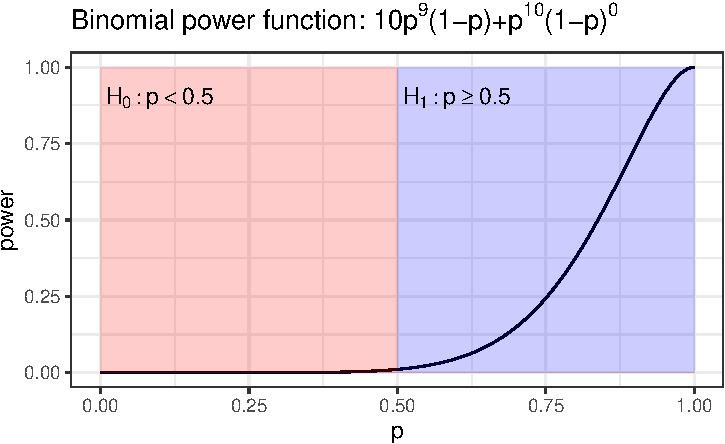
\includegraphics[width=1\linewidth]{class_notes_files/figure-latex/unnamed-chunk-5-1} \end{center}

At \(p=1/2\), the power of the test is 0.011. For \(p< 1/2\) the values
are all less than 0.011. For \(p>1/2\) the values increase with \(p\).

\hypertarget{size-and-level-of-tests}{%
\subsubsection{Size and level of tests}\label{size-and-level-of-tests}}

Generally we can't make both error probabilities as small as we'd like
for a fixed sample size. A common approach is to put a bound on the type
I error probability and find a good test (or `best' test if you can)
among those with P(type I error) \(\leq\) bound.

\noindent {\bf Definition 8.3.5} For \(0\leq \alpha \leq 1\), a test
with power function \(\beta(\theta)\) is a \emph{size \(\alpha\) test}
if \(\sup_{\theta \in \Theta_0} \beta(\theta) = \alpha\).
\noindent {\bf Definition 8.3.6} For \(0\leq \alpha \leq 1\), a test
with power function \(\beta(\theta)\) is a \emph{level \(\alpha\) test}
if \(\sup_{\theta \in \Theta_0} \beta(\theta) \leq \alpha\).

Different authors may use different definitions for size and level. In
C\&B, all size \(\alpha\) tests are also level \(\alpha\) tests. (For
level \(\alpha\) tests, the maximum type I error may be strictly less
than \(\alpha\))

In planning a study (such as a clinical trial), researchers will often
select a sample size, so that the test for the primary hypothesis has
desired power for a specific value of \(\theta \in \Theta_0^c\) and a
specific size or level.

In the previous section we found the form of the rejection region of a
variety of tests without specifying the details for the RR. That is, the
test may have been of the form \(\bXbar \geq c\) without specification
of the value \(c\). Using a condition for the size of the test, let us
identify the value of \(c\).

\noindent {\bf Example (Example 8.3.3 Normal power function)} Let
\(X_1, \ldots, X_n \sim_{iid} Normal(\mu, \sigma^2), \sigma^2\) known.
We choose our hypotheses:
\[H_0: \mu \leq \mu_0 \mbox{ versus } H_1: \mu > \mu_0\]

Let's use Theorem 8.2.4 which says we can use the distribution of our
sufficient statistic \(T(X) = \bXbar ~ \Nsc(\mu, \frac{\sigma^2}{n})\).
So, the likelihood is
\[\Lsc(\mu | \xbar) = (2\pi\sigma^2/n)^{-1} \exp\left(\frac{-(\xbar-\mu)^2}{2\sigma^2/n}\right)\]

If we maximize this likelihood in the full parameter space, we get the
MLE \(\muhat = \bxbar\).

If \(\mu_0 < \xbar\) we have \(\muhat_0 = \mu_0\). So the LRT in this
case is

\[\lambda(\xbar) = \frac{(2\pi\sigma^2/n)^{-1} \exp\left(\frac{-(\xbar-\mu_0)^2}{2\sigma^2/n}\right)}{(2\pi\sigma^2/n)^{-1} \exp\left(\frac{-(\xbar-\xbar)^2}{2\sigma^2/n}\right)} = 
\exp\left(\frac{-(\xbar-\mu_0)^2}{2\sigma^2/n}\right)\].

If \(\mu_0 \geq \xbar\) we have \(\muhat_0 = \xbar\) and so the LRT = 1.

Hence, the LRT is

\[\lambda(\xbar) = \begin{cases}
1, & \mu_0 \geq \xbar\\
\exp\left(\frac{-(\xbar-\mu_0)^2}{2\sigma^2/n}\right), & mu_0 < \bxbar
\end{cases}
\]

and the rejection region is

\begin{align*}
\Rsc &= \left\{\bx : \exp\left(\frac{-(\xbar-\mu_0)^2}{2\sigma^2/n}\right) \leq c\right\}\\
&=\left\{\bx : |\xbar-\mu_0| \geq \sqrt{-2\sigma^2\log(c)/n}\right\}\\
&= \left\{\bx : \xbar \geq \mu_0 + \sqrt{-2\sigma^2\log(c)/n}\right\}\\
&= \left\{\bx: \xbar \geq k\right\}
\end{align*}

The LRT rejects \emph{iff} \(\xbar \geq k\). To obtain a size \(\alpha\)
test, choose \(k\), so that
\(\sup_{\mu \leq \mu_0} P(\bXbar \geq k) = \alpha\). Then the power
function is:

\begin{align*}
 \beta(\mu) = P_\mu(\bXbar\geq k) &= P_\mu \left(\frac{\bXbar - \mu}{\sigma/\sqrt{n}} \geq \frac{k - \mu}{\sigma/\sqrt{n}}\right)\\
&=P_\mu \left(Z \geq \frac{k - \mu}{\sigma/\sqrt{n}}\right)\\
&= 1 - \Phi\left(\frac{k - \mu}{\sigma/\sqrt{n}} \right)
\end{align*} where \(Z\) is a standard normal variable and \(\Phi(z)\)
is the cdf of a Normal(0,1) variable. This is an increasing function of
\(\mu\) for any fixed \(k, n,\) and \(\sigma\). So the supremum of this
function with respect to \(\mu\) under \(H_0\) occurs at
\(\mu = \mu_0\). So, to determine the size we have:
\[\alpha =  \sup_{\mu \leq \mu_0}\beta(\mu) = \beta(\mu_0) = 1 - \Phi\left(\frac{k - \mu_0}{\sigma/\sqrt{n}} \right)\]
Now if we use the standard normal distribution to calculate \(z_\alpha\)
such that \(1-\Phi(z_\alpha) = P(Z > z_\alpha) = \alpha\) we have:
\[k = \mu_0 + z_\alpha\frac{\sigma}{\sqrt{n}}.\]

For example, if \(\alpha = 0.05\), we have \(z_\alpha = 1.64\)
(approximately) as \(1-\Phi(1.64) = 1 - P(Z\leq 1.64) \approx 0.05\).

Now we have found an appropriate \(k\) to keep the size at \(\alpha\).
So, our LRT rejection region is:
\[\Rsc = \left\{\bx: \bxbar \geq \mu_0 + z_\alpha\sigma/\sqrt{n}\right\}\]
and our power function is:

\begin{align*}
\beta(\mu) &= P_\mu\left(\bXbar\geq \mu_0 + z_\alpha\frac{\sigma}{\sqrt{n}}\right) = 1 - \Phi\left(\frac{\mu_0 - \mu}{\sigma/\sqrt{n}} + z_\alpha\right)
\end{align*}

We can plot \(\beta(\mu)\) for various \(\mu_0\):

\begin{Shaded}
\begin{Highlighting}[]
\NormalTok{ss <-}\StringTok{ }\DecValTok{3} \CommentTok{# sigma}
\NormalTok{nn <-}\StringTok{ }\DecValTok{20}
\NormalTok{alpha <-}\StringTok{ }\FloatTok{0.05}
\NormalTok{mydata <-}\StringTok{ }\KeywordTok{crossing}\NormalTok{(}\DataTypeTok{mu0 =} \KeywordTok{c}\NormalTok{(}\DecValTok{3}\NormalTok{,}\DecValTok{5}\NormalTok{,}\DecValTok{7}\NormalTok{), }\DataTypeTok{mu =} \KeywordTok{seq}\NormalTok{(}\DecValTok{2}\NormalTok{,}\DecValTok{11}\NormalTok{,}\DataTypeTok{by=}\FloatTok{0.01}\NormalTok{)) }\OperatorTok
\StringTok{  }\KeywordTok{mutate}\NormalTok{(}\DataTypeTok{power =} \DecValTok{1}\OperatorTok{-}\KeywordTok{pnorm}\NormalTok{((mu0}\OperatorTok{-}\NormalTok{mu)}\OperatorTok{/}\NormalTok{(ss}\OperatorTok{/}\KeywordTok{sqrt}\NormalTok{(nn))}\OperatorTok{+}\KeywordTok{qnorm}\NormalTok{(}\DecValTok{1}\OperatorTok{-}\NormalTok{alpha)),}
         \DataTypeTok{mu0 =} \KeywordTok{factor}\NormalTok{(mu0))}
\KeywordTok{ggplot}\NormalTok{(mydata,}\KeywordTok{aes}\NormalTok{(}\DataTypeTok{x =}\NormalTok{ mu, }\DataTypeTok{y =}\NormalTok{ power, }\DataTypeTok{color=}\NormalTok{mu0))}\OperatorTok{+}
\StringTok{  }\KeywordTok{geom_line}\NormalTok{()}\OperatorTok{+}
\StringTok{  }\KeywordTok{ggtitle}\NormalTok{(}\KeywordTok{TeX}\NormalTok{(}\StringTok{"Normal power curve $}\CharTok{\textbackslash{}\textbackslash{}}\StringTok{beta(}\CharTok{\textbackslash{}\textbackslash{}}\StringTok{mu)$; n = 20, $}\CharTok{\textbackslash{}\textbackslash{}}\StringTok{sigma$ = 3, $}\CharTok{\textbackslash{}\textbackslash{}}\StringTok{alpha$ = 0.05"}\NormalTok{))}\OperatorTok{+}
\StringTok{  }\KeywordTok{geom_hline}\NormalTok{(}\KeywordTok{aes}\NormalTok{(}\DataTypeTok{yintercept=}\DecValTok{1}\OperatorTok{-}\KeywordTok{pnorm}\NormalTok{(}\KeywordTok{qnorm}\NormalTok{(}\DecValTok{1}\OperatorTok{-}\NormalTok{alpha)}\OperatorTok{-}\KeywordTok{sqrt}\NormalTok{(nn)}\OperatorTok{/}\DecValTok{2}\NormalTok{)),}\DataTypeTok{color=}\StringTok{"black"}\NormalTok{,}\DataTypeTok{lty=}\DecValTok{2}\NormalTok{)}\OperatorTok{+}
\StringTok{  }\KeywordTok{annotate}\NormalTok{(}\StringTok{"text"}\NormalTok{,}\DataTypeTok{x=}\DecValTok{3}\NormalTok{,}\DataTypeTok{y=}\NormalTok{.}\DecValTok{77}\NormalTok{,}\DataTypeTok{label=}\KeywordTok{TeX}\NormalTok{(}\StringTok{"$}\CharTok{\textbackslash{}\textbackslash{}}\StringTok{beta(}\CharTok{\textbackslash{}\textbackslash{}}\StringTok{mu_0+}\CharTok{\textbackslash{}\textbackslash{}}\StringTok{sigma/2)$"}\NormalTok{))}\OperatorTok{+}
\StringTok{  }\KeywordTok{scale_color_discrete}\NormalTok{(}\DataTypeTok{name=}\KeywordTok{TeX}\NormalTok{(}\StringTok{"$}\CharTok{\textbackslash{}\textbackslash{}}\StringTok{mu_0$"}\NormalTok{))}
\end{Highlighting}
\end{Shaded}

\begin{center}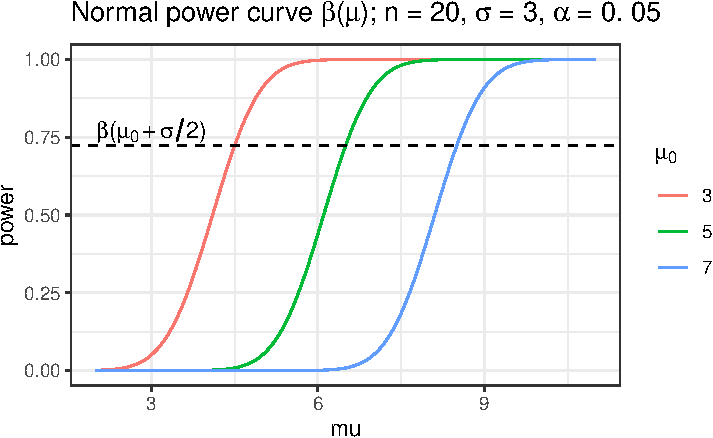
\includegraphics[width=1\linewidth]{class_notes_files/figure-latex/plot_normal_power_curve-1} \end{center}

How do we determine power under the alternative? When the size and
\(\mu_0\) is fixed, power depends on \(\mu\) and \(n\). Suppose we care
about a specific \(\mu_1\) in the alternative space,
\(\mu_1 = \mu_0 + \sigma/2\). Now we can calculate the power of our test
under the alternative at this particular \(\mu_1\):

\begin{align*}
\beta(\mu_0 + \sigma/2) &= 1 - \Phi\left(\frac{\mu_0 - (\mu_0 + \sigma/2)) }{\sigma/\sqrt{n}} + z_\alpha\right)\\
&= 1- \Phi\left(z_\alpha - \sqrt{n}/2\right)
\end{align*}

We see that this is now a function of \(n\). So, for example, if we set
our size to be \(\alpha = 0.05\) then we have \(z_\alpha = 1.64\), and
if we have \(n=20\), then the power at \(\mu_1 = \mu_0 + \sigma/2\) is
\(1-\Phi(1.64-\sqrt{20}/2) \approx 0.72\) which we can see in the plot
above at \(\mu_1 = \mu_0+3/2\) for each \(\mu_0\).

We can also plot power for a fixed \(\mu_0\) and various \(n\):

\begin{Shaded}
\begin{Highlighting}[]
\NormalTok{ss <-}\StringTok{ }\DecValTok{3} \CommentTok{# sigma}
\NormalTok{alpha <-}\StringTok{ }\FloatTok{0.05}
\NormalTok{mydata <-}\StringTok{ }\KeywordTok{crossing}\NormalTok{(}\DataTypeTok{nn =} \KeywordTok{c}\NormalTok{(}\DecValTok{5}\NormalTok{,}\DecValTok{20}\NormalTok{,}\DecValTok{100}\NormalTok{), }\DataTypeTok{mu0 =} \DecValTok{5}\NormalTok{, }\DataTypeTok{mu =} \KeywordTok{seq}\NormalTok{(}\DecValTok{2}\NormalTok{,}\DecValTok{11}\NormalTok{,}\DataTypeTok{by=}\FloatTok{0.01}\NormalTok{)) }\OperatorTok
\StringTok{  }\KeywordTok{mutate}\NormalTok{(}\DataTypeTok{power =} \DecValTok{1}\OperatorTok{-}\KeywordTok{pnorm}\NormalTok{((mu0}\OperatorTok{-}\NormalTok{mu)}\OperatorTok{/}\NormalTok{(ss}\OperatorTok{/}\KeywordTok{sqrt}\NormalTok{(nn))}\OperatorTok{+}\KeywordTok{qnorm}\NormalTok{(}\DecValTok{1}\OperatorTok{-}\NormalTok{alpha)),}
         \DataTypeTok{nn_fac =} \KeywordTok{factor}\NormalTok{(nn))}
\KeywordTok{ggplot}\NormalTok{(mydata,}\KeywordTok{aes}\NormalTok{(}\DataTypeTok{x =}\NormalTok{ mu, }\DataTypeTok{y =}\NormalTok{ power, }\DataTypeTok{color=}\NormalTok{nn_fac))}\OperatorTok{+}
\StringTok{  }\KeywordTok{geom_line}\NormalTok{()}\OperatorTok{+}
\StringTok{  }\KeywordTok{ggtitle}\NormalTok{(}
    \KeywordTok{TeX}\NormalTok{(}\StringTok{"Normal power curve $}\CharTok{\textbackslash{}\textbackslash{}}\StringTok{beta(}\CharTok{\textbackslash{}\textbackslash{}}\StringTok{mu)$; $}\CharTok{\textbackslash{}\textbackslash{}}\StringTok{mu_0$ = 5, $}\CharTok{\textbackslash{}\textbackslash{}}\StringTok{sigma$ = 3, $}\CharTok{\textbackslash{}\textbackslash{}}\StringTok{alpha$ = 0.05"}\NormalTok{))}\OperatorTok{+}
\StringTok{  }\KeywordTok{geom_hline}\NormalTok{(}\KeywordTok{aes}\NormalTok{(}\DataTypeTok{yintercept=}\DecValTok{1}\OperatorTok{-}\KeywordTok{pnorm}\NormalTok{(}\KeywordTok{qnorm}\NormalTok{(}\DecValTok{1}\OperatorTok{-}\NormalTok{alpha)}\OperatorTok{-}\KeywordTok{sqrt}\NormalTok{(nn)}\OperatorTok{/}\DecValTok{2}\NormalTok{), }\DataTypeTok{color=}\NormalTok{nn_fac),}\DataTypeTok{lty=}\DecValTok{2}\NormalTok{)}\OperatorTok{+}
\StringTok{  }\KeywordTok{geom_vline}\NormalTok{(}\DataTypeTok{xintercept =} \DecValTok{5}\NormalTok{, }\DataTypeTok{lty=}\DecValTok{3}\NormalTok{)}\OperatorTok{+}
\StringTok{  }\KeywordTok{annotate}\NormalTok{(}\StringTok{"text"}\NormalTok{,}\DataTypeTok{x=}\DecValTok{3}\NormalTok{,}\DataTypeTok{y=}\NormalTok{.}\DecValTok{77}\NormalTok{,}\DataTypeTok{label=}\KeywordTok{TeX}\NormalTok{(}\StringTok{"$}\CharTok{\textbackslash{}\textbackslash{}}\StringTok{beta(}\CharTok{\textbackslash{}\textbackslash{}}\StringTok{mu_0+}\CharTok{\textbackslash{}\textbackslash{}}\StringTok{sigma/2)$"}\NormalTok{))}\OperatorTok{+}
\StringTok{  }\KeywordTok{scale_color_discrete}\NormalTok{(}\DataTypeTok{name=}\StringTok{"n (sample size)"}\NormalTok{)}
\end{Highlighting}
\end{Shaded}

\begin{center}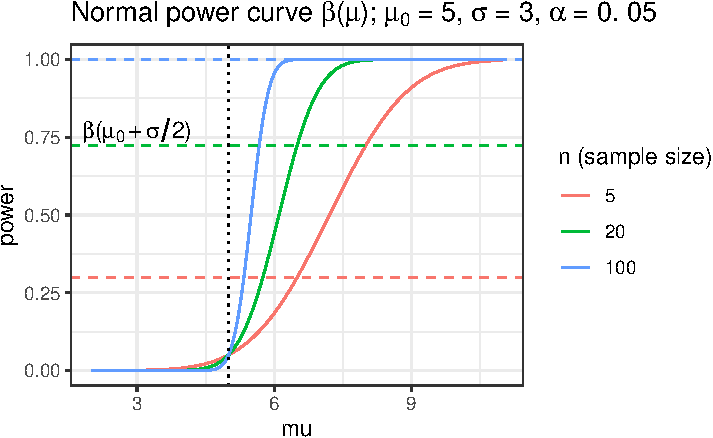
\includegraphics[width=1\linewidth]{class_notes_files/figure-latex/plot_normal_power_curve_n-1} \end{center}

Now we see that \(\beta(\mu_0 + \sigma/2)\) increases with \(n\).

\hypertarget{unbiased-tests}{%
\subsubsection{Unbiased tests}\label{unbiased-tests}}

We would like a test we use to have at least as good power when the
alternative is true as when the null hypothesis is true. In other words
we want our power \emph{under the alternative} to be higher than the
\emph{level} of our test (type I error). Tests that satisfy this
property are referred to as unbiased.

\noindent {\bf Definition 8.3.9} A test with power function
\(\beta(\theta)\) is \emph{unbiased} if
\(\beta(\theta^\prime) \geq \beta(\theta^{\prime\prime})\) for every
\(\theta^\prime \in \Theta_0^C\) and
\(\theta^{\prime\prime} \in \Theta_0\).

\noindent {\bf Example (Example 8.3.10 Conclusion of 8.3.3 Normal power function)}
We saw earlier that the power function for the size \(\alpha\) LRT of
\(H_0: \mu \leq \mu_0\) versus \(H_1: \mu > \mu_0\) was monotone
increasing in \(\mu\), so the power for any \(\mu\) such that
\(\mu > \mu_0\) is greater than the power for any such \(\mu\) such that
\(\mu \leq \mu_0\). Hence the LRT test for this setting is unbiased. We
see this in the plot of the power function above where the power
function is always larger than \(\alpha = 0.05\) when \(\mu > \mu_0\).

\hypertarget{most-powerful-tests}{%
\subsubsection{Most powerful tests}\label{most-powerful-tests}}

There can be many size \(\alpha\) tests for a given problem, also many
unbiased tests for a given problem, so we will look for additional
criteria to select a good test. The first consideration will be to find
the most powerful level \(\alpha\) test.

\noindent {\bf Definition 8.3.11} Let \(\Cbb\) be a class of tests for
testing \(H_0: \theta \in \Theta_0\) versus
\(H_1: \theta \in \Theta_0^C\). A test in class \(\Cbb\), with power
function \(\beta(\theta)\), is a \textbf{uniformly most powerful (UMP)}
class \(\Cbb\) test if \(\beta(\theta)\geq \beta^\prime(\theta)\) for
every \(\theta \in \Theta_0^C\) and every \(\beta^\prime(\theta)\) that
is a power function of a test in class \(\Cbb\).

First we will consider the class \(\Cbb\) to be the class of all level
\(\alpha\) tests. We find the UMP level \(\alpha\) test (when it exists)
using the following theorem.

\noindent {\bf Theorem 8.3.12: Neyman-Pearson Lemma} Consider testing
\(H_0: \theta = \theta_0\) versus \(H_1 : \theta = \theta_1\), where the
pdf or pmf corresponding to \(\theta_i\) is
\(f(\bx | \theta_i), i = 0,1\) using a test with \emph{rejection region}
\(\Rsc\) that satisfies (8.3.1):
\[\bx \in \Rsc \mbox{ if } f(\bx|\theta_1) > k f(\bx | \theta_0), \mbox{ and }\]
\[\bx \in \Rsc^c \mbox{ if } f(\bx|\theta_1) < k f(\bx | \theta_0),\]
for some \(k\geq 0\), and (8.3.2):
\[ \alpha = P_{\theta_0} (\bX \in \Rsc).\] Then:

\begin{enumerate}
\def\labelenumi{\alph{enumi})}
\tightlist
\item
  (\emph{Sufficiency}) Any test that satisfies the above conditions
  (8.3.1 and 8.3.2) is a UMP level \(\alpha\) test.
\item
  (\emph{Necessity}) If there exists a test satisfying the above
  conditions (8.3.1 and 8.3.2) with \(k>0\), then every UMP level
  \(\alpha\) test is a size \(\alpha\) test and every UMP level
  \(\alpha\) test satisfies 8.3.1 (except perhaps on a set that has
  probability zero when \(\theta = \theta_0\) and
  \(\theta = \theta_1\)).
\end{enumerate}

\noindent {\bf Proof}: See C\&B. Note that
\(\alpha = P_{\theta_0} (\bX \in \Rsc)\) implies a size \(\alpha\) test
and hence a level \(\alpha\) test since \(\Theta_0\) has only one point.

\noindent {\bf Note} we are not saying anything about the form of the
test when \(f(\bx|\theta_1) = k f(\bx| \theta_0)\).

\noindent {\bf Note}, also, we can write the rejection region as
\[\Rsc = \left\{ \bx: \frac{f(\bx | \theta_1)}{f(\bx | \theta_0)} > k\right\}\]
and
\[\Rsc^c = \left\{ \bx: \frac{f(\bx | \theta_1)}{f(\bx | \theta_0)} < k\right\}\]
provided we are not dividing by zero. This is an easier form of the
lemma to work with.

\noindent {\bf Note} in the Neyman-Pearson Lemma there is no requirement
that the observations are \(iid\). The pdf (pmf) could be from
non-\(iid\) observations such as in a regression setting. We will see
examples of this later.

As with the LRT test, we can also first reduce by sufficiency and then
apply NP using the pdf (pmf) of the sufficient statistic.

\noindent {\bf Corollary 8.3.13: } Consider the same hypothesis problem
as in the Neyman-Pearson lemma. Suppose \(T = T(\bX)\) is sufficient for
\(\theta\) and \(g(t|\theta_i)\) is the pdf or pmf of \(T\)
corresponding to \(\theta_i, i = 0,1\). Then, any test based on \(T\)
with rejection region \(S\) is a UMP level \(\alpha\) test if it
satisfies
\[t \in S \mbox{ if } g(t|\theta_1) > k g(t | \theta_0), \mbox{ and }\]
\[t \in S^c \mbox{ if } g(t|\theta_1) < k g(t | \theta_0),\] for some
\(k\geq 0\), \[\alpha = P_{\theta_0}(T\in S). \mbox{ (8.3.5) }\]

\noindent {\bf Proof}: By the factorization theorem, see C\&B.

It can be easier to work with the pdf (or pmf) of a sufficient reduction
of the data and hence this theorem is useful.

We can write the rejection region as

\[\Ssc = \left\{ \bx: \frac{g(\bt | \theta_1)}{g(\bt | \theta_0)} > k\right\}\]

\noindent{\bf Example (Example 8.3.14 UMP binomial test}: Let
\(X \sim Binomial(2,\theta)\). We want to test
\[H_0:  \theta = 1/2 \mbox{ versus } H_1: \theta = 3/4.\]

We can use Neyman-Pearson lemma by calculating
\[\frac{f(\bx | \theta_1)}{f(\bx | \theta_0)} \] for each possible value
of \(\bx\), and finding a constant \(k\) that satisfies the lemma.

Calculating the ratios of the pmfs gives:
\[\frac{f(0|\theta = 3/4)}{f(0|\theta = 1/2)} = \frac{1}{4},
\frac{f(1|\theta = 3/4)}{f(1|\theta = 1/2)} = \frac{3}{4}, \mbox{ and } \frac{f(2|\theta = 3/4)}{f(2|\theta = 1/2)} = \frac{9}{4}\]

We need to choose a rejection region and \(k\).

If we choose \(3/4 < k < 9/4\), the NP lemma says that the rejection
region \(\Rsc = \{X = 2\}\) is the UMP test with level
\(\alpha = \sup_{\theta = 1/2} \beta(\theta)= P(X=2 | \theta = 1/2) = 1/4\).
This is because for
\[\bx \in \Rsc , \, \frac{f(\bx | \theta_1)}{f(\bx | \theta_0)} > k\]
and for
\[ \bx \in \Rsc^c , \, \frac{f(\bx | \theta_1)}{f(\bx | \theta_0)} < k.\]

On the other hand, if the rejection region is
\(\{X =1 \mbox{ or } 2\}\), the NP lemma is satisfied with
\(1/4 < k < 3/4\) and so this test is UMP level
\(\alpha = P(X = 1 \mbox{ or } 2 | \theta = 1/2) = 3/4\) test.

For extreme (trivial) cases, a \(k < 1/4\) would correspond to the UMP
test with rejection region \(\{ X >= 0\}\) and level
\(\alpha = P(X >= 0 | \theta = 1/2) = 1\), and if \(k > 9/4\) yields the
UMP test with rejection region \(X > 2\}\) and level
\(\alpha = P(X > 2 | \theta = 1/2) = 0\).

\textbf{Note:} this shows that for a discrete distribution, the
\(\alpha\) level at which a test can be done is a function of the
particular pmf of the data. No such problem arises in the continuous
case. Any \(\alpha\) level can be attained.

\noindent {\bf Example (Example 8.3.15 UMP normal test)}: Again we have
\(X_i \sim_{iid} N(\mu,\sigma^2)\) with \(\sigma^2\) known. The same
mean \(\bXbar\) is the sufficient statistic for \(\mu\). Consider
testing \(H_0: \mu = \mu_0\) versus \(H_1: \mu = \mu_1\) where
\(\mu_0 > \mu_1\). The inequality
\[g(\bxbar | \mu_1) > k g(\bxbar | \mu_0)\] is equivalent to
\begin{align*}
\frac{\sqrt{n}}{\sigma\sqrt{2\pi}}e^{-n(\bxbar - \mu_1)^2/(2\sigma^2)} &> k \frac{\sqrt{n}}{\sigma\sqrt{2\pi}}e^{-n(\bxbar - \mu_0)^2/(2\sigma^2)} \Longleftrightarrow\\
(\bxbar - \mu_1)^2 & <(2\sigma^2 \log(k))/n + (\bxbar - \mu_0)^2\\
\bxbar &< \frac{(2\sigma^2 \log(k))/n - \mu_0^2 + \mu_1^2}{2(\mu_0 - \mu_1)}.
\end{align*}

The right-hand side increases from \(-\infty\) to \(\infty\) as \(k\)
increases from \(0\) to \(\infty\). Thus, by Corollary 8.3.13, the test
with rejection region \(\bxbar < c\) is the UMP level \(\alpha\) test,
where \(\alpha = P_{\mu_0}(\bXbar < c)\). If a particular \(\alpha\) is
specified, then the UMP test rejects \(H_0\) if
\(\bXbar < c = \mu_0 -\sigma z_\alpha /\sqrt{n}\) (from above size
calculations). This choice of \(c\) ensures that 8.3.5 is true.

\newpage

\hypertarget{composite-hypotheses}{%
\subsubsection{Composite hypotheses}\label{composite-hypotheses}}

The NP lemma and corollary are concerned with \emph{simple} hypotheses
where only one distribution is specified by \(H_0\) and \(H_1\). In most
realistic problems, the hypotheses of interest specify more than one
possible distribution for the sample and are \emph{composite}
hypotheses.

For instance, suppose we are interested in a test of the form
\(H_0: \mu \leq \mu_0\) versus \(H_1: \mu > \mu_0\), where, here we can
see that each of the two hypotheses contain several parameter values
(and hence several distributions). These types of hypotheses are
composite hypotheses and in fact is a \emph{one-sided} hypothesis.

The Neyman Pearson Lemma in many cases can be extended to composite
hypotheses. In particular this may be the case for certain one-sided
hypotheses.

For two-sided hypotheses, such as \(H: \theta \neq \theta_0\), we cannot
typically extend NP to get UMP tests.

For tests of one-sided hypotheses some distributions have a property
that readily leads to UMP tests.

\noindent {\bf Definition 8.3.16} A family of pdfs or pmfs
\(\{ f(x|\theta): \theta \in \Theta\}\) for a univariate random variable
\(X\) with real valued parameter \(\theta\) has a
\textbf{monotone likelihood ratio (MLR)} if for every
\(\theta_1 > \theta_2\)
\[ \frac{f(t|\theta_1)}{f(t|\theta_2)} = V(T(X), \theta_1, \theta_2)\]
where \(V(T, \theta_1, \theta_2)\) is a monotone \emph{non-decreasing}
function of \(T\).

\textbf{Notes}

\begin{itemize}
\tightlist
\item
  \(c/0\) is defined as \(\infty\) if \(c>0\)
\item
  C\&B define MLR slightly differently, using the distribution of
  \(T(X)\). This is equivalent due to the factorization and
  transformation theorems! C\&B also define MLR as \emph{either}
  monotone non-decreasing or non-increasing, but we need non-decreasing
  for the big theorem in this section.
\item
  Many common families of distributions have an MLR. \emph{Any regular
  exponential family with
  \(f(x|\theta) = h(x) c(\theta) e^{w(\theta) T(x)}\) has an MLR if
  \(w(\theta)\) is a non-decreasing function.} For example, normal
  (known variance, unknown mean), Poisson, and binomial all have an MLR.
\end{itemize}

\textbf{Example: Bernoulli distribution} Consider a family of Bernoulli
distributions \(\{B(p): p \in [0,1]\}\). The ratio of joint pmf of
\(X_1, \ldots, X_n\) is

\[\frac{f(\bX| p_1)}{f(\bX | p_2)} = \frac{p_1^{\sum X_i} (1-p_1)^{n-\sum X_i}}{p_2^{\sum X_i}(1-p_2)^{n-\sum X_i}} = 
\left( \frac{1-p_1}{1-p_2}\right)^n \left( \frac{p_1(1-p_2)}{p_2(1-p_1)}\right)^{\sum X_i} \]

For \(p_1 > p_2\), \[\frac{p_1(1-p_2)}{p_2(1-p_1)} > 1\]

and, therefore, the likelihood ratio is monotone increasing
(non-decreasing) in \(T(\bX) = \sumin X_i\).

Other ways to prove MLR: We could have also written this ratio as a
function of \(T\):

\[V(t) = \left( \frac{1-p_1}{1-p_2}\right)^n \left( \frac{p_1(1-p_2)}{p_2(1-p_1)}\right)^{t} \]
with derivative
\[\frac{\partial}{\partial t}V(t) =  \left( \frac{1-p_1}{1-p_2}\right)^n t \left( \frac{p_1(1-p_2)}{p_2(1-p_1)}\right)^{t-1} \]
which is a product of three numbers \(\geq0\), so the derivative is
\(\geq 0\), and hence the ratio \(V(t)\) is non-decreasing in \(t\).

We could have also written the joint distribution as a regular
exponential family where \(w(p) = \log(p/(1-p))\), a non-decreasing
function of \(p\), since
\[f(\bx|p) = p^{\sum_i x_i} (1-p)^{n-\sum_i x_i} = (1-p) \left( \frac{p}{1-p}\right)^{\sum_i x_i} = (1-p)^n \exp\left[ \left(\log \frac{p}{1-p}\right)\sum_i x_i\right].\]

\textbf{Example: Exponential distribution} Consider a family of
Exponential distributions \(\{Exp(\beta): \beta \in (0,\infty)\}\). The
ratio of joint pmf of \(X_1, \ldots, X_n\) is
\[\frac{f(\bX| \beta_1)}{f(\bX | \beta_2)} = \frac{\beta_1^{-1}\exp(-\sum X_i/\beta_1)}{\beta_2^{-1}\exp(-\sum X_i/\beta_2)} =
\left(\frac{\beta_2}{\beta_1}\right)\exp(\sum X_i / \beta_2 - \sum X_i/\beta_1) = 
\left(\frac{\beta_2}{\beta_1}\right) \exp \left[\frac{\beta_1 - \beta_2}{\beta_1\beta_2}\sum X_i \right]
\] Since \(\frac{\beta_1 - \beta_2}{\beta_1\beta_2} > 0\), this ratio is
monotone non-decreasing in \(T(\bX) = \sum X_i\).

Other ways to prove MLR: We could also have written this as a regular
exponential family where \(w(\beta) = -1/\beta\) which is a
non-decreasing function of \(\beta\). We could have also taken the
derivative of the ratio with respect to \(t\) and shown it is
\(\geq 0\).

\textbf{Theorem 8.3.17 (Karlin-Rubin)} Consider testing
\[H_0: \theta \leq \theta_0 \mbox{ versus } H_1: \theta > \theta_0.\]
Suppose, for any \(t_0\),

\begin{enumerate}
\item $T$ is a sufficient statistic for $\theta$ and
\item the family of pdfs or pmfs $\{f(x|\theta): \theta \in \Theta\}$ of an MLR in $T$
\item $\alpha = P_{\theta_0} (T >t_0$)
\end{enumerate}

\noindent Then the test with rejection region \[\Rsc = \{t: T> t_0\}\]
is a \textbf{UMP level \(\alpha\) test}.

Conversely, if testing
\[H_0: \theta \geq \theta_0 \mbox{ versus } H_1: \theta < \theta_0,\]
with \(T\) a sufficient statistic for \(\theta\) and
\(\{f(x|\theta): \theta \in \Theta\}\) has an MLR in \(T\). Then for any
\(t_0\), the \(\Rsc = \{t: T< t_0\}\) is a UMP level \(\alpha\) test,
where \(\alpha = P_{\theta_0} (T < t_0)\).

\noindent {\bf Proof:} In book. Essentially, the MLR allows us to use
Neyman Pearson Lemma for any \(\theta_1\) in \(\Theta_0\) and
\(\theta_2\) in \(\Theta_1\). We have the correct size test because the
MLR gives us a power function \(\beta(\theta) = P_\theta(T>t_0)\) that
is also non-decreasing in \(\theta\).

\textbf{Example: Exponential}

Suppose we have \(X_1, \ldots X_n \sim\) Exp(\(\beta\)). We wish to test
the hypothesis:
\[H_0: \beta \leq \beta_0 \mbox{ versus } H_1: \beta > \beta_0.\]

Can we find a UMP size \(\alpha\) test?

From above we know that this family of distributions has an MLR in
\(T(\bX) = \sumin X_i\). So we can reject the null hypothesis with
rejection region \[\Rsc = \left\{\bx: \sumin X_i > t_0\right\}\]

where \(t_0\) is selected to satisfy the equation
\[\alpha = P_{\beta_0}\left(\sumin X_i > t_0\right)\]

To solve for \(t_0\), we use the fact that
\(\sumin X_i \sim \Gamma_{n, \beta} = \mbox{Gamma}(n,\beta)\) and so
\(t_0 = \gamma_{\alpha, n, \beta_0}\) which is the critical value of a
Gamma(\(n, \beta_0\)) distribution such that

\[\alpha = P_{\beta_0}\left(\Gamma_{n, \beta_0} > \gamma_{\alpha, n, \beta_0}\right)\]

\noindent {\bf Example: Normal UMP Test continued (Ex 8.3.18, continuation of Ex 8.3.15)}

Again we have our normal data with variance known. Consider testing
\[H_0: \mu \geq \mu_0 \mbox{ versus } H_1: \mu < \mu_0\] using the test
with rejection region:
\[\Rsc = \{\bx: \bxbar < \mu_0 - \sigma z_\alpha/\sqrt{n}\}.\]

Let's \textbf{show this test is UMP and size } \(\alpha\).

As \(\bXbar\) is sufficient and its distribution is
Normal(\(\mu, \sigma^2/n\)) with variance known and so is a
one-dimensional exponential family with \(w(\mu) = \mu/(2\sigma^2)\)
increasing in \(\mu\), it follows from Karlin-Rubin Theorem (Thm 8.3.17)
that the test is a UMP level \(\alpha\) test in this problem.

We know the power of this test
\[\beta(\mu) = P_{\mu}(\bXbar < \mu_0 - \sigma z_\alpha/\sqrt{n}) = 
P\left(Z < \frac{\mu_0 - \mu}{\sigma/\sqrt{n}}+ z_\alpha\right) = \Phi\left(\frac{\mu_0 - \mu}{\sigma/\sqrt{n}}+ z_\alpha\right)\]
is a decreasing function of \(\mu\) since \(\mu\) is a location
parameter in the distribution of \(\bXbar\) and so \(\beta(\mu)\) is
maximized in the null hypothesis space at \(\mu_0\) and
\(\beta(\mu_0) = \alpha\).

\noindent {\bf Example: Two-sided Normal Test (Example 8.3.19)} Now
consider the same Normality setting but with a two-sided test:
\[H_0: \mu = \mu_0 \mbox{ versus } H_1: \mu\neq\mu_0.\] Can we find a
UMP level \(\alpha\) test in this setting?

Consider first the above one-sided test where we have
\(H^*_0: \mu \geq \mu_0\) versus \(H^*_1: \mu < \mu_0\) and the UMP
level \(\alpha\) test rejects this \(H^*_0\) if
\(\bXbar < \mu_0 - z_\alpha \sigma/\sqrt{n}\). Let the power of this
test be \(\beta^*(\mu)\) and call this Test 1. Recall by NP Lemma that
the best test must be of this form except on a set that has probability
zero.

Conversely, if we wish to test \(H^{**}_0: \mu \leq \mu_0\) against
\(H^{**}_1: \mu > \mu_0\) we can prove that the UMP level \(\alpha\)
test that rejects if \(\bXbar > \mu_0 + z_\alpha \sigma/\sqrt{n}\). Let
the power of this test be \(\beta^{**}(\mu)\) and call it Test 2.

Now consider \(\mu_1 > \mu_0\) which falls under the null hypothesis
space of \(H^*_0\) and the alternative space \(H^{**}_1\). Let's
evaluate the power of the second one-sided test at \(\mu_1\):
\begin{align*}
\beta^{**}(\mu_1) &= P_{\mu_1} (\bXbar > \mu_0 + z_\alpha \sigma/\sqrt{n})\\
&= P_{\mu_1} \left(\frac{\bXbar - \mu_1}{\sigma/\sqrt{n}} > \frac{\mu_0 - \mu_1}{\sigma/\sqrt{n}}+ z_\alpha\right)\\
&> P(Z > z_\alpha)\\
&= P(Z < -z_\alpha)\\
&> P_{\mu_1} \left(\frac{\bXbar - \mu_1}{\sigma/\sqrt{n}} < \frac{\mu_0 - \mu_1}{\sigma/\sqrt{n}}- z_\alpha\right)\\
&= P_{\mu_1} (\bXbar < \mu_0 - z_\alpha \sigma/\sqrt{n})\\
&= \beta^{*}(\mu_1)
\end{align*}

So, the power of the Test 2 at \(\mu_1\) is greater than the power of
Test 1 at \(\mu_1\). Hence, Test 1 cannot be the best test for all
\(\mu\). But, recall the best test had to be of that form. So, no best
test exists.

You can see in the plot below that although Test 1 and Test 2 have
slightly higher powers than Test 3 for some parameter points, Test 3 has
much higher power than Test 1 and Test 2 at other parameter points.

So, to get a ``best'' test for a setting like this we will have to
\textbf{restrict the class of tests} we are willing to consider. The
class we will consider here is the \textbf{class of unbiased tests}.

Note in this example for Test 1 the power is high when \(\mu\) is small,
but not when \(\mu\) is large. In fact the power is \(<\alpha\) when
\(\mu > \mu_0\). The opposite is true for Test 2. We'd like the power
when the alternative hypothesis is true to be large and specifically
greater than the power under the null hypothesis. Recall, we define the
class of unbiased tests as tests with power function, \(\beta(\theta)\),
satisfying
\[\beta(\theta^\prime)\geq \beta(\theta^{\prime\prime}), \mbox{ for every, } \theta^\prime \in \Theta_0^C, \theta^{\prime\prime}\in\Theta_0.\]

Then we can often find a UMP unbiased level \(\alpha\) test for one
parameter problems involving composite hypotheses and for many two-sided
problems as well.

\noindent {\bf Example: Two-sided Normal Test Unbiased (Example 8.3.20)}\\
When no UMP level \(\alpha\) test exists within the class of all tests,
we might try to find a UMP level \(\alpha\) test within the class of
unbiased tests.

The test which rejects \(H_0: \theta = \theta_0\) in favor of
\(H_1: \theta \neq \theta_0\), if and only if
\[\bXbar > \mu_0 + z_{\alpha/2} \sigma/\sqrt{n}, \mbox{ or } \bXbar < \mu_0 - z_{\alpha/2} \sigma/\sqrt{n}\]
is a UMP unbiased level \(\alpha\) test; that is, it is UMP in the class
of unbiased tests.

\begin{Shaded}
\begin{Highlighting}[]
\NormalTok{ss <-}\StringTok{ }\DecValTok{1} \CommentTok{# sigma}
\NormalTok{alpha <-}\StringTok{ }\FloatTok{0.05}
\NormalTok{nn <-}\StringTok{ }\DecValTok{10}
\NormalTok{mydata <-}\StringTok{ }\KeywordTok{tibble}\NormalTok{(}\DataTypeTok{mu =} \KeywordTok{seq}\NormalTok{(}\OperatorTok{-}\FloatTok{1.8}\NormalTok{,}\FloatTok{1.8}\NormalTok{,}\DataTypeTok{by=}\FloatTok{0.01}\NormalTok{)) }\OperatorTok
\StringTok{  }\KeywordTok{mutate}\NormalTok{(}\DataTypeTok{upper_tail =} \DecValTok{1}\OperatorTok{-}\KeywordTok{pnorm}\NormalTok{((}\OperatorTok{-}\NormalTok{mu)}\OperatorTok{/}\NormalTok{(ss}\OperatorTok{/}\KeywordTok{sqrt}\NormalTok{(nn))}\OperatorTok{+}\KeywordTok{qnorm}\NormalTok{(}\DecValTok{1}\OperatorTok{-}\NormalTok{alpha)),}
         \DataTypeTok{lower_tail =} \KeywordTok{pnorm}\NormalTok{((}\OperatorTok{-}\NormalTok{mu)}\OperatorTok{/}\NormalTok{(ss}\OperatorTok{/}\KeywordTok{sqrt}\NormalTok{(nn))}\OperatorTok{-}\KeywordTok{qnorm}\NormalTok{(}\DecValTok{1}\OperatorTok{-}\NormalTok{alpha)),}
         \DataTypeTok{two_tail =} \DecValTok{1}\OperatorTok{+}\KeywordTok{pnorm}\NormalTok{((}\OperatorTok{-}\NormalTok{mu)}\OperatorTok{/}\NormalTok{(ss}\OperatorTok{/}\KeywordTok{sqrt}\NormalTok{(nn))}\OperatorTok{-}\KeywordTok{qnorm}\NormalTok{(}\DecValTok{1}\OperatorTok{-}\NormalTok{alpha}\OperatorTok{/}\DecValTok{2}\NormalTok{)) }\OperatorTok{-}
\StringTok{           }\KeywordTok{pnorm}\NormalTok{((}\OperatorTok{-}\NormalTok{mu)}\OperatorTok{/}\NormalTok{(ss}\OperatorTok{/}\KeywordTok{sqrt}\NormalTok{(nn))}\OperatorTok{+}\KeywordTok{qnorm}\NormalTok{(}\DecValTok{1}\OperatorTok{-}\NormalTok{alpha}\OperatorTok{/}\DecValTok{2}\NormalTok{))}
\NormalTok{         ) }\OperatorTok
\StringTok{  }\KeywordTok{gather}\NormalTok{(}\DataTypeTok{key=}\StringTok{"test"}\NormalTok{,}\DataTypeTok{value=}\StringTok{"power"}\NormalTok{,}\OperatorTok{-}\NormalTok{mu)}
\KeywordTok{ggplot}\NormalTok{(mydata,}\KeywordTok{aes}\NormalTok{(}\DataTypeTok{x =}\NormalTok{ mu, }\DataTypeTok{y =}\NormalTok{ power, }\DataTypeTok{color=}\NormalTok{test, }\DataTypeTok{lty =}\NormalTok{ test))}\OperatorTok{+}
\StringTok{  }\KeywordTok{geom_line}\NormalTok{()}\OperatorTok{+}
\StringTok{  }\KeywordTok{xlab}\NormalTok{(}\StringTok{"mu - mu0"}\NormalTok{)}\OperatorTok{+}
\StringTok{  }\KeywordTok{ylab}\NormalTok{(}\StringTok{"power function"}\NormalTok{)}\OperatorTok{+}
\StringTok{  }\KeywordTok{ggtitle}\NormalTok{(}\StringTok{"Power of upper, lower, and two-tailed test"}\NormalTok{)}
\end{Highlighting}
\end{Shaded}

\begin{center}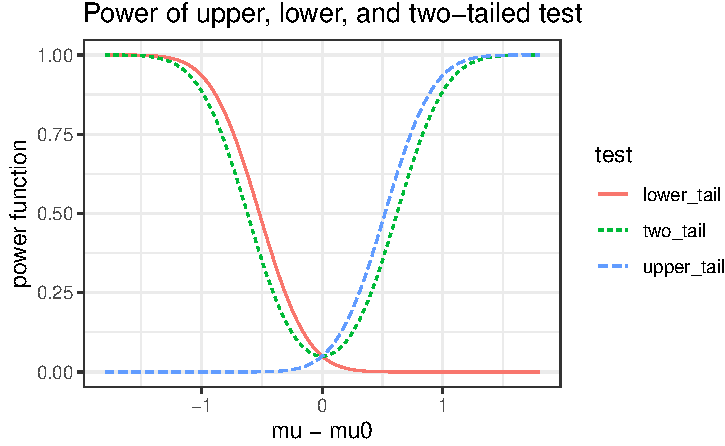
\includegraphics[width=1\linewidth]{class_notes_files/figure-latex/plot_normal_power_curve_ump-1} \end{center}

\hypertarget{p-values}{%
\subsubsection{p-values}\label{p-values}}

As you know, it is more useful to report p-values than just what the
size of the test is and what the test decision is (reject or not).

\noindent\textbf{Definition 8.3.26} A \emph{p-value} \(p(\bX\)) is a
\textbf{test statistic} satisfying \(0\leq p(\bx)\leq1\) for every
sample point \(\bx\). Small values of \(p(\bX)\) give evidence that
\(H_1\) is true.

A p-value is \emph{valid} if, for every \(\theta \in \Theta_0\) and
every \(0\leq \alpha \leq 1\),
\[P_\theta (p(\bX) \leq \alpha) \leq \alpha.\]

\begin{itemize}
\item if $p(\bX)$ is valid $\rightarrow$ can construct a level $\alpha$ test based on $p(\bX)$: the test that rejects $H_0$ if and only if $p(\bX) \leq \alpha$ is a level $\alpha$ test
\item reporting a test result via a p-value allows reader to choose the $\alpha$ he/she considers appropriate and compare reported $p(\bx)$ to $\alpha$
\item smaller p-value $\rightarrow$ stronger evidence for rejecting $H_0$
\item p-value reports the results of a test on a more continuous scale, rather than just dichotomous decision "Accept $H_0$" or "Reject $H_0$."
\end{itemize}

\noindent \textbf{Theorem 8.3.27} Let \(W(\bX)\) be a test statistic
such that large values of \(W\) give evidence that \(H_1\) is true. For
each sample point \(\bx\), define \begin{equation}
p(\bx) = \sup_{\theta\in\Theta_0} P_\theta (W(\bX) \geq W(\bx)). \tag{8.3.9}
\end{equation} Then, \(p(\bX)\) is a valid p-value.

\noindent \textbf{Proof} Fix \(\theta \in \Theta_0\). Let
\(F_\theta(w)\) denote the cdf of \(-W(\bX)\). Define
\[p_\theta(\bx) = P_\theta (W(\bX) \geq W(\bx)) = P_\theta(-W(\bX) \leq -W(\bx)) = F_\theta (-W(\bx)).\]

\begin{itemize}
\item Hence, $p_\theta (\bX)$ is a random variable and is equal to $F_\theta(-W(\bX))$.
\item By the Probability Integral Transformation, $p_\theta(\bX) \sim $Uniform(0,1) (or is stochastically equal to or greater than)
\item Hence, $P_\theta(p_\theta(\bX) \leq \alpha) \leq \alpha$ for every $0\leq \alpha \leq 1$.
\end{itemize}

Now, since
\(p(\bx) = \sup_{\theta^\prime \in \Theta_0} p_{\theta^\prime}(\bx) \geq p_\theta(\bx)\)
for every \(\bx\):
\[P_\theta(p(\bX) \leq \alpha) \leq P_\theta(p_\theta(\bX) \leq \alpha) \leq \alpha.\]
This is true for every \(\theta \in \Theta_0\) and for every
\(0\leq \alpha \leq 1 \Rightarrow p(\bX)\) is a valid p-value.

\noindent \textbf{Example: One-sided normal p-value (Example 8.3.29)}
Assume we have \(X_1,\ldots X_n \sim N(\mu,\sigma^2)\) with \(\sigma^2\)
unknown. Consider testing \(H_0: \mu \leq \mu_0\) versus
\(H_1: \mu > \mu_0\). The LRT rejects \(H_0\) for large values of
\(W(\bX) = (\bXbar - \mu_0)/(S/\sqrt{n})\) (see C\&B exercise 8.37)
which has a Student's \(t\) distribution with \(n-1\) degrees of
freedom.

We can show that the supremum in the previous theorem always occurs at a
parameter \((\mu_0, \sigma)\) and the value of \(\sigma\) does not
matter:

For \(\mu \leq \mu_0\) and any \(\sigma\): \begin{align*}
P_{\mu,\sigma}(W(\bX) \geq W(\bx)) &= P_{\mu,\sigma}\left(\frac{ \bXbar - \mu_0}{S/\sqrt{n}} \geq W(\bx)\right)\\
&= P_{\mu,\sigma}\left(\frac{ \bXbar - \mu}{S/\sqrt{n}} \geq W(\bx) + \frac{\mu_0 - \mu}{S/\sqrt{n}}\right)\\
&= P_{\mu,\sigma}\left(T_{n-1} \geq W(\bx)+ \frac{\mu_0 - \mu}{S/\sqrt{n}} \right)\\
&\leq P(T_{n-1} \geq W(\bx)).
\end{align*}

\begin{itemize}
\item The last inequality is true since $\mu_0 \geq \mu$ and $(\mu_0 - \mu)/(S/\sqrt{n})$ is a non-negative random variable. \item The probability does not depend on $(\mu, \sigma)$ so we can drop the subscript.
\item $P(T_{n-1} \geq W(\bx)) = P_{\mu_0, \sigma}\left(  \frac{ \bXbar - \mu_0}{S/\sqrt{n}}  \geq W(\bx) \right) = P_{\mu_0, \sigma}(W(\bX) \geq W(\bx))$, and since $(\mu_0, \sigma)\in \Theta_0$ this probability is included in the supremum in (8.3.9).
\end{itemize}

Thus, the p-value from (8.3.9) for this one sided \(t\) test is
\[p(\bx) = P(T_{n-1} \geq W(\bx)) = P(T_{n-1} \geq (\bxbar - \mu_0)/(s/\sqrt{n})).\]

\noindent \textbf{Note:} Another method for defining a valid p-value, an
alternative to using (8.3.9), involves conditioning on a sufficient
statistic. If \(S(\bX)\) is a sufficient statistic for the model
\(\{ f(\bx|\theta): \theta \in \Theta_0\}\) and the null hypothesis is
true, the conditional distribution of \(\bX | S=s\) does not depend on
\(\theta\). So we define
\[p(\bx) = P(W(\bX) \geq W(\bx) | S = S(\bx)).\]

Similar to the proof in Theorem 8.3.27, but considering only the single
distribution that is the conditional distribution \(\bX | S=s\), we see
that, for any \(0 \leq \alpha \leq 1\),
\[P(p(\bX) \leq \alpha | S = s) \leq \alpha.\] Thus, for any
\(\theta \in \Theta_0\), unconditionally we have
\[P_\theta(p(\bX) \leq \alpha) = \sum_s P(p(\bX) \leq \alpha | S = s) P_\theta(S = s) \leq \sum_s \alpha P_\theta (S = s) \leq \alpha.\]
Thus, \(p(\bX)\) is a valid p-value. (Sums can be replaced by integrals
for continuous \(S\).)

\begin{itemize}
\item Fisher's Exact Test for comparing two proportions is a conditional test -- using a conditional distribution to obtain the p-value.
\item Conditional methods are often used in settings with "nuisance" parameters -- parameters that are unknown but not of interest.
\end{itemize}

\noindent \textbf{Example: Fisher's Exact Test (Example 8.3.30)} Let
\(S_1 \sim binomial(n_1,p_1)\) and \(S_2 \sim binomial(n_2, p_2)\) be
independent. Consider testing
\[H_0: p_1 = p_2 \mbox{ versus } H_1: p_1 > p_2.\]

We can write the 2 \(\times\) 2 table:

\begin{tabular}{c|c|c||c}\hline & Group 1 & Group 2 &  Total \\\hline 
Condition 1 &  $S_1$ & $S_2$ & S \\\hline 
Condition 2 & $n_1 - S_1$ & $n_2 - S_2$ & $n-S$ \\\hline \hline
Total & $n_1$ & $n_2$ & $n$ \\\hline\\ \end{tabular}

Under \(H_0\), if we let \(p = p_1 = p_2\), the joint pmf of
\((S_1, S_2)\) is

\begin{align*}
f(s_1, s_2 | p) &= {n_1 \choose s_1} p^{s_1}(1-p)^{n_1 - s_1} {n_2 \choose s_2} p^{s_2}(1-p)^{n_2 - s_2}\\
&= {n_1 \choose s_1} {n_2 \choose s_2} p^{s_1 + s_2} (1-p)^{n_1 + n_2 - (s_1 + s_2)}
\end{align*}

\begin{itemize}
\item Thus $S = S_1 + S_2$ is sufficient for $p$ under $H_0$ (factorization).
\item Now, $p$ is unknown under $H_0$. So, we can't reduce this problem directly to one for which Neyman Pearson Lemma applies.
\item However, since $S$ is sufficient, we if we condition on $S$, we get a distribution that, under $H_0$, does not depend on $p$.
\item Given the value of $S = s$, we can use $S_1$ as a test statistic and reject $H_0$ in favor of $H_1$ for large values of $S_1$ because large values of $S_1$ correspond to small values of $S_2 = s - S_1$.
\item The conditional distribution, under $H_0$, of $S_1 | S = s$ is hypergeometric($n_1 + n_2$, $n_1, s$). {\em(exercise 8.48)}
\item We reject $H_0$ if $S_1$ is big and use the hypergeometric distribution to get the p-value: $$P(S_1 \geq s_1 | S; n_1 + n_2, n_1).$$ Here, the p-value is based on a conditional distribution.
\item The conditional p-value is a sum of hypergeometric probabilities:
$$p(s_1, s_2) = P(S_1 \geq s_1 | S; n_1 + n_2, n_1) = \sum_{j=s_1}^{\min(n_1,s)} f(j|s)$$
\item The test defined by this p-value is the Fisher's Exact Test, the best conditional test of the given size.
\end{itemize}

\hypertarget{bayesian-tests-cb-8.2.2}{%
\subsubsection{Bayesian Tests (C\&B
8.2.2)}\label{bayesian-tests-cb-8.2.2}}

Recall that in the Bayesian paradigm, we place a prior distribution on
the parameter \(\theta\) and incorporate this with the likelihood given
our sample data to obtain a posterior distribution. The
classical/frequentist statistician considers \(\theta\) to be fixed and
consequently a hypothesis is either \emph{true} or \emph{false} and so
the probabilities \(P(H_0 \mbox{ is true } | \bx)\) and
\(P(H_1 \mbox{ is true } | \bx)\) are either 1 or 0 depending on the
fixed value \(\theta\). However, in a Bayesian hypothesis testing
problem, we believe \(\theta\) to have a distribution and so the
probability
\(P(H_0 \mbox{ is true } | \bx) = P(\theta \in \Theta_0 | \bx)\) (and
analogously for \(H_1\)) is meaningful and may be computed.

To test hypotheses, a Bayesian approach compares
\(P(\theta \in \Theta_0 | \bX)\) to \(P(\theta \in \Theta^C_0|\bX)\).
Various rules can be devised. For example, we may decide to
\emph{accept} \(H_0\) if
\(P(\theta \in \Theta_0|\bX) \geq P(\theta \in \Theta_0^C|\bX)\) and
\emph{reject} \(H_0\) otherwise. Or, we may consider other criterion,
such as \emph{accept} \(H_0\) if \(P(\theta \in \Theta_0|\bX)\) is quite
large (say \(>\) 0.99).

\noindent \textbf{Posterior Probability:} Recall, by Bayes' Rule:
\begin{align*}
f(\theta | \bx) &= \frac{f(\bx | \theta) f(\theta)}{f(\bx)}\\
&\propto f(\bx | \theta) f(\theta)
\end{align*} where \(f\) is are the pmf's or pdf's of the random
variables, and so we can use this to obtain the posterior distribution
of \(\theta | \bx\) from the distributions of \(\bx | \theta\) and
\(\theta\).

\noindent {\bf Example} (\emph{Bernoulli(p), \(p \sim\) Uniform})

Let \(X_1, \ldots, X_n \sim i.i.d.\) Bernoulli(\(p\)) and let the prior
on \(p\) be Uniform such that \(p\sim\Usc(0,1)\). We set the null and
alternative hypotheses: \[
H_0: p\leq 1/2 \mbox{ versus } H_1: p > 1/2.
\]

Now our pmf is
\[f(\bx | p) = p^{\sumin x_i}(1-p)^{n-\sumin x_i} \prod_{i=1}^n x_i\]
and we can calculate the posterior
\[f(p|\bx) = Beta(\sumin x_i + 1, n-\sumin x_i + 1).\] We decide we will
reject \(H_0\) if \(P(p\leq 1/2 |\bx) \leq 0.5.\)

We obtain our data based on \(n=20\) and find \(\sumin x_i = 11\). Thus
we have \[P(Beta(12,10)\leq 1/2) = 0.33.\] So we would reject \(H_0\)
and conclude that \(p>1/2\).

However, if we were to observe \(\sumin x_i = 9\), we'd have
\(P(Beta(10,12)\leq 1/2) = 0.67\) and would not reject \(H_0\).

\newpage

\hypertarget{summary-of-cb-hypothesis-test-section}{%
\subsubsection{Summary of C\&B Hypothesis Test
Section}\label{summary-of-cb-hypothesis-test-section}}

\begin{itemize}
\item The test statistic is a function of the sample i.e., $W(\bX)$
\item The power function of the test is $\beta(\theta) = P_\theta(\bX \in \mbox{Rejection Region})$
\item A test is unbiased if $\beta(\theta_1) \geq \beta(\theta_2)$ for all $\theta_1 \in \Theta_A$ and $\theta_2 \in \Theta_0$
\item The size of a test is $\alpha = \sup_{\theta \in \Theta_0} \beta(\theta)$
\item A p-value $p(\bX)$ is a test statistic and we are interested in valid p-values where $P_\theta(p(\bX) \leq \alpha) \leq \alpha)$ so we may reject $H_0$ with an $\alpha$ level test: $\Rsc: \{\bx: p(\bx) \leq \alpha\}$
\item The Likelihood Ratio Test (LRT) is one useful way to create a test statistic
 $$\lambda(\bx) = \frac{\sup_{\theta \in\Theta_0} \Lsc(\theta | \bx)}{\sup_{\theta \in \Theta} \Lsc(\theta | \bx)}.$$
    \begin{itemize} 
    \item Rejection Region of the form: $\{\bx: \lambda(\bx) \leq c\}$
    \item MLEs ($\thetahat_{MLE}$) help us to estimate the LRT since $\thetahat$ is the value of $\theta$ that maximizes the likelihood, but we also need to maximize the restricted ($\theta \in \Theta_0$) likelihood
    \end{itemize}
\item Neyman-Pearson Lemma: When testing a null hypothesis against a simple alternative, tests based on a ratio of distributions (essentially, a ratio of likelihoods) are the most powerful.
\item Karlin-Rubin Theorem: When testing against a one-sided hypothesis, having a Monotone Likelihood Ratio and one sided rejection region based on a sufficient statistic $T$ gives us UMP test.
\item Think about the Normal (known variance) one sided hypothesis problem. 
\begin{itemize}
\item We have a one sided null hypothesis $H_0: \mu < \mu_0$ and $H_1: \mu \geq \mu_0$
\item LRT rejects $H_0$ iff $\bXbar - \mu_0 \geq c$ for some $c$
\item If we want a size $\alpha$ test in this form, we determine that we need to reject $H_0$ iff $\bXbar \geq \mu_0 + z_\alpha \sigma/\sqrt{n}$.
\item Karlin Rubin tells us this is the Uniformly Most Powerful level $\alpha$ test for this hypothesis in the class of $\alpha$ level tests. 
\item So we reject $H_0$ {\em iff} $\bXbar \in [\mu_0 + z_\alpha \sigma/\sqrt{n},\infty)$. In Chapter 9 of $C\& B$ we will learn more about interval estimates and how they correspond to rejection regions.
\item As $n$ becomes large, the critical point (i.e. the boundary of the rejection region) moves closer to $\theta_0$. This will become interesting when we talk about asymptotic theory.
\end{itemize}
\end{itemize}

\newpage

\hypertarget{interval-estimation-chapter-9}{%
\section{Interval Estimation (Chapter
9)}\label{interval-estimation-chapter-9}}

\hypertarget{definitions-and-intro-9.1}{%
\subsection{Definitions and Intro
(9.1)}\label{definitions-and-intro-9.1}}

\begin{itemize}
\item In contrast to obtaining a single point estimate of a parameter of interest, we now want to construct an interval estimate (or more generally, a set estimate) for a parameter.
\item A 95\% confidence interval for the mean of a normal distribution based on sample data is a familiar example.
\item Let's define what we mean by an interval estimate:
\end{itemize}

\noindent \textbf{Definition 9.1.1:} An \textbf{interval estimate} of a
real-valued parameter \(\theta\) is a pair of functions,
\(L(x_1, \ldots, x_n)\) and \(U(x_1, \ldots, x_n)\), of a sample of data
that satisfies \(L(\bx) \leq U(\bx)\) for all \(\bx \in \Xsc\) where
\(\Xsc\) is the sample space for \(\bX\). The \textbf{random interval}
\([L(\bX),U(\bX)]\) is called an \emph{interval estimator}.

\begin{itemize}
\item If $\bX = \bx$ is observed, the inference $L(\bx) \leq \theta \leq U(\bx)$ is made.
\item We write $[L(\bX), U(\bX)]$ for an interval estimator of $\theta$ based on the random sample $\bX = (X_1,\ldots, X_n)$ and $[L(\bx), U(\bx)]$ based on the realized value of the interval.
\item If we take $L(\bx) = -\infty$ then $[-\infty, U(X_1, \ldots, X_n)]$ is a one-sided interval---an upper bound.
\item Interval estimates can be closed intervals such as $[L(\Xndots),U(\Xndots)]$ or they can be open $\left(L(\Xndots),U(\Xndots)\right).$ 
\end{itemize}

\begin{itemize}
\item An advantage of intervals over point estimates is that we can attach a level of confidence to our interval.
\end{itemize}

\textbf{Example (9.1.2 Interval Estimator)} If we have a sample
\(X_1, X_2, X_3, X_4 \sim_{iid} \Nsc(\mu,1)\) an interval estimator of
\(\mu\) may be \([\Xbar - 1, \Xbar + 1]\). This means we will assert
that \(\mu\) is this interval.

\begin{itemize}
\tightlist
\item
  \textbf{Question} Why would we switch from a point estimator to an
  interval estimate? We are making the inference less precise, so what
  do we gain?
\item
  \textbf{Answer} By giving up some precision in our estimate, we have
  gained some confidence, or assurance, that our assertion is correct.
\end{itemize}

\textbf{Example} \(\Xndots \sim_{iid} \Nsc(\mu,\sigma^2)\), \(\sigma^2\)
known. A 95\% CI for \(\mu\) is
\[\left[\Xbar - 1.96 \sigma/\sqrt{n}, \Xbar + 1.96 \sigma/\sqrt{n}\right].\]
What do we mean by 95\% CI? How do we quantify our uncertainty about
\(\mu\) being in this interval?

\textbf{Definition 9.1.4:} For an interval estimator
\(\LUX = [L(\Xndots),U(\Xndots)]\) of a parameter \(\theta\), the
\emph{coverage probability} of \(\LUX\) is the probability that the
random interval \(\LUX\) covers the true parameter, \(\theta\). In
symbols, it is denoted by either
\[P_\theta\left(\theta \in \LUX\right)\, \mbox{ or } \, P\left(\theta \in \LUX | \theta\right).\]

\begin{itemize}
\tightlist
\item
  Of course, we would like the \emph{coverage probability} to be high.
  Note, that this coverage probability is a function of \(\theta\). We
  want the coverage probability to be high for all \(\theta\) so we let
  the \emph{confidence coefficient} be the minimum (or most technically
  infimum) over \(\theta\) of the coverage probabilities.
\end{itemize}

\textbf{Definition 9.1.4:} For an interval estimator \(\LUX\) of a
parameter \(\theta\), the \textbf{confidence coefficient} of \(\LUX\) is
the infimum of the coverage probabilities,
\[\inf_\theta P(\theta \in \LUX).\]

\begin{itemize}
\tightlist
\item
  The \textbf{interval is random} not the parameter!
\item
  Hence, probability statements involve the \textbf{probability with
  regard to} \(\bX\), not \(\theta\).

  \begin{itemize}
  \tightlist
  \item
    i.e. \(P_\theta(\theta \in \LUX)\) or
    \(P_\theta(L(\bX) \leq \theta, U(\bX) \geq \theta)\) are statements
    about random \(\bX\)
  \end{itemize}
\item
  An aside: In Bayesian approaches, we consider probability
  distributions on parameters, but not in the frequentist approaches we
  are discussing now.
\item
  In general the coverage probability depends on \(\theta\), but in many
  cases, as in the normal mean example, the coverage probability is
  constant as a function of \(\theta\). In this case we do not need to
  worry about the ``minimum'' coverage.
\item
  An interval estimate with a measure of confidence (usually confidence
  coefficient) are sometimes known as \textbf{confidence intervals.}
  C\&B uses this interchangeably with \textbf{interval estimator.}
\item
  More generally, we can describe \textbf{confidence sets} that are not
  continuous intervals.
\end{itemize}

\textbf{An aside: Transformation Theorem 2.1.8 (simplified version)} Let
\(X\) have pdf \(f_X(x)\), let \(Y=g(X)\), and suppose (this is a loose
summary of the requirements, page 53 in C\&B for details)

\begin{itemize}
\tightlist
\item
  \(g\) is piecewise monotonic on the sample space \(\Xsc\).
  Essentially:

  \begin{itemize}
  \tightlist
  \item
    \(g\) is a 1:1 function
  \item
    \(g^{-1}\) is a 1:1 function
  \end{itemize}
\item
  \(g^{-1}\) has a continuous derivative
\end{itemize}

Then \[f_Y(y) = f_X(g^{-1}(y))\left| \frac{d}{dy} g^{-1}(y)\right|\]

Read Chapter 2 in C\&B for more details and proofs for monotonic \(g\).

\textbf{Example: Scale Uniform Interval Estimator (9.1.6)} Let
\(\Xndots\) be a random sample from a \(Uniform(0,\theta)\)
distribution, \(\theta>0\), and let \(Y= \max\{\Xndots\} = X_{(n)}\).
Recall that \(Y\) is a sufficient statistic for \(\theta\) (minimal
sufficient), so it is reasonable to consider estimators based on \(Y\).
Suppose we consider two types of interval estimators: \([aY, bY]\) or
\([Y+c, Y+d]\). Recall (see Example 7.3.13) that the density function of
\(Y\) is \[f_Y(y) = \frac{n}{\theta^n}y^{n-1} I( 0\leq y \leq \theta).\]

For the first type of interval we have \begin{align*}
P_\theta( \theta \in [aY,bY]) &= P_\theta(aY \leq \theta \leq bY)\\
&=P_\theta\left(\frac{1}{b} \leq \frac{Y}{\theta} \leq \frac{1}{a}\right)\\
&= P_\theta\left(\frac{1}{b} \leq T \leq \frac{1}{a}\right)\\
&= \int_{1/b}^{1/a} nt^{n-1}dt = \left(\frac{1}{a}\right)^n - \left(\frac{1}{b}\right)^{n}.
\end{align*} since the pdf of \(T\) is
\(f_T(t) = nt^{n-1}, 0 \leq t \leq 1\) from the Transformation Theorem
with \(g(y) = y/\theta\) and \(g^{-1}(t) = \theta t\), and
\(\frac{d}{dt} g^{-1}(t) = \theta\). This coverage probability is
independent of the value of \(\theta\), and thus
\(\left(\frac{1}{a}\right)^n - \left(\frac{1}{b}\right)^n\) is the
confidence coefficient of the interval.

For the other interval, for \(\theta\geq d\) we have: \begin{align*}
P_\theta( \theta \in [Y+c, Y+d]) &= P_\theta(Y+c \leq \theta \leq Y+d)\\
&=P_\theta\left(1-\frac{d}{\theta} \leq T \leq 1 - \frac{c}{\theta}\right)\\ 
&= \int_{1-d/\theta}^{1-c/\theta} nt^{n-1}dt\\
&= \left(1-\frac{c}{\theta}\right)^n -  \left(1-\frac{d}{\theta}\right)^n
\end{align*}

In this case, the coverage probability depends on \(\theta\) and tends
to zero as \(\theta \to \infty\):
\[\lim_{\theta \rightarrow \infty} \left(1-\frac{c}{\theta}\right)^n -  \left(1-\frac{d}{\theta}\right)^n = 0.\]
So the confidence coefficient of this interval estimator is 0.

\subsection{Methods for Finding Inverval Estimators (9.2)}

\subsubsection{Inverting a Test Statistic}

Hypothesis testing naturally corresponds to interval estimation. In
general, every confidence set corresponds to a test and vice versa.

\noindent \textbf{Example: Inverting a Normal Test (Example 9.2.1)}

We return to the Normal example, with \(\sigma\) known. Let
\(\Xndots \sim_{iid} \Nsc(\mu,\sigma^2)\) and we are testing the
two-sided hypothesis
\[H_0: \mu = \mu_0 \mbox{ versus } H_1: \mu \neq \mu_0.\]

For a fixed \(\alpha\) level, the most powerful unbiased test has
rejection region
\[\Rsc = \{\bx: |\xbar - \mu_0| > z_{\alpha/2}\sigma/\sqrt{n}\}.\]

Note that \(H_0\) is accepted for sample points in the complement of
this region, or equivalently:
\[\Rsc^C = \Asc(\mu_0) = \left\{\bx: \xbar - z_{\alpha/2}\sigma/\sqrt{n} \leq \mu_0 \leq \xbar + z_{\alpha/2}\sigma/\sqrt{n}\right\}.\]

This test has size \(\alpha\) so
\(\Rightarrow P\left(H_0 \mbox{ is rejected } | \mu = \mu_0\right) = \alpha\),
or, \(P(H_0 \mbox{ is accepted } | \mu = \mu_0) = 1 - \alpha\). Hence,
\[P(\bX \in \Asc(\mu_0)) = 1-\alpha,\] \(\Rightarrow\)
\[P\left(\Xbar - z_{\alpha/2}\sigma/\sqrt{n} \leq \mu_0 \leq \Xbar + z_{\alpha/2}\sigma/\sqrt{n} \mid \mu  = \mu_0\right) = 1 - \alpha\]
But this probability statement is true for every \(\mu_0\). Hence, the
statement
\[P\left(\Xbar - z_{\alpha/2}\sigma/\sqrt{n} \leq \mu \leq \Xbar + z_{\alpha/2}\sigma/\sqrt{n} \right) = 1 - \alpha\]
is true.

The interval
\(C(x_1,\ldots,x_n) = [\xbar - z_{\alpha/2}\sigma/\sqrt{n}, \xbar + z_{\alpha/2}\sigma/\sqrt{n}]\),
obtained by \emph{inverting} the acceptance region of the level
\(\alpha\) test, is a \(1-\alpha\) confidence interval.

\textbf{Important Tautology:}
\[\boxed{\bx = \{x_1, \ldots, x_n\} \in A(\mu_0) \Leftrightarrow \mu_0 \in C(x_1,\ldots,x_n)}\]

\textbf{Example:} Let's go back to the interval above in \emph{Example
9.2.1}. \(\Xndots \sim_{iid} \Nsc(\mu,\sigma^2), \sigma^2\) known. A
95\% CI for \(\mu\) is
\[\left[\Xbar - 1.96 \sigma/\sqrt{n}, \Xbar + 1.96 \sigma/\sqrt{n}\right].\]
Why? Because
\[P_\mu (\Xbar - 1.96 \sigma/\sqrt{n} \leq \mu \leq \Xbar + 1.96 \sigma/\sqrt{n}) = P(-1.96 \leq Z \leq 1.96) = 0.95,\]
for all \(\mu\). Hence the confidence coefficient for this interval is
0.95.

\begin{itemize}
\item A good hypothesis testing procedure leads to a good confidence interval and vice versa.
\item Both tests and intervals ask the same question, but from a slightly different perspective.
\item Both look for consistency between sample statistics and population parameters.
\item Hypothesis test: fixes the parameters and asks what sample values (acceptance region) are consistent with that fixed value.
\item Confidence set: fixes sample value and asks what parameter values (confidence interval) make this sample value most plausible
\item If a test has {\em level} $\alpha$ then the confidence interval obtained by inversion has confidence coefficient {\em at least} $1-\alpha$.
\item We refer to this as a $1-\alpha$ confidence interval or more generally a $1-\alpha$ confidence set.
\end{itemize}

\noindent{\bf Theorem 9.2.2} For each \(\theta_0 \in \Theta\), let
\(A(\theta_0)\) be the acceptance region of a level \(\alpha\) test of
\(H_0: \theta = \theta_0\). For each \(\bx \in \Xsc\), define a set
\(C(\bx)\) in the parameter space by \begin{equation}
C(\bx) = \{ \theta_0 : \bx \in A(\theta_0) \}.  \tag{9.2.1}
\end{equation} Then the random set \(C(\bX)\) is a \(1-\alpha\)
confidence set.

Conversely, let \(C(\bX)\) be a \(1-\alpha\) confidence set. For any
\(\theta_0 \in \Theta\), define
\[A(\theta_0) = \{ \bx : \theta_0 \in C(\bx)\}.\] Then \(A(\theta_0)\)
is the acceptance region of a level \(\alpha\) test of
\(H_0: \theta = \theta_0\).

\noindent\textbf{Proof:} For the first part: \begin{align*}
A(\theta_0) \mbox{ is the acceptance region of a level } \alpha \mbox{ test } &\Rightarrow P_{\theta_0} (\bX \notin A(\theta_0)) \leq \alpha \\ 
&\Rightarrow 1-P_{\theta_0} (\bX \in A(\theta_0)) \leq \alpha \\ 
&\Rightarrow P_{\theta_0} \left[\bX \in A(\theta_0)\right] \geq 1- \alpha  \\
&\Rightarrow P_{\theta} \left[\bX \in A(\theta)\right] \geq 1- \alpha \,  \mbox{ ($\theta_0$ is arbitrary)}\\
&\Rightarrow P_{\theta}\left[\theta \in C(\bX)\right] = P_\theta\left[\bX \in A(\theta)\right] \geq 1 - \alpha \, \mbox{ with (9.2.1) }\\
&\Rightarrow C(\bX) \mbox{ is a } 1-\alpha \mbox{ confidence set.}
\end{align*}

For the second part, we write the Type I Error probability for the test
of \(H_0: \theta = \theta_0\) with acceptance region \(A(\theta_0)\):
\[P_{\theta} \left[\bX \notin A(\theta)\right]= P_{\theta}\left[\theta \notin C(\bX)\right] \leq \alpha \Rightarrow \mbox{ level } \alpha \mbox{ test }\]

\begin{itemize}
\item \textbf{Important conclusion}: Theorem 9.2.2 shows that we must invert a family of tests, one for each value of $\theta_0 \in \Theta$, to obtain one confidence set.
\item The first part of Theorem 9.2.2 is useful since it is relatively easy to construct a level $\alpha$ acceptance region but this helps us to construct a $1-\alpha$ confidence set, which is usually more difficult.
\item In the Theorem we only specify $H_0: \theta = \theta_0$. Usually we have to take in to account our $H_A$ to decide the form of $A(\theta_0)$ and this will determine the shape of $C(\bx)$.
\item Properties of inverted test carry over to the confidence set
\begin{itemize}
\item Unbiased tests, when inverted, produce unbiased confidence sets.
\item We can use sufficient statistics to find a good test, so we can use sufficient statistics for good confidence tests.
\end{itemize}
\end{itemize}

\textbf{Example: Inverting an LRT (9.2.3)} Suppose that we want a
confidence interval for the mean, \(\lambda\) of an exp(\(\lambda\))
population. We can obtain such an interval by inverting a level
\(\alpha\) test of
\[H_0: \lambda = \lambda_0 \mbox{ versus } H_1: \lambda \neq \lambda_0.\]

If we take a random sample \(\Xndots\), the LRT statistic is given by:
\begin{align*} 
LRT &= \frac{\Lsc(\lambda_0)}{\Lsc(\lambdahat_{MLE})}\\
&= \frac{\frac{1}{\lambda_0^n} e^{-\sum x_i/\lambda_0}}{ \frac{1}{\lambdahat_{MLE}^n} e^{-\sum x_i/\lambdahat_{MLE}}}\\
&= \frac{\frac{1}{\lambda_0^n} e^{-\sum x_i/\lambda_0}}{\frac{1}{(\sum x_i/n)^n} e^{-n}}\\
&= \left(\frac{\sum x_i}{n \lambda_0}\right)^n e^{n} e^{-\sum x_i /\lambda_0}.
\end{align*}

For fixed \(\lambda_0\), the acceptance region is given by:
\begin{equation*}
A(\lambda_0) = \left\{ \bx: \left(\frac{\sum x_i}{\lambda_0}\right)^n e^{-\sum x_i /\lambda_0} \geq k^*\right\},
\end{equation*} where \(k^*\) is a constant chosen to satisfy
\[P_{\lambda_0} \left[\bX \in A(\lambda_0)\right] = 1 - \alpha.\] See
plots in your book for a visualization of this region (pg 423). This is
an interval in the sample space (a function of \(\sum x_i\)).

Inverting this acceptance region gives the \(1-\alpha\) confidence set:
\[C(\bx) = \left\{ \lambda: \left(\frac{\sum x_i}{\lambda}\right)^n e^{-\sum x_i /\lambda} \geq k^*\right\}.\]
This is an interval in the parameter space (a function of \(\lambda\)).

\(C(\bx)\) depends on \(\bx\) only through \(\sum x_i\). So the
confidence interval can be expressed in the form:
\[C\left(\sum x_i\right) = \left\{ \lambda: L\left(\sum x_i\right) \leq \lambda \leq U\left(\sum x_i\right)\right\},\]
where \(L\) and \(U\) are functions determined by the constraints that
\(P_{\lambda_0} (\bX \in A(\lambda_0)) = 1 - \alpha\) and the
constraint: \begin{equation*}
\left( \frac{\sum x_i}{L(\sum x_i) } \right)^n e^{-\sum x_i /L(\sum x_i)} = \left( \frac{\sum x_i}{U(\sum x_i) } \right)^n e^{-\sum x_i /U(\sum x_i)}. \tag{9.2.4}
\end{equation*}

If we set \begin{equation*}
\frac{\sum x_i}{L(\sum x_i) }  = a \mbox{ and } \frac{\sum x_i}{U(\sum x_i) } = b,\tag{9.2.5}
\end{equation*} where \(a > b\) are constants, then the constraint
(9.2.4) becomes \begin{equation*}
a^n e^{-a} = b^n e^{-b}, \tag{9.2.6}
\end{equation*} which yields easily to numerical solution. To work out
some details, let \(n=2\) and note that \(\sum X_i \sim\)
gamma(2,\(\lambda\)) and \(\sum X_i /\lambda \sim\) gamma(2,1). Hence,
from (9.2.5), the confidence interval becomes
\[\left\{\lambda: \frac{1}{a} \sum x_i \leq \lambda \leq \frac{1}{b} \sum x_i \right\},\]
where \(a\) and \(b\) satisfy
\[P_\lambda \left( \frac{1}{a} \sum X_i \leq \lambda \leq \frac{1}{b} \sum X_i\right) = P\left( b \leq \frac{\sum X_i}{\lambda} \leq a \right) = 1-\alpha\]
and, from (9.2.6), \[a^2 e^{-a} = b^2 e^{-b}.\] Then \begin{align*}
 P\left( b \leq \frac{\sum X_i}{\lambda} \leq a \right) &= \int_{b}^{a} t e^{-t} dt\\
&= e^{-b} (b+1) - e^{-a} (a+1).
\end{align*}

If we want a 90\% confidence interval, for example, we must
simultaneously satisfy the probability condition and the constraint.
Numerically solving these equations we get
\(a \approx 5.480, b \approx 0.441\) with a confidence coefficient of
\(0.90006\). Thus,
\[P_\lambda \left(\frac{1}{5.480} \sum X_i \leq \lambda \leq \frac{1}{0.441} \sum X_i \right) = 0.90006.\]

\noindent\textbf{Quick summary:}

\begin{itemize}
\item The region obtained by inverting the LRT of $H_0: \theta = \theta_0$ versus $H_1: \theta \neq \theta_0$ (Definition 8.2.1) is of the form
$$\mbox{accept } H_0 \mbox{ if } \frac{\Lsc(\theta_0 | \bx)}{\Lsc(\thetahat | \bx)} \geq k(\theta_0),$$
with the resulting confidence region
$$\{ \theta: \Lsc(\theta | \bx) \geq k^\prime(\bx,\theta)\},$$
for some function $k^\prime$ that gives $1-\alpha$ confidence.
\item In some cases (i.e. normal and gamma distribution) the function $k^\prime$ will not depend on $\theta$ $\Rightarrow$ likelihood region is interpreted as those values of $\theta$ for which the likelihood is highest
\item the test inversion method is completely general since we can invert any test and obtain a confidence set (not just LRTs)
\end{itemize}

\textbf{Example: Normal one-sided confidence bound (9.2.4)} Let
\(\Xndots \sim \Nsc(\mu,\sigma^2)\) population, \(\mu\) and \(\sigma\)
unknown but we wish to make inference about \(\mu\) through a
\(1-\alpha\) upper confidence bound for \(\mu\), of the form
\(C(\bx) = (-\infty, U(\bx)]\).

Using Theorem 9.2., we can invert one-sided tests of
\(H_0: \mu = \mu_0\) versus \(H_1: \mu < \mu_0\). (Note the direction of
\(H_1\) as compared to the ``direction" of \(C(\bx)\))

The size \(\alpha\) LRT of \(H_0\) versus \(H_1\) has the rejection
region:
\[\Rsc(\mu_0) =\left\{\bx: \frac{\xbar - \mu_0}{s/\sqrt{n}} < -t_{n-1, \alpha}\right\}\]
(similar to Example 8.2.6 in C\&B). Thus the acceptance region for this
test is:
\[\Asc(\mu_0) = \Rsc(\mu_0)^C = \left\{\bx: \xbar \geq \mu_0 - t_{n-1,\alpha} s/\sqrt{n}\right\}\]
and
\(\bx \in A(\mu_0) \Leftrightarrow \xbar + t_{n-1,\alpha} s/\sqrt{n} \geq \mu_0.\)
We define
\[C(\bx) = \{\mu_0 : \bx \in A(\mu_0)\} = \left\{ \mu: \xbar + t_{n-1,\alpha} s/\sqrt{n} \geq \mu \right\}.\]
By Theorem 9.2.2, the random set
\(C(\bX) = (-\infty, \Xbar + t_{n-1,\alpha}S/\sqrt{n}]\) is a
\(1-\alpha\) confidence set for \(\mu\). It is in the right form for an
upper confidence bound. Inverting the one-sided test gave a one-sided
confidence interval.

\noindent\textbf{Example: Binomial one-sided confidence bound (9.2.5)}
Now we have a sequence of Bernoulli trials and we want to put a
\(1-\alpha\) lower confidence bound on \(p\), where \(\Xndots \sim\)
Bernoulli(\(p\)). We want the intervals to be of the form
\((L(x_1, \ldots, x_n), 1]\) where
\(P_p(p \in L(\Xndots),1]) \geq 1-\alpha\).

Since we want a one-sided interval with a lower confidence bound, we
consider inverting the acceptance regions from tests of
\[H_0: p = p_0 \mbox{ versus } H_1: p > p_0.\]

To simplify things, we know we can base our test on the sufficient
statistic \(T = \sumin X_i \sim\) binomial(\(n,p\)).

The binomial distribution has monotone likelihood ratio (Exercise 8.25)
\(\Rightarrow\) by the Karlin-Rubin Theorem, the test that rejects
\(H_0\) if \(T > k(p_0)\) is the UMP test of its size.

For each \(p_0\), we want to choose the constant \(k(p_0)\) so that we
have a level \(\alpha\) test. We cannot get the size of the test to be
exactly \(\alpha\), except for certain values of \(p_0\), because of the
discreteness of \(T\). But we choose \(k(p_0)\) so that the size of the
test is as close to \(\alpha\) as possible, without being larger.

Define \(k(p_0)\) as the integer between 0 and \(n\) that simultaneously
satisfies equation set (9.2.8):
\[\sum_{y=0}^{k(p_0)} {n \choose y} p_0^y (1-p_0)^{n-y} \geq 1 - \alpha\]
\[\sum_{y=0}^{k(p_0)-1} {n \choose y} p_0^y (1-p_0)^{n-y} < 1 - \alpha\]
(this is as close to \(\alpha\) as we can get)

Because of the MLR property of the binomial, for any fixed
\(k = 0, \ldots, n\), the quantity
\[f(p_0 | k) = \sum_{y=0}^k {n \choose y} p_0^y (1-p_0)^{n-y} \] is a
decreasing function of \(p_0\) (Exercise 8.26).

\begin{Shaded}
\begin{Highlighting}[]
\KeywordTok{library}\NormalTok{(tidyverse)}
\NormalTok{fdata <-}\StringTok{ }\KeywordTok{crossing}\NormalTok{(}\DataTypeTok{k=}\DecValTok{0}\OperatorTok{:}\DecValTok{3}\NormalTok{, }\DataTypeTok{p_0 =} \KeywordTok{seq}\NormalTok{(}\DecValTok{0}\NormalTok{,}\DecValTok{1}\NormalTok{,}\DataTypeTok{by=}\NormalTok{.}\DecValTok{01}\NormalTok{)) }\OperatorTok
\StringTok{  }\KeywordTok{rowwise}\NormalTok{() }\OperatorTok
\StringTok{  }\KeywordTok{mutate}\NormalTok{(}\DataTypeTok{f_p_k =} \KeywordTok{sum}\NormalTok{(}\KeywordTok{dbinom}\NormalTok{(}\DecValTok{0}\OperatorTok{:}\NormalTok{k, }\DataTypeTok{size=}\DecValTok{3}\NormalTok{, }\DataTypeTok{prob=}\NormalTok{p_}\DecValTok{0}\NormalTok{))) }\OperatorTok
\StringTok{  }\KeywordTok{ungroup}\NormalTok{() }\OperatorTok\StringTok{ }\KeywordTok{mutate}\NormalTok{(}\DataTypeTok{k=}\KeywordTok{factor}\NormalTok{(k))}
\KeywordTok{ggplot}\NormalTok{(fdata, }\KeywordTok{aes}\NormalTok{(}\DataTypeTok{x=}\NormalTok{p_}\DecValTok{0}\NormalTok{, }\DataTypeTok{y=}\NormalTok{f_p_k, }\DataTypeTok{color=}\NormalTok{k, }\DataTypeTok{lty=}\NormalTok{k))}\OperatorTok{+}
\StringTok{  }\KeywordTok{geom_line}\NormalTok{()}\OperatorTok{+}
\StringTok{  }\KeywordTok{geom_hline}\NormalTok{(}\DataTypeTok{yintercept=}\FloatTok{0.95}\NormalTok{, }\DataTypeTok{lty=}\DecValTok{5}\NormalTok{)}\OperatorTok{+}\KeywordTok{theme_light}\NormalTok{()}\OperatorTok{+}
\StringTok{  }\KeywordTok{ggtitle}\NormalTok{(}\StringTok{"f(p_0|k)~Binomial one-sided conf bound (9.2.5), n=3"}\NormalTok{)}\OperatorTok{+}
\StringTok{  }\KeywordTok{ylab}\NormalTok{(}\StringTok{"sum(dbinom(0:k, size=3, prob=p_0)"}\NormalTok{)}
\end{Highlighting}
\end{Shaded}

\begin{center}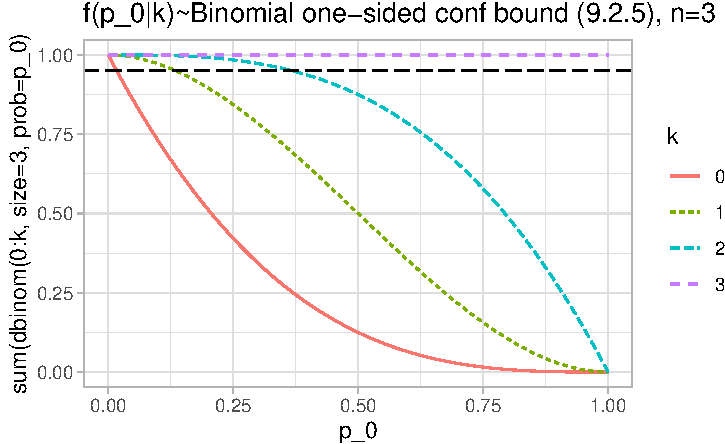
\includegraphics[width=1\linewidth]{class_notes_files/figure-latex/unnamed-chunk-6-1} \end{center}

\begin{itemize}
\item Note that we choose $k(p_0)$ for each $p_0$, so $k(p_0)$ is an integer-valued step-function of $p_0$:
\begin{itemize}
\item $f(0 | 0) = 1$, so $k(0) = 0$ and $f(p_0 | 0)$ remains above 1-$\alpha$ for an interval of values.
\item Then, at some point $f(p_0 | 0) = 1 - \alpha$ and for values of $p_0$ greater than this value, $f(p_0 | 0) < 1 - \alpha$. So, at this point, $k(p_0)$ increases to 1.
\item This pattern continues as $p_0$ increases and $k(p_0)$ increases one integer at a time: it is constant for a range of $p_0$, then it jumps to the next bigger integer.
\end{itemize}
\item since $k(p_0)$ is a nondecreasing function of $p_0$, this gives the lower confidence bound
\item solving the inequailities in (9.2.8) for $k(p_0)$ gives both the acceptance region of the test and the confidence set.
\begin{itemize}
\item for each $p_0: A(p_0) = \{t: t \leq k(p_0)\}$ where $k(p_0)$ satisfies (9.2.8)
\item for each value of $t$, the confidence set is $C(t) = \{ p_0: t \leq k(p_0)\}$.
\end{itemize}
\item How do we define this interval explicitly in terms of $p_0$?
\begin{itemize}
\item $k(p_0)$ is nondecreasing $\Rightarrow$ for a given observation $T=t, k(p_0) < t$ for all $p_0 < k^{-1}(t)$  where $k^{-1} (t)$ is some value we need to determine
\item confidence set is $C(t) = \{ p_0: t \leq k(p_0)\} = \{ p_0: p_0 > k^{-1}(t)\}$ where
$$k^{-1}(t) = \sup \left\{ p: \sum_{y=0}^{t-1} {n \choose y} p^{y} (1-p)^{n-y} \geq 1- \alpha \right\}$$
\end{itemize}
\item The problem of binomial confidence bounds was first treated by Clopper and Pearson (1934) who obtained answers similar to this for the two-sided interval.
\item Note this approach gives exact bounds. We instead could have used the normal approximation for large $n$ to get an approximate 95\% CI:
$$ \phat \pm z_{\alpha/2} \sqrt{\frac{\phat(1-\phat)}{n}}.$$
\end{itemize}

\subsubsection{Pivotal Quantities (9.2.2)}

Remember that in Example (9.1.6) the coverage probability of
\(\{aY, bY\}\) did not depend on the value of \(\theta\) while the
\(\{Y+c, Y+d\}\) interval did. This is because the coverage probability
of \(\{aY, bY\}\) could be expressed in terms of the quantity
\(Y/\theta\), a random variable whose distribution does not depend on
the parameter, a quantity known as a \emph{pivotal quantity}, or
\emph{pivot}.

We want to find a random variable depending on both the data and the
unknown parameter \(\theta\) whose distribution does not depend on
\(\theta\). Then, any probability statement about the pivotal quantity
will not depend on \(\theta\).

\noindent\textbf{Definition 9.2.6} A random variable
\(Q(\bX, \theta) = Q(\Xndots, \theta)\) is a \emph{pivotal quantity} or
\emph{pivot} if the distribution of \(Q(\bX, \theta)\) is independent of
all parameters. That is, if \(\bX \sim F(\bx |\theta)\), then
\(Q(\bX, \theta)\) has the same distribution for all values of
\(\theta\).

\begin{itemize}
\item $Q(\bx, \theta)$ will usually contain both parameters and statistics
\item for any set $\Asc$, $P_\theta(Q(\bX) \in \Asc)$ cannot depend on $\theta$
\end{itemize}

\noindent\textbf{Example: Gamma Pivot (9.2.8)} \(\Xndots \sim\)
exponential(\(\lambda\)). Then \(T = \sum X_i\) is a sufficient
statistic for \(\lambda\) and \(T\sim\) gamma(\(n,\lambda\)).

The gamma pdf is
\[\frac{1}{\Gamma(n) \lambda^{n}} t^{n-1} e^{-t/\lambda}\] and note that
\(t\) and \(\lambda\) appear together as \(t/\lambda\) and this gamma
distribution is a scale family.

Thus, if \(Q(T, \lambda) = 2T/\lambda\) and we let \(Y = 2T/\lambda\)
then by the transformation theorem,

\[g(t) = 2t/\lambda, \mbox{ and } g^{-1}(y) = \lambda y /2, \mbox{ and } \frac{d}{dy}g^{-1}(y) = \lambda/2\]
so
\[f_Y(y) = f_T(g^{-1}(y)) \left| \frac{d}{dy}g^{-1}(y)\right| = \frac{1}{\Gamma(n) \lambda^{n}} \left(\frac{\lambda y}{2}\right)^{n-1} e^{-(\lambda y /2)/\lambda} | \lambda/2| = \frac{1}{\Gamma(n)2^n} e^{-y/2}\]

which does not depend on \(\lambda\).

In fact, the quantity \(Q(T,\lambda) = 2T/\lambda\) is a pivot with a
gamma(\(n,2) = \chi^2_{2n}\) distribution:

\[Q(T,\lambda) \sim \mbox{ gamma}(n,\lambda(2/\lambda)) = \mbox{gamma}(n,2) = \chi^2_{2n}\]

Note that \(Q(T, \lambda) = T/\lambda\) is also a pivot with
distribution \(\Gamma(n,1)\).

\noindent\textbf{How to find the pivot?}

\begin{itemize}
\item There is no all purpose strategy for finding pivots.
\item  However, it is relatively easy to find pivots for location or scale parameters. In general, differences are pivotal for location parameters, while ratios (or products) are pivotal for scale problems.
\item looking at the distribution can give us a clue about the pivot, for instance $t/\lambda$ or $(\xbar - \mu)/\sigma$.
\item In general, suppose the pdf of a statistic $T, f(t|\theta)$ can be expressed in the form:
$$f(t| \theta) = g(Q(t,\theta))\left| \frac{\partial}{\partial t} Q(t, \theta)\right|$$
for some function $g$ and some monotone function $Q$ (monotone in $t$ for each $\theta$), then Theorem 2.1.5 can be used to show that $Q(T,\theta)$ is a pivot.
\end{itemize}

\noindent\textbf{Using the pivot:} If \(Q(\bX, \theta)\) is a pivot,
then for a specified value of \(\alpha\) we can find numbers \(a\) and
\(b\), which do not depend on \(\theta\) to satisfy:
\[P_\theta (a \leq Q(\bX, \theta) \leq b) \geq 1- \alpha.\] Then, for
each \(\theta_0 \in \Theta\),
\[ A(\theta_0) = \{\bx: a \leq Q(\bx, \theta_0) \leq b)\] is the
acceptance region for a level \(\alpha\) test of
\(H_0: \theta = \theta_0\). Using Theorem 9.2.2, we invert these tests
(for each \(\theta_0\)) to obtain:
\[C(\bx) = \{ \theta_0: a \leq Q(\bx, \theta_0) \leq b\},\] and
\(C(\bX)\) is a 1-\(\alpha\) confidence set for \(\theta\).

\noindent\textbf{Example: Continuation of Gamma Example 9.2.8} We
inverted a LRT to obtain the confidence interval for the mean
\(\lambda\) of an exponential(\(\lambda\)) pdf for
\(H_0: \lambda = \lambda_0\) versus \(H_1:\lambda \neq \lambda_0\).

Now we also see that if we have \(\Xndots\), we can define
\(T = \sum X_i\) and \(Q(T,\lambda) = 2T/\lambda \sim \chi^2_{2n}\)

If we choose constants \(a\) and \(b\) to satisfy
\(P(a \leq \chi^2_{2n} \leq b) = 1 - \alpha\) then
\[P_\lambda\left( a \leq \frac{2T}{\lambda} \leq b \right) = P_\lambda (a \leq Q(T,\lambda) \leq b) = P(a \leq \chi^2_{2n} \leq b) = 1 - \alpha.\]

Inverting the set
\(A(\lambda) = \{t: a \leq {2t/\lambda} \leq b\} \Rightarrow C(t) = \{ \lambda: 2t/b \leq \lambda \leq 2t/a\}\)
which is a \(1-\alpha\) confidence interval.

For example, if \(n=10\), then consulting a table of \(\chi^2\) cutoffs
gives a 95\% CI of \(\{\lambda: 2T/34.17 \leq \lambda \leq 2T/9.59\}.\)

\noindent\textbf{Example: Normal pivotal interval (9.2.10)}

This is a location problem. If we have
\(\Xndots \sim_{iid} \Nsc(\mu,\sigma^2)\), we know the distribution of
\((\Xbar - \mu)/(\sigma/\sqrt{n})\) is \(\Nsc(0,1)\) so that statistic
is a pivot.

if \(\sigma^2\) is known:
\[P\left(-a \leq \frac{\Xbar - \mu}{\sigma/\sqrt{n}} \leq a\right) = P(-a \leq Z \leq a),\]
\[ \Rightarrow C(\xbar) = \left\{ \mu: \xbar - a \frac{\sigma}{\sqrt{n}} \leq \mu \leq \xbar +  a \frac{\sigma}{\sqrt{n}}\right\}\]

If \(\sigma^2\) is unknown we use the sample estimate of \(\sigma\),
\(S\):
\[P\left(-a \leq \frac{\Xbar - \mu}{S/\sqrt{n}} \leq a\right) = P(-a \leq T_{n-1} \leq a),\]
\[ \Rightarrow C(\xbar) = \left\{ \mu: \xbar - t_{n-1,\alpha/2} \frac{s}{\sqrt{n}} \leq \mu \leq \xbar +  t_{n-1,\alpha/2} \frac{s}{\sqrt{n}}\right\}\]

Now if we want an interval estimate of \(\sigma\), we know that
\((n-1)^2S^2/\sigma^2 \sim \chi^2_{n-1}\) so \((n-1)^2S^2/\sigma^2\) is
also a pivot. Thus:
\[P\left(a \leq \frac{(n-1)S^2}{\sigma^2} \leq b \right) = P(a \leq \chi^2_{n-1} \leq b) = 1 - \alpha\]
\[\Rightarrow \left\{ \sigma: \sqrt{\frac{(n-1)s^2}{b}} \leq \sigma \leq  \sqrt{\frac{(n-1)s^2}{a}}\right\}.\]
We can choose \(a = \chi^2_{n-1,1-\alpha/2}\) and
\(b = \chi^2_{n-1,\alpha/2}\) so that the probability is equally split
between tails. However, the chi-square distribution is skewed so this is
not actually the optimal choice (we will explore this later in 9.3).

We constructed confidence intervals for \(\mu\) and \(\sigma\)
separately, but if we want a simultaneous confidence interval we can use
the Bonferroni Inequality (exercise 9.14).

\subsubsection{Pivoting the CDF}

\begin{itemize}
\item We saw that a pivot, $Q$, leads to a confidence set of the form:
$$C(\bx) = \{ \theta_0: a \leq Q(\bx, \theta_0) \leq b\}.$$
This will be an interval if $Q(\bx, \theta)$ is a monotone function of $\theta$ for every $\bx$.
\item If possible, constructing a confidence set based on a LRT will give a good (maybe not optimal) set. If it is too difficult to invert, the method of pivoting the CDF can be applied and will usually produce a reasonable set.
\end{itemize}

How to pivot the CDF?

\begin{itemize}
\item Suppose we base inference on a statistic, $T$, (ideally sufficient) for $\theta$, where $F_T(t|\theta)$ is the cdf for $T$. Suppose that $F_T(t|\theta)$ is monotone in $\theta$.
\item Note, if $F_T(t|\theta)$ is increasing (decreasing) in $\theta$ for every $t$ in the sample space of $T$, we say that $T$ is stochastically decreasing (increasing) in $\theta$.
\item Recall the Probability Integral Transformation, which tells us that the random variable $F_T(T|\theta)$ is Uniform(0,1), a pivot.
\item Thus, if $\alpha_1 + \alpha_2 = \alpha$, an $\alpha$-level acceptance region of the hypothesis $H_0: \theta = \theta_0$ is
$$\{t: \alpha_1 \leq F_T(t|\theta_0) \leq 1 - \alpha_2\},$$
with associated confidence set
$$\{ \theta: \alpha_1 \leq F_T(t|\theta) \leq 1 - \alpha_2\}.$$
\item To guarantee that the confidence set is an interval, we need to have $F_T(t|\theta)$ to be monotone in $\theta$
\end{itemize}

\noindent\textbf{Theorem 9.2.12 Pivoting a {\em continuous} cdf} Let
\(T\) be a statistic with continuous cdf \(F_T(t|\theta)\). Let
\(\alpha_1 + \alpha_2 = \alpha\) with \(0< \alpha < 1\) be fixed values.
Suppose that for each \(t \in \Tsc\), the functions \(\theta_{L}(t)\)
and \(\theta_{U}(t)\) can be defined as follows

\begin{enumerate}
\def\labelenumi{\roman{enumi}.}
\item
  If \(F_t(t|\theta)\) is a decreasing function of \(\theta\) for each
  \(t\), define \(\theta_{L}(t)\) and \(\theta_{U}(t)\) by
  \[F_T(t|\theta_{U}(t)) = \alpha_1, \,\, F_T(t|\theta_{L}(t))  = 1 - \alpha_2.\]
\item
  If \(F_T(t|\theta)\) is an increasing function of \(\theta\) for each
  \(t\), define \(\theta_{L}(t)\) and \(\theta_{U}(t)\) by
  \[F_T(t|\theta_{U}(t)) = 1-\alpha_2, \, \, F_T(t|\theta_{L}(t))  = \alpha_1.\]
\end{enumerate}

Then the random interval \([\theta_{L}(t),\theta_{U}(t)]\) is a
\(1-\alpha\) confidence interval for \(\theta\).

\noindent\textbf{Proof (of part (i))}:

First recall the general idea behind the proof of the Probablity
Integral Transform, where \(Y= F_T(T)\):
\[F_Y(y) = P(Y\leq y) = P(F_T(T) \leq y) = P(T \leq F_T^{-1}(y)) = F_T(F_T^{-1}(y)) = y\]
So \(Y\) has cdf \(F_Y(y) = y\), which is the cdf of Uniform(0,1).

Now, assume we have constructed the 1-\(\alpha\) acceptance region:
\[\{t: \alpha_1 \leq F_T(t|\theta_0) \leq 1 - \alpha_2\}.\]

Since \(F_T(T|\theta)\) is decreasing in \(\theta\) for all \(t\)
\(\Rightarrow\)
\[F_T(t|\theta) < \alpha_1 \Leftrightarrow \theta > \theta_U(t).\]
Similarly
\[F_T(t|\theta) > 1 - \alpha_2 \Leftrightarrow \theta < \theta_L(t)\]
Hence: \begin{align*}
P(\theta_L(T) \leq \theta \leq \theta_U(T)) & = 1 - \{ P(\theta > \theta_U(T)) + P(\theta < \theta_L(T))\}\\
&= 1 - \{P_\theta(F_T(T|\theta) < \alpha_1) + P_\theta(F_T(T|\theta) > 1- \alpha_2)\}\\
&= 1 - (\alpha_1 + \alpha_2) = 1- \alpha
\end{align*}

The proof of part (ii) is similar.

\textbf{Notes:}

\begin{itemize}
\item Note: we can assume $\alpha_1 = \alpha_2 = \alpha/2$ but this may not be optimal split.
\item If we want a one-sided interval we can choose $\alpha_1 = 0$ or $\alpha_2 = 0$.
\end{itemize}

\noindent\textbf{Example 9.2.13 Location exponential interval}

Let \(\Xndots \sim_{iid} f(x|\mu) = e^{-(x-\mu)}I_{[\mu,\infty)}(x).\)
Then \(Y = min\{\Xndots\} = X_{(1)}\) is sufficient for \(\mu\) with pdf
\(f_Y(y|\mu) = ne^{-n(y-\mu)} I_{[\mu,\infty)}(y).\)

We have a decreasing function so we can fix \(\alpha\) and define
\(\mu_L(y)\) and \(\mu_U(y)\) to satisfy: \begin{align*}
F_Y(y|\mu_U(y)) = \frac{\alpha}{2}, \mbox{ and }&  F_Y(y|\mu_L(y)) = 1-  \frac{\alpha}{2}\\
\int_{\mu_U(y)}^y ne^{-n(u - \mu_U (y))} du  = \frac{\alpha}{2}, \mbox{ and }&  
\int_{y}^\infty ne^{-n(u - \mu_L (y))} du  = \frac{\alpha}{2}
\end{align*}

Evaluate the integrals:
\[1 - e^{-n(y-\mu_U(y))} = \frac{\alpha}{2},  \mbox{ and } e^{-n(y-\mu_L(y))} = \frac{\alpha}{2}\]
then solve:
\[ \mu_U(y) = y + \frac{1}{n} \log\left( 1 - \frac{\alpha}{2}\right),\mbox{ and }\mu_L(y) = y + \frac{1}{n} \log\left( \frac{\alpha}{2}\right)\]
So this random interval is a 1-\(\alpha\) confidence interval for
\(\mu\):
\[C(Y) = \left\{ \mu: Y + \frac{1}{n}\log\left( \frac{\alpha}{2}\right) \leq \mu \leq Y +\frac{1}{n} \log\left( 1 - \frac{\alpha}{2}\right)\right\}\]

\begin{itemize}
\item Note that we only need to solve the CDF equations for the value of the statistics actually observed.
\item We may solve them analytically or numerically.
\item Now consider the discrete case:
\end{itemize}

\noindent\textbf{Theorem 9.2.14 Pivoting a {\em discrete} cdf} Let \(T\)
be a discrete statistic with cdf
\(F_T(t|\theta) = P(T \leq t | \theta)\). Let
\(\alpha_1 + \alpha_2 = \alpha\) with \(0< \alpha < 1\) be fixed values.
Suppose that for each \(t \in \Tsc\), the functions \(\theta_{L}(t)\)
and \(\theta_{U}(t)\) can be defined as follows

\begin{enumerate}
\def\labelenumi{\roman{enumi}.}
\item
  If \(F_t(t|\theta)\) is a decreasing function of \(\theta\) for each
  \(t\), define \(\theta_{L}(t)\) and \(\theta_{U}(t)\) by
  \[P(T \leq t|\theta_{U}(t)) = \alpha_1, \,\, P(T \geq t|\theta_{L}(t))  = \alpha_2.\]
\item
  If \(F_T(t|\theta)\) is an increasing function of \(\theta\) for each
  \(t\), define \(\theta_{L}(t)\) and \(\theta_{U}(t)\) by
  \[P(T \geq t|\theta_{U}(t)) = \alpha_1, \, \, P(T \leq t|\theta_{L}(t))  = \alpha_2.\]
\end{enumerate}

Then the random interval \([\theta_{L}(t),\theta_{U}(t)]\) is a
\(1-\alpha\) confidence interval for \(\theta\).

\textbf{Proof}: See book.

\noindent\textbf{Example 9.2.15 Poisson Interval Estimator} Let
\(\Xndots \sim_{iid}\) Poisson(\(\lambda\)) and define
\(T = \sumin X_i.\) Then \(T\) is sufficient for \(\lambda\) and
\(Y\sim\) Poisson(\(n\lambda\)).

Let \(\alpha_1 = \alpha_2 = \alpha/2\) in the above theorem. The cdf is
a decreasing function of \(\lambda\) for each \(t\) since the cdf is
\[P(T\leq t | \lambda) = \sum_{k=0}^{t} e^{-n\lambda}\frac{(n\lambda)^k}{k!}\]

and has a negative derivative for all values of \(\lambda>0\):
\[\frac{d}{d\lambda} P(T\leq t | \lambda) = \sum_{k=0}^{t} -ne^{-n\lambda}\frac{kn^k\lambda^{(k-1)}}{k!}<0\]

So, if \(T = t_0\) is observed, we need to solve \(\lambda\) in the
equations to obtain the lower and upper limits \(\lambda_L\) and
\(\lambda_U\): \begin{equation*}
P(T\leq t_0 | \lambda_U)= \sum_{k=0}^{t_0} e^{-n\lambda_U}\frac{(n\lambda_U)^k}{k!} = \frac{\alpha}{2} \mbox{ and } 
P(T\geq t_0 | \lambda_L) = \sum_{k=t_0}^{\infty} e^{-n\lambda_L}\frac{(n\lambda_L)^k}{k!} = \frac{\alpha}{2} 
\tag{9.2.16}
\end{equation*}

How do we solve these equations? First, recall: If \(G\) is a
gamma\((a,b)\) random variable, where \(a\) is an integer, then for any
\(g\), \[P(G \leq g) = P(H\geq a) \mbox{ where } H\sim Poisson(g/b).\]
Hence,

\begin{align*}
\alpha/2 & =  \sum_{k=0}^{t_0} e^{-n\lambda_U}\frac{(nk)^k}{k!} \\
& =P(Y \leq t_0 | \lambda_U) \\
&= P(Pois(n\lambda_U) < t_0 + 1)\\
&= 1 - P(Pois(n\lambda_U) \geq t_0 + 1)\\
&= 1 - P(Gamma(t_0 + 1, 2) \leq 2n\lambda_U)\\
& = 1 - P(\chi^2_{2(t_0+1)}\leq 2n\lambda_U)\\
& = P(\chi^2_{2(t_0+1)}> 2n\lambda_U)\\
\end{align*} Then solving for the critical value:
\[2n\lambda_U = \chi^2_{2(t_0+1),\alpha/2}\] Solving for \(\lambda_U\):
\[\lambda_U = \frac{1}{2n}\chi^2_{2(t_0 + 1),\alpha/2}\]

Applying the identity to the other equation in 9.2.16 yields:
\[\frac{\alpha}{2} = P(\chi^2_{2t_0} < 2n\lambda_L) \Rightarrow 1-\frac{\alpha}{2} = P(\chi^2_{2t_0} \geq 2n\lambda_L).\]
Then solving for the critical value:
\[2n\lambda_L = \chi^2_{2t_0,1-\alpha/2}\]

and so \[\lambda_L = \frac{1}{2n}\chi^2_{2t_0, 1-\alpha/2}\]

and a \(1-\alpha\) confidence interval for \(\lambda\) is:
\[\left\{ \lambda: \frac{1}{2n} \chi^2_{2t_0,1-\alpha/2} \leq \lambda \leq \frac{1}{2n}\chi^2_{2(t_0 + 1),\alpha/2}\right\}.\]

Suppose \(t_0 = 4\) and \(\alpha = 0.05\) and \(n=20\), then the
confidence interval is:

\begin{Shaded}
\begin{Highlighting}[]
\NormalTok{nn =}\StringTok{ }\DecValTok{20}
\NormalTok{t0 =}\StringTok{ }\DecValTok{4}
\NormalTok{alpha =}\StringTok{ }\FloatTok{.05}

\NormalTok{lambda_l <-}\StringTok{ }\KeywordTok{qchisq}\NormalTok{(}\DataTypeTok{p=}\DecValTok{1}\OperatorTok{-}\NormalTok{alpha}\OperatorTok{/}\DecValTok{2}\NormalTok{, }\DataTypeTok{df=}\DecValTok{2}\OperatorTok{*}\NormalTok{t0, }\DataTypeTok{lower.tail =} \OtherTok{FALSE}\NormalTok{)}\OperatorTok{/}\NormalTok{(}\DecValTok{2}\OperatorTok{*}\NormalTok{nn)}
\NormalTok{lambda_u <-}\StringTok{ }\KeywordTok{qchisq}\NormalTok{(}\DataTypeTok{p=}\NormalTok{alpha}\OperatorTok{/}\DecValTok{2}\NormalTok{, }\DataTypeTok{df=}\DecValTok{2}\OperatorTok{*}\NormalTok{(t0}\OperatorTok{+}\DecValTok{1}\NormalTok{), }\DataTypeTok{lower.tail =} \OtherTok{FALSE}\NormalTok{)}\OperatorTok{/}\NormalTok{(}\DecValTok{2}\OperatorTok{*}\NormalTok{nn)}
\KeywordTok{c}\NormalTok{(lambda_l, lambda_u)}
\end{Highlighting}
\end{Shaded}

\begin{verbatim}
#> [1] 0.05449327 0.51207943
\end{verbatim}

The 95\% CI for \(\lambda\) is: {[}0.054, 0.512{]}

For \(n=100\):

\begin{Shaded}
\begin{Highlighting}[]
\NormalTok{nn =}\StringTok{ }\DecValTok{100}
\NormalTok{t0 =}\StringTok{ }\DecValTok{4}
\NormalTok{alpha =}\StringTok{ }\FloatTok{.05}

\NormalTok{lambda_l <-}\StringTok{ }\KeywordTok{qchisq}\NormalTok{(}\DataTypeTok{p=}\DecValTok{1}\OperatorTok{-}\NormalTok{alpha}\OperatorTok{/}\DecValTok{2}\NormalTok{, }\DataTypeTok{df=}\DecValTok{2}\OperatorTok{*}\NormalTok{t0, }\DataTypeTok{lower.tail =} \OtherTok{FALSE}\NormalTok{)}\OperatorTok{/}\NormalTok{(}\DecValTok{2}\OperatorTok{*}\NormalTok{nn)}
\NormalTok{lambda_u <-}\StringTok{ }\KeywordTok{qchisq}\NormalTok{(}\DataTypeTok{p=}\NormalTok{alpha}\OperatorTok{/}\DecValTok{2}\NormalTok{, }\DataTypeTok{df=}\DecValTok{2}\OperatorTok{*}\NormalTok{(t0}\OperatorTok{+}\DecValTok{1}\NormalTok{), }\DataTypeTok{lower.tail =} \OtherTok{FALSE}\NormalTok{)}\OperatorTok{/}\NormalTok{(}\DecValTok{2}\OperatorTok{*}\NormalTok{nn)}
\KeywordTok{c}\NormalTok{(lambda_l, lambda_u)}
\end{Highlighting}
\end{Shaded}

\begin{verbatim}
#> [1] 0.01089865 0.10241589
\end{verbatim}

The 95\% CI for \(\lambda\) is: {[}0.011, 0.102{]}

Similar derivations can be done for negative binomial and binomial
distributions. The graph of coverage probabilities for binomial
confidence intervals is given in Figure 9.2.5.

\subsection{Methods of Evaluating Interval Estimators (9.3)}

What makes a good interval? Small size and large coverage

\begin{itemize}
    \item $(-\infty,\infty)$ has coverage probability 1
    \item in order to optimize, need to know how to measure these quantities
    \item sometimes a function of the parameter
    \item coverage usually measured by confidence coefficient (infimum of converge probabilities)
    \item size of an interval usually means length
    \end{itemize}

\noindent\textbf{Example 9.3.1 Optimimizing Length} Let
\(\Xndots \sim_{iid} \Nsc(\mu,\sigma^2)\) where \(\sigma\) is known.

Using the pivotal quantity
\[Z = \frac{\Xbar - \mu}{\sigma/\sqrt{n}} \sim \Nsc(0,1)\] which has a
distribution that does not depend on \(\mu\), we know (section 9.2.2
Pivotal Quantities) that if we choose \(a\) and \(b\) such that:
\(P(a \leq Z \leq b) =1-\alpha\) we will have the \(1-\alpha\)
confidence interval
\[C(\mu) = \left\{ \mu: \xbar - b \frac{\sigma}{\sqrt{n}} \leq \mu \leq \xbar - a \frac{\sigma}{\sqrt{n}}\right\}.\]

This gives \(1-\alpha\) coverage, and a \(1-\alpha\) confidence
coefficient.

How can we minimize the length?

\[length(C(\mu)) = \xbar - a \frac{\sigma}{\sqrt{n}} - \xbar + b \frac{\sigma}{\sqrt{n}} =  \frac{(b-a)\sigma}{\sqrt{n}}\]

So we need to minimize \(b-a\).

In Example 9.2.1 we chose \(a = -z_{\alpha/2}\) and \(b = z_{\alpha/2}\)
but we did not consider optimality. We can take any other combination of
values \(a=z_{a}\) and \(b=z_{b}\) and such that
\(P(a \leq Z \leq b) = z_{b} + 1 - z_{a} = 1-\alpha\), and in fact if we
let \(\alpha = 0.1\) then we have many options for 90\% intervals (see
table in C\&B, page 441).

Looking at those examples we see that splitting the probability
\(\alpha\) equally is an optimal strategy, as \(a = -1.65 = -z_{.05}\)
and \(b=1.65 = z_{.05}\) gives the shortest interval.

\begin{itemize}
\item splitting $\alpha$ equally does not always give the optimal length
\item in the previous case, the height of the pdf is the same at $-z_{\alpha/2}$ and $z_{\alpha/2}$
\item we can prove a theorem that demonstrates a general version of this fact for a unimodal distribution
\end{itemize}

\noindent\textbf{Theorem 9.3.2} Let f(x) be a unimodal pdf. If the
interval \([a,b]\) satisfies

\begin{enumerate}
\item[(i)] $\int_{a}^{b} f(x) dx = 1-\alpha$
\item[(ii)] $f(a) = f(b) > 0,$ and
\item[(iii)] $a \leq x^* \leq b$ where $x^*$ is a mode of $f(x)$
\end{enumerate}

then \([a,b]\) is the shortest among all intervals that satisfy \((i)\).

\def\aprime{a^\prime}
\def\bprime{b^\prime}

\noindent\textbf{Proof (skip details in class; uses mean value theorem to show coverage outside of peak is lower):}
Let \([a^\prime,b^\prime]\) be any interval shorter than our interval so
\(b^\prime- a^\prime< b - a\). We will show that this implies lower
coverage \(\int_{a^\prime}^{b^\prime} f(x) dx < 1-\alpha\). We will
prove this for \(a^\prime\leq a\).

Case \(b^\prime\leq a\):
\(\Rightarrow a^\prime\leq b^\prime\leq a \leq x^{*}\) and
\begin{align*}
\Rightarrow \int_{a^\prime}^{b^\prime}f(x)dx &\leq f(b^\prime)(b^\prime-a^\prime) \quad (x \leq b^\prime\leq x^* \Rightarrow f(x) \leq f(b^\prime))\\
&\leq f(a) (b^\prime- a^\prime) \quad (b^\prime\leq a \leq x^* \Rightarrow f(b^\prime) \leq f(a))\\
&< f(a) (b-a) \quad (b^\prime- a^\prime< b-a \mbox{ and } f(a)>0)\\
& \leq \int_{a}^{b} f(x) dx \quad ((ii) (iii) \mbox{ and unimodality } \Rightarrow f(x) \geq f(a) \mbox{ for } a \leq x \leq b)\\
= 1-\alpha
\end{align*}

Case \(b^\prime> a:\)

If \(b^\prime\geq b \Rightarrow b^\prime- a^\prime\geq b-a\) which is
false, so \(b^\prime< b\) and more specifically
\(\Rightarrow a^\prime\leq a < b^\prime< b\).

\begin{align*}
\Rightarrow \int_{a^\prime}^{b^\prime}f(x)dx &= \int_{a}^{b}f(x)dx + \left[\int_{a^\prime}^{a}f(x)dx - \int_{b^\prime}^{b}f(x)dx \right] \\
&=(1-\alpha) + \left[\int_{a^\prime}^{a}f(x)dx - \int_{b^\prime}^{b}f(x)dx \right] \\
&= (1-\alpha) + B
\end{align*}

Is B negative?

From the unimodality of \(f\),
\(\Rightarrow a^\prime\leq a < b^\prime< b\), and (ii) and arguments
similar to above we have:

\[\int_{a^\prime}^{a}f(x)dx \leq f(a) (a-a^\prime) \mbox{ and } \int_{b^\prime}^{b}f(x)dx \geq f(b) (b-b^\prime)\]

Thus, \begin{align*}
B &= \int_{a^\prime}^{a}f(x)dx - \int_{b^\prime}^{b}f(x)dx\\
&\leq f(a) (a-a^\prime) - f(b) (b-b^\prime)\\
&= f(a) [ (a-a^\prime) - (b- b^\prime)] \quad (f(a) = f(b))\\
&= f(a) [(b^\prime- a^\prime) - (b-a)]\\
&<0 \quad ((b^\prime- a^\prime) < (b-a) \mbox{ and } f(a) >0)
\end{align*}

\noindent\textbf{Note} The form of likelihood regions has optimal
construction by this theorem. Recall (re-read example 9.2.3 and
discussion)

\begin{itemize}
\item The region obtained by inverting the LRT of $H_0: \theta = \theta_0$ versus $H_1: \theta \neq \theta_0$ is of the form:
$$\mbox{accept } H_0 \mbox{ if } \frac{\Lsc(\theta_0 |\bx)}{\Lsc(\thetahat|\bx)} \leq k(\theta_0)$$
with the resulting confidence region
$$\{\theta : \Lsc(\theta|\bx) \geq k^\prime(\bx,\theta)\},$$
for some function $k^\prime$ that gives $1-\alpha$ confidence
\item In some cases (i.e. Normal and Gamma distribution) the function $k^\prime$ will not depend on $\theta$
\item In this case the likelihood region is the set containing $\theta$ for which the likelihood is highest
\item Now, we know we have the optimal length if $f(a) = f(b)$ for a unimodal distribution
\end{itemize}

\noindent\textbf{Example 9.3.3 Optimizing expected length} For normal
intervals of \(\mu\) with unknown variance based on the pivot
\(\frac{\Xbar - \mu}{S/\sqrt{n}}\) we know that the shortest length
\(1-\alpha\) confidence interval of the form
\[\left[\xbar - b\frac{s}{\sqrt{n} }\leq \mu \leq \xbar - a\frac{s}{\sqrt{n}}\right]\]
has \(a= -t_{n-1,\alpha/2}\) and \(b=t_{n-1,\alpha/2}.\) The interval
length is a function of \(s\), with general form
\[length(x) = (b-a)\frac{s}{\sqrt{n}}.\]

We can instead consider the criterion of \emph{expected length} and seek
an interval with \(1-\alpha\) coverage that minimizes
\[E_{\sigma}(length(S)) = (b-a)\frac{E_{\sigma} S}{\sqrt{n}} = (b-a) c(n) \frac{\sigma}{\sqrt{n}},\]
(where the quantity \(c(n)\) is a constant dependent only on \(n\)) then
Theorem 9.3.2 applies and the choice \(a = -t_{n-1,\alpha/2}\) and
\(b=t_{n-1,\alpha/2}\) again gives us an optimal interval.

\textbf{Example 9.3.4: Shortest pivotal interval (scale parameter)} Let
\(X \sim gamma(k,\beta)\). Then \(Y=X/\beta\) is a pivot, with
\(Y \sim gamma(k,1)\), so we can get a confidence interval by finding
constants \(a\) and \(b\) to satisfy \[P(a \leq Y \leq b) = 1-\alpha\]

However, if we apply Theorem 9.3.2 we won't have the shortest confidence
interval:

If we choose \(a\) and \(b\) such that \(P(a \leq Y \leq b) = 1-\alpha\)
and \(f_Y(a) = f_Y(b)\) then the interval on \(\beta\) is of the form:
\[RR = \left\{ x: a \leq \frac{x}{\beta} \leq b \right\} \Rightarrow\]
\[CI = \left\{ \beta: \frac{x}{b} \leq \beta \leq\frac{x}{a}\right\} \Rightarrow length(CI) =  \left(\frac{1}{a} - \frac{1}{b}\right) x\]
which is proportional to \((1/a) - (1/b)\) and not to \(b-a\).

We can modify Theorem 9.3.2 to apply here.

Condition (a) in Thm 9.3.2 defines \(b\) as a function of \(a\), so call
it \(b(a)\). We must solve the following constrained minimization
problem:

\begin{itemize}
\tightlist
\item
  \textbf{Minimize, with respect to a:} \(\frac{1}{a} - \frac{1}{b(a)}\)
\item
  \textbf{Subject to} \(\int_{a}^{b(a)} f_Y(y) dy = 1-\alpha\)
\end{itemize}

Differentiate the first equation with respect to \(a\) and setting it
equal to 0 yields \[\frac{db}{da} = \frac{b^2}{a^2}\] Differentiate the
second equation which must equal 0 and substitute this in gives
\[f(b)b^2 = f(a) a^2\]

\begin{itemize}
\item equations like these arise in interval estimate of the variance of a normal distribution
\item the above equations define not he shortest {\em overall} interval but the shortest {\em pivotal} interval, that is, the shortest interval based on the pivot $X/\beta$
\item this result can be generalized using the Neyman-Pearson Lemma (Exercise 9.43)
\end{itemize}

\subsubsection{Bayesian Intervals}

\begin{itemize}
\item We say that the confidence interval {\em covers} the parameter, not that the parameter is {\em is inside} the interval. This denotes that the random quantity is the interval, not the parameter.
\item In a Bayesian setting, the parameter is indeed random and we may say that the parameter is inside an interval with some probability, not 0 or 1.
\item All Bayesian claims of coverage are made with respect to the posterior distribution of the parameter
\item Bayesian set estimates are referred to as {\em credible sets} rather than confidence sets.
\item If $\pi(\theta|\bx)$ is the posterior distribution of $\theta$ given $\bX = \bx$, then for any set $A \subset \Theta$, the credible probability of $A$ is:
$$P(\theta \in A |\bx) = \int_A \pi(\theta|\bx) d\theta,$$
and $A$ is a {\em credible set} for $\theta$. If $\pi$ is a pmf, we replace integrals with sums.
\item Now the parameter is random and the interval is fixed (given the data).
\end{itemize}

\noindent\textbf{Example 9.2.16 Poisson credible set} We wish to
construct a credible set for the above Poisson example 9.2.15.

Let \(\Xndots \sim_{iid} Poisson(\lambda)\) and assume \(\lambda\) has a
Gamma prior pdf, \(\lambda \sim\) gamma(\(a,b\)).

The posterior pdf of \(\lambda\) is then (after applying Bayes' Rule):
\[\pi(\lambda | \sum X  = \sum x) = \mbox{gamma}(a + \sum x, [n+(1/b)]\inv\]

We can form a credible set for \(\lambda\) in many ways. One simple way
is to split \(\alpha\) equally between the upper and lower tails:
\[P(\lambda < \lambda_L(t) |T = t) = P(\lambda > \lambda_U(t) | T = t) = \alpha/2\]

Using the fact that if \(Y\sim Gamma(\alpha,\beta)\) then
\(2Y/\beta \sim \chi^2_{2\alpha}\), it follows that
\(\frac{2(nb+1)}{b}\lambda \sim \chi^2_{2(a+\sum x_i)}\) assuming \(a\)
is an integer:
\[\alpha/2 = P(\lambda < \lambda_L(t) | T = t) = P\left(\frac{2\lambda}{b/(bn+1)} < \frac{2\lambda_L(t)}{b/(bn+1)} | T = t\right) = P\left(\chi^2_{2(a+t)} <\frac{2\lambda_L(t)}{b/(bn+1)} t\right)
\] so
\[ \frac{2\lambda_L(t)}{b/(bn+1)} = \chi^2_{2(a+t),1-\alpha/2} \Rightarrow \lambda_L(t) = \frac{b}{2(bn+1}\chi^2_{2(a+t),1-\alpha/2}\]

Thus a \(1-\alpha\) credible interval is:
\[ \left\{\lambda: \frac{b}{2(bn+1)}\chi^2_{2(a+t),1-\alpha/2} \leq \lambda \leq  \frac{b}{2(bn+1)}\chi^2_{2(a+t),\alpha/2} \right\}\]

If we take \(a = b = 1\), the \(1-\alpha\) credible interval becomes:
\[\left( \frac{1}{2(n+1) }\chi^2_{2(1+t),1-\alpha/2},\frac{1}{2(n+1) }\chi^2_{2(1+t),\alpha/2}\right)\]
while the confidence interval (frequentist) we obtained earlier was:
\[\left[ \frac{1}{2n }\chi^2_{2(1+t),1-\alpha/2},\frac{1}{2n }\chi^2_{2(1+t),\alpha/2}\right]\]

\textbf{Notes:}

\begin{itemize}
\item In this case (see Figure 9.2.3), the credible set has somewhat shorter intervals than the confidence interval, and the upper endpoints are closer to 0. This reflects the prior, which is pulling the intervals toward 0.
\item We can now ask, what is the probability of getting data $(\bX)$ for which the credible interval contains the parameter $\lambda$? We can show this goes to 0 as $\lambda \to \infty$.
\item Likewise, we can ask what is the posterior probability that the confidence interval contains the true parameter? This also goes to 0 as $\sumin X_i \to \infty$, unless $b  = 1/n$.
\item Using Bayesian criteria for frequentist intervals or frequentist criteria for Bayesian intervals can result in poor calculated performance. That is, Bayesian intervals don't necessarily have good frequentist properties and frequentist intervals don't necessarily have good Bayesian properties.
\end{itemize}

\newpage

\hypertarget{basic-concepts-of-random-samples-cb-chapter-5}{%
\section{Basic Concepts of Random Samples (C\&B Chapter
5)}\label{basic-concepts-of-random-samples-cb-chapter-5}}

\hypertarget{random-sample-from-an-infinitely-large-population}{%
\subsection{Random sample from an infinitely large
population}\label{random-sample-from-an-infinitely-large-population}}

Recall the definition of a random sample (or, \(iid\) random sample):

\textbf{Definition} The random variables \(\Xndots\) are called a
\emph{random sample} from the population \(f_X(x)\) if

\begin{enumerate}
\item $X_i, \ldots, X_n$ are mutually independent
\item The marginal pdf (pmf) of each $X_i$ is the same function $f_X(x)$
\end{enumerate}

\hypertarget{finite-population-sampling-we-wont-use-this-in-bsta-552-unless-we-have-time-to-talk-about-bootstrapping}{%
\subsection{Finite population sampling (we won't use this in BSTA 552
unless we have time to talk about
bootstrapping)}\label{finite-population-sampling-we-wont-use-this-in-bsta-552-unless-we-have-time-to-talk-about-bootstrapping}}

When we say ``random sample'' we mean that we are sampling from an
infinite population. We can alternatively sample from a \emph{finite}
population, say \(\{x_1, x_2, \ldots, x_N\}\) where \(N< \infty\)
denotes the size of the population. In this case, we are drawing a
sample \(X^*_1, X^*_2, \ldots, X^*_n\) from the set
\(\{x_1, x_2, \ldots, x_N\}\). There are two options for this type of
(re-)sampling:

\begin{enumerate}
\item Simple random sample {\em with replacement}
\begin{itemize}
\item Each value $x_i$ is "replaced" after it is selected (every time you draw a number from a hat you put it back in the hat before drawing the next value)
\item Each sample $X^*_i$ has a discrete uniform distribution with equal probability mass $1/N$ on each of the values $x_1, x_2, \ldots, x_N$.
\item The $X^*_i$'s are mutually independent because the process of choosing each $x^*_i$ is the same, regardless of the values that are chosen for any of the other variables $\Rightarrow$ $X^*_1, X^*_2, \ldots, X^*_n$ are $iid$.
\item This type of sampling is the basis of the resampling technique known as {\em bootstrapping}
\end{itemize}
\item Simple random sample {\em without replacement}
\begin{itemize}
\item When sampling from the set $\{x_1, x_2, \ldots, x_N\}$, each value $x_i$ is not replaced after it is selected (do not put the number back in the hat before choosing the next value)
\item The $X^*_i$'s are no longer mutually independent because the probability that $X^*_i$ is equal to some value depends on all the other values selected before it, for instance:
  \begin{align*}
P(X^*_1 = x_i) &= 1/N\\
P(X^*_2 = x_i | X^*_1=x_i) &= 0\\
\mbox{however, if } x_j \neq x_i, \mbox{ then } P(X^*_2 = x_i | X^*_1=x_j) &= 1/(N-1).
\end{align*}
\item However, the $X^*_i$'s are identically distributed (they have the same marginal distributions, see pg 210 for explanation).
\item If the population size $N$ is "large" then this type of sampling is approximately equal to sampling from an infinite population, and the samples are "nearly independent" in that the conditional distributions are very close to the marginal distributions.
\end{itemize}
\end{enumerate}

\hypertarget{convergence-concepts-foundations-needed-for-chapter-10}{%
\section{Convergence concepts (foundations needed for Chapter
10)}\label{convergence-concepts-foundations-needed-for-chapter-10}}

In Chapter 10, we will be discussing convergence of statistics to
parameters and also asymptotic distributions of statistics. So first, we
define what we mean by ``convergence'' and ``asymptotics''.

\begin{itemize}
\tightlist
\item
  Asymptotic theory examines what happens to sample quantities
  (i.e.~statistics) when the sample size approaches infinity.
\item
  There are three main types of convergence: convergence in probability,
  convergence in distribution, and convergence almost surely. We will
  only discuss the first two in this course.
\end{itemize}

\hypertarget{convergence-in-probability-consistency}{%
\subsection{Convergence in probability
(consistency)}\label{convergence-in-probability-consistency}}

\noindent\textbf{Definition 5.5.1 Convergence in probability:} A
sequence of random variables, \(Y_1, Y_2, \ldots,\) converges in
probability to a random variable \(Y\) if, for every small number
\(\delta > 0\),
\[ \lim_{n\to \infty} P(|Y_n - Y| \geq \delta) = 0 \mbox{ or, equivalently, } \lim_{n\to\infty} P(|Y_n - Y|< \delta) = 1\]

We also define convergence in probability to a constant the same way. A
sequence of random variables, \(Y_1, Y_2, \ldots,\) converges in
probability to a constant value \(\theta\) if, for every \(\delta > 0\),
\[ \lim_{n\to \infty} P(|Y_n - \theta| \geq \delta) = 0 \mbox{ or, equivalently, } \lim_{n\to\infty} P(|Y_n - \theta|< \delta) = 1\]

\begin{itemize}
\tightlist
\item
  For notation, we often write convergence in probability as:
  \(Y_n \to_p Y\) or \(Y_n \to_p \theta\)
\item
  Convergence in probability means that as \(n\) approaches infinity the
  random variable \(Y_n\) becomes arbitrarily close to the random
  variable \(Y\) or the constant \(\theta\).
\item
  In Chapter 10, we will be using convergence in probability with a
  sequence of random variables based on our data:
  \(W_n = W_n(X_1, \ldots, X_n)\) such as \(W_n = \sum_{i=1}^n X_i\) or
  \(W_n = \Xbar_n\). Remember, this is called a \emph{statistic}. We are
  also usually more concerned with convergence in probability of a
  statistic to a constant value (as opposed to a random variable).
\item
  Note we have added a subscript \(n\) to \(\Xbar\) here since the
  distribution of \(\Xbar\) depends on \(n\).
\item
  In Chapter 10, we call convergence in probability of a statistic (or a
  sequence of the same sample quantity such as \(\Xbar_n\)) to a
  parameter \(\theta\) \emph{consistency} of a statistic.
\end{itemize}

It is often easiest to prove convergence in probability using:

\textbf{Chebychev's Inequality (Theorem 3.6.1):} Let \(X\) be a random
variable and let \(g(x)\) be a nonnegative function. Then, for any
\(r> 0\), \[P(g(X) \geq r) \leq \frac{E[g(X)]}{r^2}.\]

To use this in the above definition of convergence in probability, we
first square the difference to get rid of the absolute value and then
use Chebychev's Inequality:
\[P(|Y_n - Y| \geq \epsilon) = P((Y_n - Y)^2 \geq \epsilon^2) \leq \frac{E[(Y_n - Y)^2]}{\epsilon^4}.\]
so we see that the probability that the distance \(|Y_n - Y|\) or
\(|Y_n - \theta|\) is arbitrarily large can be bound above by
\(E[(Y_n - Y)^2]\) or \(E[(Y_n - \theta)^2]\). Hence, if
\(E[(Y_n - Y)^2]\) goes to 0 as \(n \to \infty\) then we have
convergence in probability to \(Y\). We will see an example of this in
the proof of the following theorem.

A special and often used example of convergence in probability is the
Weak Law of Large Numbers for \(W_n = \Xbar_n\):

\textbf{Weak Law of Large Numbers (WLNN, Theorem 5.5.2):} Let
\(X_1, X_2, \ldots\) be \(iid\) random variables with \(E X_i = \mu\)
and \(\Var X_i = \sigma^2 < \infty\). Define
\[\Xbar_n = n\inv\sumin X_i\]

Then, for every \(\epsilon > 0\):
\[\lim_{n\to\infty} P(|\Xbar_n - \mu| < \epsilon) = 1;\] that is,
\(\Xbar_n\) converges in probability to \(\mu\).

\noindent\textbf{Proof of WLLN:} We can prove this using Chebychev's
inequality.
\[P(|\Xbar_n - \mu| \geq \epsilon) = P((\Xbar_n - \mu)^2 \geq \epsilon^2) \leq \frac{E(\Xbar_n - \mu)^2}{(\epsilon^2)^2} = 
  \frac{\Var \Xbar_n}{(\epsilon^2)^2} = \frac{\sigma^2}{n\epsilon^4}\]
Since \(\frac{\sigma^2}{n\epsilon^4} \to 0\) as \(n \to \infty\),
\(P(|\Xbar_n - \mu| < \epsilon) = \to 0\), as \(n\to \infty\).

\textbf{Example of convergence in probability to a random variable:} An
example of a sequence of random variables converging to a random
variable (not a constant) is \(Y_n = Y + Z_n\) where
\(Z_n \sim N(\frac{1}{n}, \frac{\sigma^2}{n})\). Then \begin{align*}
P(|Y_n - Y| \geq \epsilon) = P(|Z_n| \geq \epsilon) &= P(Z_n^2 \geq \epsilon^2)\\
&\leq \frac{E(Z_n^2)}{\epsilon^4} \, \mbox{ (by Chebychev's)}\\
&=\frac{Var(Z_n) + [E(Z_n)]^2}{\epsilon^4}\\
&=\frac{\sigma^2}{n\epsilon} + \frac{1}{n^2\epsilon} \to 0 \, \mbox{as } n\to\infty
\end{align*} So \(Y_n \to_p Y\).

\noindent\textbf{Example 5.5.3: Convergence in probability (consistency) of $S^2$ to $\sigma^2$:}
Let \(X_1, X_2, \ldots\) be \(iid\) random variables with
\(E X_i = \mu\) and \(\Var X_i = \sigma^2 < \infty\). Define
\[S_n^2 = \frac{1}{n-1} \sumin (X_i - \Xbar)^2,\] then, using
Chebychev's Inequality, we have
\[P(|S_n^2 - \sigma^2| \geq \epsilon) \leq \frac{E(S_n^2 - \sigma^2)^2}{\epsilon^4} = \frac{\Var S_n^2}{\epsilon^4}\]
and thus, a sufficient condition that \(S_n^2\) converges in probability
to \(\sigma^2\) is that \(\Var S_n^2\to 0\) as \(n\to\infty\). The
variance of the sample variance can be shown to be
\(\frac{2\sigma^4}{n-1}\) which tends toward 0 as \(n \to \infty\), so
we \(n \to \infty\):
\[P(|S_n^2 - \sigma^2| \geq \epsilon) \leq \frac{\Var S_n^2}{\epsilon^4} = \frac{2\sigma^4}{(n-1)\epsilon}\to 0\]

Here is a simulation example showing that \(S_n^2\) converges to
\(\sigma^2\) as \(n\to\infty\). We have
\(X_1, \ldots, X_n \sim N(\mu = 1, \sigma^2 = 4)\) for various \(n\).
Note that by simulating a finite number of data sets and calculating
\(S_n^2\) on each of those data sets, we are approximating the true
underlying distribution of \(S_n^2\). First we can show visually how the
\(S_n^2\) values converge to \(\sigma^2\) and show in a table that the
variances (estimates based on 5000 data sets) of \(S_n^2\) converges to
0.

\begin{Shaded}
\begin{Highlighting}[]
\KeywordTok{library}\NormalTok{(tidyverse)}
\KeywordTok{library}\NormalTok{(patchwork)}
\NormalTok{true_mean <-}\StringTok{ }\DecValTok{1}
\NormalTok{true_sd <-}\StringTok{ }\DecValTok{2}
\NormalTok{nsims <-}\StringTok{ }\DecValTok{5000}
\NormalTok{nn_all <-}\StringTok{ }\KeywordTok{c}\NormalTok{(}\DecValTok{2}\NormalTok{, }\DecValTok{3}\NormalTok{, }\DecValTok{5}\NormalTok{, }\DecValTok{10}\NormalTok{, }\DecValTok{25}\NormalTok{, }\DecValTok{50}\NormalTok{, }\DecValTok{100}\NormalTok{, }\DecValTok{250}\NormalTok{, }\DecValTok{500}\NormalTok{, }\DecValTok{1000}\NormalTok{)}

\KeywordTok{set.seed}\NormalTok{(}\DecValTok{100}\NormalTok{)}
\NormalTok{simdata <-}\StringTok{ }\NormalTok{nn_all }\OperatorTok\StringTok{ }
\StringTok{  }\NormalTok{purrr}\OperatorTok{::}\KeywordTok{map_df}\NormalTok{( }\OperatorTok{~}\KeywordTok{tibble}\NormalTok{(}\DataTypeTok{x =} \KeywordTok{rnorm}\NormalTok{(}\DataTypeTok{n=}\NormalTok{.}\OperatorTok{*}\NormalTok{nsims, true_mean, true_sd),}
                         \DataTypeTok{simrep =} \KeywordTok{rep}\NormalTok{(}\DecValTok{1}\OperatorTok{:}\NormalTok{nsims,}\DataTypeTok{each=}\NormalTok{.),}
                         \DataTypeTok{nn =}\NormalTok{ .) }\OperatorTok
\StringTok{  }\KeywordTok{group_by}\NormalTok{(nn,simrep) }\OperatorTok\StringTok{ }\KeywordTok{summarize}\NormalTok{(}\DataTypeTok{sd2 =} \KeywordTok{sd}\NormalTok{(x)}\OperatorTok{^}\DecValTok{2}\NormalTok{)}
\NormalTok{  ) }\OperatorTok\StringTok{ }\NormalTok{ungroup}


\NormalTok{ggplot2}\OperatorTok{::}\KeywordTok{theme_set}\NormalTok{(}\KeywordTok{theme_minimal}\NormalTok{())}
\NormalTok{p1 <-}\StringTok{ }\KeywordTok{ggplot}\NormalTok{(simdata, }\KeywordTok{aes}\NormalTok{(}\DataTypeTok{x=}\NormalTok{nn, }\DataTypeTok{y=}\NormalTok{sd2, }\DataTypeTok{group=}\NormalTok{nn, }\DataTypeTok{fill=}\KeywordTok{factor}\NormalTok{(nn)))}\OperatorTok{+}
\StringTok{  }\KeywordTok{geom_boxplot}\NormalTok{(}\DataTypeTok{alpha=}\NormalTok{.}\DecValTok{6}\NormalTok{)}\OperatorTok{+}
\StringTok{  }\KeywordTok{scale_x_log10}\NormalTok{()}\OperatorTok{+}
\StringTok{  }\KeywordTok{xlab}\NormalTok{(}\StringTok{"sample size (n, on log10 scale)"}\NormalTok{)}\OperatorTok{+}
\StringTok{  }\KeywordTok{geom_hline}\NormalTok{(}\DataTypeTok{yintercept =}\NormalTok{true_sd}\OperatorTok{^}\DecValTok{2}\NormalTok{, }\DataTypeTok{lty=}\DecValTok{2}\NormalTok{)}\OperatorTok{+}
\StringTok{  }\KeywordTok{ggtitle}\NormalTok{(glue}\OperatorTok{::}\KeywordTok{glue}\NormalTok{(}\StringTok{"Distribution of sample variance (S^2)}\CharTok{\textbackslash{}n}\StringTok{# simulated data sets = \{nsims\}"}\NormalTok{))}\OperatorTok{+}
\StringTok{  }\KeywordTok{theme}\NormalTok{(}\DataTypeTok{legend.position=}\StringTok{"bottom"}\NormalTok{)}\OperatorTok{+}
\StringTok{  }\KeywordTok{scale_fill_viridis_d}\NormalTok{(}\DataTypeTok{name=}\StringTok{"n"}\NormalTok{)}

\NormalTok{p2 <-}\StringTok{ }\KeywordTok{ggplot}\NormalTok{(simdata, }\KeywordTok{aes}\NormalTok{(}\DataTypeTok{x=}\NormalTok{nn, }\DataTypeTok{y=}\KeywordTok{abs}\NormalTok{(sd2}\OperatorTok{-}\NormalTok{true_sd}\OperatorTok{^}\DecValTok{2}\NormalTok{), }\DataTypeTok{group=}\NormalTok{nn, }\DataTypeTok{fill=}\KeywordTok{factor}\NormalTok{(nn)))}\OperatorTok{+}
\StringTok{  }\KeywordTok{geom_boxplot}\NormalTok{(}\DataTypeTok{alpha=}\NormalTok{.}\DecValTok{6}\NormalTok{)}\OperatorTok{+}
\StringTok{  }\KeywordTok{scale_x_log10}\NormalTok{()}\OperatorTok{+}
\StringTok{  }\KeywordTok{xlab}\NormalTok{(}\StringTok{"sample size (n, on log10 scale)"}\NormalTok{)}\OperatorTok{+}
\StringTok{  }\KeywordTok{geom_hline}\NormalTok{(}\DataTypeTok{yintercept =}\DecValTok{0}\NormalTok{, }\DataTypeTok{lty=}\DecValTok{2}\NormalTok{)}\OperatorTok{+}
\StringTok{  }\KeywordTok{ggtitle}\NormalTok{(}\StringTok{"Bias of S^2 = |S^2 - sigma^2|}\CharTok{\textbackslash{}n}\StringTok{ "}\NormalTok{)}\OperatorTok{+}
\StringTok{  }\KeywordTok{scale_fill_viridis_d}\NormalTok{(}\DataTypeTok{guide=}\OtherTok{FALSE}\NormalTok{)}

\NormalTok{p1 }\OperatorTok{+}\StringTok{ }\NormalTok{p2}
\end{Highlighting}
\end{Shaded}

\begin{center}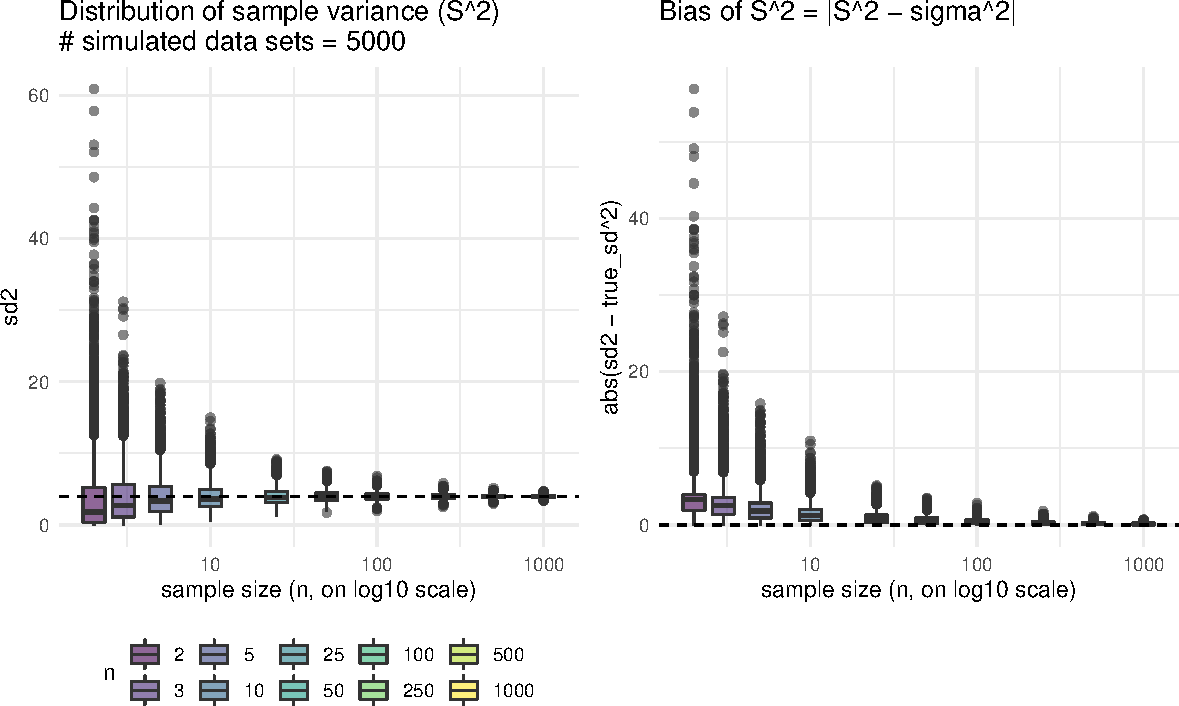
\includegraphics[width=1\linewidth]{class_notes_files/figure-latex/unnamed-chunk-9-1} \end{center}

\begin{Shaded}
\begin{Highlighting}[]
\CommentTok{# calculate variances of S^2}
\NormalTok{simdata_vars <-}\StringTok{ }\NormalTok{simdata }\OperatorTok\StringTok{ }\KeywordTok{group_by}\NormalTok{(nn) }\OperatorTok\StringTok{ }\KeywordTok{summarize}\NormalTok{(}\KeywordTok{var}\NormalTok{(sd2))}
\NormalTok{knitr}\OperatorTok{::}\KeywordTok{kable}\NormalTok{(simdata_vars, }\DataTypeTok{caption =} \StringTok{"Estimate of var(S_n^2) for various n"}\NormalTok{)}
\end{Highlighting}
\end{Shaded}

\begin{longtable}[]{@{}rr@{}}
\caption{Estimate of var(S\_n\^{}2) for various n}\tabularnewline
\toprule
nn & var(sd2)\tabularnewline
\midrule
\endfirsthead
\toprule
nn & var(sd2)\tabularnewline
\midrule
\endhead
2 & 33.4532308\tabularnewline
3 & 15.4419739\tabularnewline
5 & 8.0656179\tabularnewline
10 & 3.6600892\tabularnewline
25 & 1.3242583\tabularnewline
50 & 0.6578749\tabularnewline
100 & 0.3222768\tabularnewline
250 & 0.1288456\tabularnewline
500 & 0.0637904\tabularnewline
1000 & 0.0316714\tabularnewline
\bottomrule
\end{longtable}

We also know that continuous functions of a sequence of random variables
converge in probability if the sequence of random variables itself
converges in probability:

\noindent\textbf{Continuous mapping theorem: (Theorem 5.5.4 Convergence in probability of a function of a sequence of random variables)}
Suppose that \(Y_1, Y_2, \ldots\) converges in probability to a random
variable \(Y\) (or constant \(\theta\)) and that \(h\) is a continuous
function. Then \(h(Y_1), h(Y_2), \ldots\) converges in probability to
\(h(Y)\) (or \(h(\theta))\).

For example, since \(S^2 \to_p \sigma^2\) then
\(\sqrt{S^2} \to_p \sqrt{\sigma^2}\), or \(S \to_p \sigma\).

\hypertarget{convergence-in-distribution}{%
\subsection{Convergence in
distribution}\label{convergence-in-distribution}}

Convergence in distribution examines what happens to the distribution
function (specifically, the CDF) of a sequence of random variables as
\(n \to \infty\).

\noindent\textbf{Definition 5.5.10 Convergence in distribution} A
sequence of random variables \(Y_1, Y_2, \ldots,\) \emph{converges in
distribution} to a random variable \(Y\) if
\[\lim_{n\to\infty} F_{Y_n}(y) = F_Y(y)\] at all points \(y\) where
\(F_Y(y)\) is continuous.

\textbf{Example 5.5.11 Maximum of uniforms} If \(X_1, X_2, \ldots\) are
\(iid\) uniform(0,1), what happens to \(X_{(n)}\) as \(n\to\infty\)? We
can show \(X_{(n)}\to_p 1\): \begin{align*}
P(|X_{(n)} - 1| \geq \epsilon) &= P(X_{(n)} \leq 1 - \epsilon) + P(X_{(n)} \geq 1 + \epsilon)\\
&= P(X_{(n)} \leq 1 - \epsilon) + 0\\
&= \prod_{i=1}^n P(X_i \leq 1 - \epsilon)\\
&= [P(X_i \leq 1 - \epsilon)]^n = (1-\epsilon)^n \to 0
\end{align*} Now we can show \(Y_n = n(1-X_{(n)})\) converges in
distribution to \(Y \sim\) Exponential(1) random variable. In order to
show this, we need to show that the limit of the cdf of \(n(1-X_{(n)})\)
is the cdf of an Exponential(1) distribution.

In the above proof of convergence in probability, let
\(\epsilon = t/n\). Now,
\[P(X_{(n)} \leq 1 - \epsilon) =  P(X_{(n)} \leq 1 - t/n) = (1-t/n)^n \to e^{-t}\]
The limit is true by the definition of the exponential function. Upon
rearranging, we have
\[F_{Y_n}(t) = P(n(1-X_{(n)}) \leq t) = P(X_{(n)} \leq 1 - t/n) \to e^{-t} = F_y(t)\]
and hence \(Y_n \to_d Y\).

We can simulate this data and show convergence of the (approximate)
distribution of the simulated data. First let's show convergence in
probability of \(X_{(n)} \to_p 1\).

\begin{Shaded}
\begin{Highlighting}[]
\NormalTok{nsims <-}\StringTok{ }\DecValTok{5000}
\NormalTok{nn_all <-}\StringTok{ }\KeywordTok{c}\NormalTok{(}\DecValTok{2}\NormalTok{, }\DecValTok{3}\NormalTok{, }\DecValTok{5}\NormalTok{, }\DecValTok{10}\NormalTok{, }\DecValTok{25}\NormalTok{, }\DecValTok{50}\NormalTok{, }\DecValTok{100}\NormalTok{, }\DecValTok{250}\NormalTok{, }\DecValTok{500}\NormalTok{, }\DecValTok{1000}\NormalTok{)}

\KeywordTok{set.seed}\NormalTok{(}\DecValTok{100}\NormalTok{)}
\NormalTok{simdata <-}\StringTok{ }\NormalTok{nn_all }\OperatorTok\StringTok{ }
\StringTok{  }\NormalTok{purrr}\OperatorTok{::}\KeywordTok{map_df}\NormalTok{( }\OperatorTok{~}\KeywordTok{tibble}\NormalTok{(}\DataTypeTok{x =} \KeywordTok{runif}\NormalTok{(}\DataTypeTok{n=}\NormalTok{.}\OperatorTok{*}\NormalTok{nsims, }\DecValTok{0}\NormalTok{, }\DecValTok{1}\NormalTok{),}
                         \DataTypeTok{simrep =} \KeywordTok{rep}\NormalTok{(}\DecValTok{1}\OperatorTok{:}\NormalTok{nsims,}\DataTypeTok{each=}\NormalTok{.),}
                         \DataTypeTok{nn =}\NormalTok{ .) }\OperatorTok
\StringTok{  }\KeywordTok{group_by}\NormalTok{(nn,simrep) }\OperatorTok
\StringTok{    }\KeywordTok{summarize}\NormalTok{(}\DataTypeTok{xn =} \KeywordTok{max}\NormalTok{(x))}
\NormalTok{  ) }\OperatorTok\StringTok{ }\NormalTok{ungroup }\OperatorTok
\StringTok{  }\KeywordTok{mutate}\NormalTok{(}\DataTypeTok{yn =}\NormalTok{ nn}\OperatorTok{*}\NormalTok{(}\DecValTok{1}\OperatorTok{-}\NormalTok{xn))}

\NormalTok{p1 <-}\StringTok{ }\KeywordTok{ggplot}\NormalTok{(simdata, }\KeywordTok{aes}\NormalTok{(}\DataTypeTok{x=}\NormalTok{nn, }\DataTypeTok{y=}\NormalTok{xn, }\DataTypeTok{group=}\NormalTok{nn, }\DataTypeTok{fill=}\KeywordTok{factor}\NormalTok{(nn)))}\OperatorTok{+}
\StringTok{  }\KeywordTok{geom_boxplot}\NormalTok{(}\DataTypeTok{alpha=}\NormalTok{.}\DecValTok{6}\NormalTok{)}\OperatorTok{+}
\StringTok{  }\KeywordTok{scale_x_log10}\NormalTok{()}\OperatorTok{+}
\StringTok{  }\KeywordTok{xlab}\NormalTok{(}\StringTok{"sample size (n, on log10 scale)"}\NormalTok{)}\OperatorTok{+}
\StringTok{  }\KeywordTok{geom_hline}\NormalTok{(}\DataTypeTok{yintercept =}\DecValTok{1}\NormalTok{, }\DataTypeTok{lty=}\DecValTok{2}\NormalTok{)}\OperatorTok{+}
\StringTok{  }\KeywordTok{ggtitle}\NormalTok{(glue}\OperatorTok{::}\KeywordTok{glue}\NormalTok{(}\StringTok{"Distribution of X_(n)}\CharTok{\textbackslash{}n}\StringTok{# simulated data sets = \{nsims\}"}\NormalTok{))}\OperatorTok{+}
\StringTok{  }\KeywordTok{theme}\NormalTok{(}\DataTypeTok{legend.position=}\StringTok{"bottom"}\NormalTok{)}\OperatorTok{+}
\StringTok{  }\KeywordTok{scale_fill_viridis_d}\NormalTok{(}\DataTypeTok{name=}\StringTok{"n"}\NormalTok{)}

\NormalTok{p2 <-}\StringTok{ }\KeywordTok{ggplot}\NormalTok{(simdata, }\KeywordTok{aes}\NormalTok{(}\DataTypeTok{x=}\NormalTok{nn, }\DataTypeTok{y=}\KeywordTok{abs}\NormalTok{(xn}\DecValTok{-1}\NormalTok{), }\DataTypeTok{group=}\NormalTok{nn, }\DataTypeTok{fill=}\KeywordTok{factor}\NormalTok{(nn)))}\OperatorTok{+}
\StringTok{  }\KeywordTok{geom_boxplot}\NormalTok{(}\DataTypeTok{alpha=}\NormalTok{.}\DecValTok{6}\NormalTok{)}\OperatorTok{+}
\StringTok{  }\KeywordTok{scale_x_log10}\NormalTok{()}\OperatorTok{+}
\StringTok{  }\KeywordTok{xlab}\NormalTok{(}\StringTok{"sample size (n, on log10 scale)"}\NormalTok{)}\OperatorTok{+}
\StringTok{  }\KeywordTok{geom_hline}\NormalTok{(}\DataTypeTok{yintercept =}\DecValTok{0}\NormalTok{, }\DataTypeTok{lty=}\DecValTok{2}\NormalTok{)}\OperatorTok{+}
\StringTok{  }\KeywordTok{ggtitle}\NormalTok{(}\StringTok{"Bias of X_(n) = |X_(n) - 1|}\CharTok{\textbackslash{}n}\StringTok{ "}\NormalTok{)}\OperatorTok{+}
\StringTok{  }\KeywordTok{scale_fill_viridis_d}\NormalTok{(}\DataTypeTok{guide=}\OtherTok{FALSE}\NormalTok{)}

\NormalTok{p1 }\OperatorTok{+}\StringTok{ }\NormalTok{p2}
\end{Highlighting}
\end{Shaded}

\begin{center}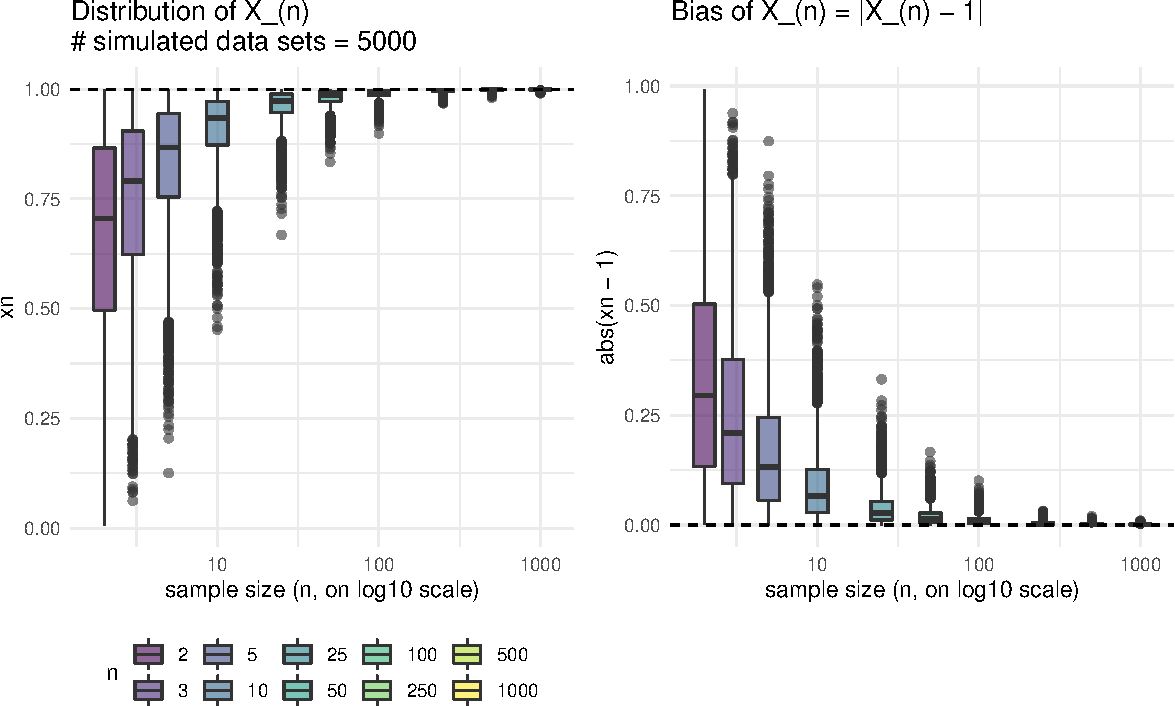
\includegraphics[width=1\linewidth]{class_notes_files/figure-latex/unnamed-chunk-10-1} \end{center}

\begin{Shaded}
\begin{Highlighting}[]
\CommentTok{# calculate variances of X_(n)}
\NormalTok{simdata_vars <-}\StringTok{ }\NormalTok{simdata }\OperatorTok\StringTok{ }\KeywordTok{group_by}\NormalTok{(nn) }\OperatorTok\StringTok{ }\KeywordTok{summarize}\NormalTok{(}\KeywordTok{var}\NormalTok{(xn))}
\NormalTok{knitr}\OperatorTok{::}\KeywordTok{kable}\NormalTok{(simdata_vars, }\DataTypeTok{caption =} \StringTok{"Estimate of var(X_(n)) for various n"}\NormalTok{)}
\end{Highlighting}
\end{Shaded}

\begin{longtable}[]{@{}rr@{}}
\caption{Estimate of var(X\_(n)) for various n}\tabularnewline
\toprule
nn & var(xn)\tabularnewline
\midrule
\endfirsthead
\toprule
nn & var(xn)\tabularnewline
\midrule
\endhead
2 & 0.0549248\tabularnewline
3 & 0.0376370\tabularnewline
5 & 0.0198240\tabularnewline
10 & 0.0067927\tabularnewline
25 & 0.0013699\tabularnewline
50 & 0.0003746\tabularnewline
100 & 0.0000989\tabularnewline
250 & 0.0000171\tabularnewline
500 & 0.0000040\tabularnewline
1000 & 0.0000010\tabularnewline
\bottomrule
\end{longtable}

Now, we show convergence in distribution of \(Y_n = n(1-X_{(n)})\). Note
first that \(Y_n\) does not appear to converge in probability to a
constant since the variance does not get smaller as \(n\to\infty\) (left
panel). {[}Note the median looks like it is stabilizing, and in fact it
is converging to the median of Exp(1) which is ln(2) = 0.693\ldots{}{]}.
However, if we look at the approximate distribution of \(Y_n\) compared
to an Exp(1) distribution, we can see convergence of the CDFs to the CDF
of Exp(1) represented by the dashed line (right panel).

\begin{Shaded}
\begin{Highlighting}[]
\NormalTok{p1 <-}\StringTok{ }\KeywordTok{ggplot}\NormalTok{(simdata, }\KeywordTok{aes}\NormalTok{(}\DataTypeTok{x=}\NormalTok{nn, }\DataTypeTok{y=}\NormalTok{yn, }\DataTypeTok{group=}\NormalTok{nn, }\DataTypeTok{fill=}\KeywordTok{factor}\NormalTok{(nn)))}\OperatorTok{+}
\StringTok{  }\KeywordTok{geom_boxplot}\NormalTok{(}\DataTypeTok{alpha=}\NormalTok{.}\DecValTok{6}\NormalTok{)}\OperatorTok{+}
\StringTok{  }\KeywordTok{scale_x_log10}\NormalTok{()}\OperatorTok{+}
\StringTok{  }\KeywordTok{xlab}\NormalTok{(}\StringTok{"sample size (n, on log10 scale)"}\NormalTok{)}\OperatorTok{+}
\StringTok{  }\KeywordTok{ggtitle}\NormalTok{(glue}\OperatorTok{::}\KeywordTok{glue}\NormalTok{(}\StringTok{"Distribution of Y_n = n*(1-X_(n))}\CharTok{\textbackslash{}n}\StringTok{# simulated data sets = \{nsims\}"}\NormalTok{))}\OperatorTok{+}
\StringTok{  }\KeywordTok{theme}\NormalTok{(}\DataTypeTok{legend.position=}\StringTok{"bottom"}\NormalTok{)}\OperatorTok{+}
\StringTok{  }\KeywordTok{scale_fill_viridis_d}\NormalTok{(}\DataTypeTok{name=}\StringTok{"n"}\NormalTok{)}

\NormalTok{p2 <-}\StringTok{ }\KeywordTok{ggplot}\NormalTok{(simdata, }\KeywordTok{aes}\NormalTok{(}\DataTypeTok{x=}\NormalTok{yn, }\DataTypeTok{group=}\NormalTok{nn, }\DataTypeTok{color=}\KeywordTok{factor}\NormalTok{(nn)))}\OperatorTok{+}
\StringTok{  }\KeywordTok{stat_ecdf}\NormalTok{()}\OperatorTok{+}
\StringTok{  }\KeywordTok{ggtitle}\NormalTok{(}\StringTok{"Empirical CDF of simulated data Y_n"}\NormalTok{)}\OperatorTok{+}
\StringTok{  }\KeywordTok{ylab}\NormalTok{(}\StringTok{"eCDF and CDF"}\NormalTok{)}\OperatorTok{+}
\StringTok{  }\KeywordTok{stat_function}\NormalTok{(}\DataTypeTok{fun=}\NormalTok{pexp, }\DataTypeTok{color=}\StringTok{"black"}\NormalTok{, }\DataTypeTok{lty=}\DecValTok{2}\NormalTok{)}\OperatorTok{+}
\StringTok{  }\KeywordTok{scale_color_viridis_d}\NormalTok{(}\DataTypeTok{guide=}\OtherTok{FALSE}\NormalTok{)}

\NormalTok{p1}\OperatorTok{+}\NormalTok{p2}
\end{Highlighting}
\end{Shaded}

\begin{center}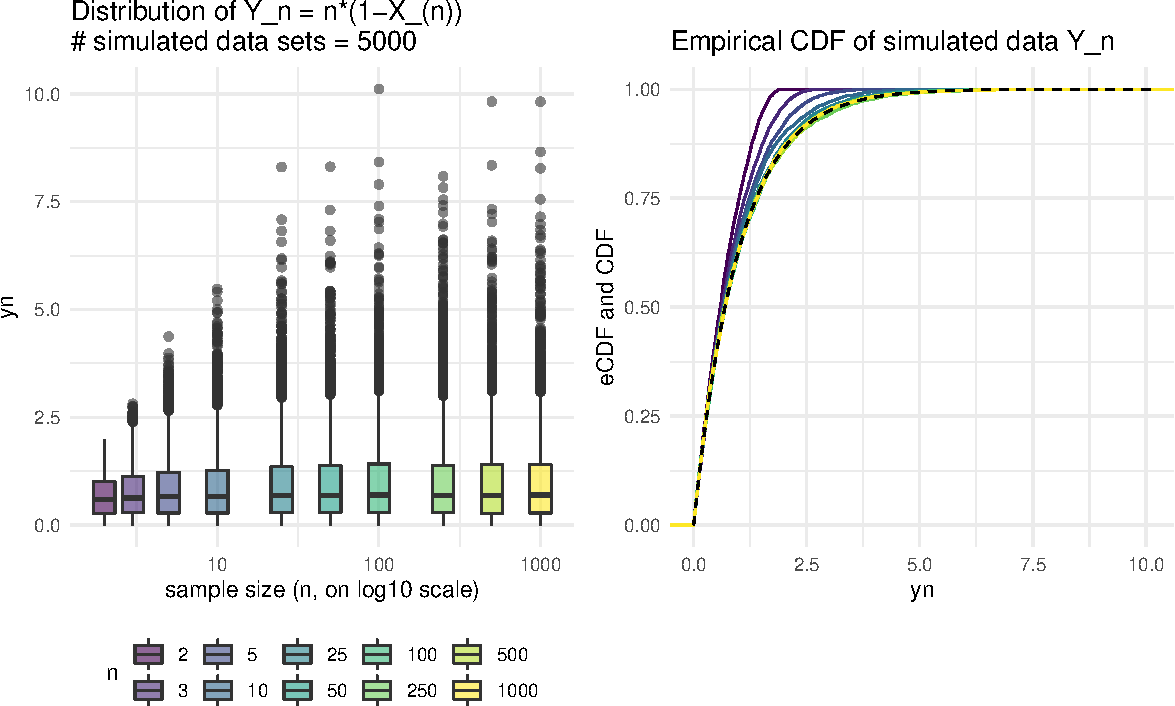
\includegraphics[width=1\linewidth]{class_notes_files/figure-latex/unnamed-chunk-11-1} \end{center}

\hypertarget{important-theorems-about-convergence-in-distribution}{%
\subsubsection{Important theorems about convergence in
distribution}\label{important-theorems-about-convergence-in-distribution}}

\emph{Convergence in probability is ``stronger'' than convergence in
distribution since \(\to_p\) implies \(\to_d\).}

\textbf{Theorem 5.5.12 Convergence in probability implies converge in
distribution:} If the sequence of random variables,
\(Y_1, Y_2, \ldots,\) converges in probability to a random variable
\(Y\), the sequence also converges in distribution to \(Y\).

\emph{Convergence in distribution to a constant has a special property
that it is equivalent to convergence in probability}.

\textbf{Theorem 5.5.13 Convergence in distribution to constant =
convergence in probability to constant:} The sequence of random
variables \(Y_1, Y_2, \ldots,\) converges in probability to a constant
\(\mu\) if and only if the sequence also converges in distribution to
\(\mu.\) That is, the statement
\[P(| Y_n - \mu| > \delta) \to 0 \mbox{ for every } \delta > 0\] is
equivalent to \[P(Y_n \leq y) \to \begin{cases}
0, & \mbox{if } y< \mu\\
1, & \mbox{if } y> \mu.
\end{cases}
\]

\emph{An important and famous example of convergence in distribution is
the convergence of the distribution of the sample mean, called the
Central Limit Theorem. One version of the CLT is as follows:}

\noindent\textbf{Central Limit Theorem (Theorem 5.5.14)} Let
\(X_1, X_2, \ldots\) be a sequence of \(iid\) random variables whose
moment generating functions (mgfs) exist in a neighborhood of 0 (that
is, \(M_{X_i}(t)\) exists for \(|t| < h\), for some positive \(h\)). Let
\(E(X_i) =\mu\) and \(Var(X_i) = \sigma^2 > 0\). (Both \(\mu\) and
\(\sigma^2\) are finite since the mgf exists.) Define
\(\Xbar_n = (1/n) \sumin X_i\). Let \(G_n(x)\) denote the cdf of
\(\sqrt{n} (\Xbar_n - \mu)/\sigma\). Then, for any
\(x, -\infty < x < \infty\),
\[\lim_{n\to\infty} G_n(x) = \int_{-\infty}^{x} \frac{1}{\sqrt{2\pi}} e^{-y^2/2} dy;\]
that is, \(\sqrt{n}(\Xbar_n - \mu)/\sigma\) has a limiting standard
normal distribution:
\[\frac{\sqrt{n}(\Xbar_n - \mu)}{\sigma} \to_d \Nsc(0,1)\]

See the proof in C\&B (uses Taylor series expansion of the moment
generating function).

\emph{A very useful theorem for proving convergence in distribution when
you have a sum or product of random variables is Slutsky's Theorem:}

\textbf{Slutsky's Theorem (Theorem 5.5.17)}: If
\(X_n \xrightarrow{d} X\) in distribution and \(Y_n \xrightarrow{p} a\),
with \(a\) constant, in probability, then:

\begin{itemize}
\item[a.] $Y_n X_n \xrightarrow{d}  aX$ (in distribution)
\item[b.] $X_n + Y_n \xrightarrow{d}  X + a$ (in distribution)
\end{itemize}

\begin{itemize}
\tightlist
\item
  Note that \(Y_n\) must converge in probability to a constant, not a
  random variable. Otherwise, these relationships do not always hold.
\item
  Also, if \(X_n \to_p X\) in probability, the above theorem still holds
  since this implies that \(X_n \to_d X\) in distribution.
\end{itemize}

\noindent\textbf{Example 5.5.18 Normal approximation with estimated variance}:
Suppose that
\[\frac{\sqrt{n} (\Xbar_n - \mu) }{\sigma} \to_d \Nsc(0,1)\] but the
value of \(\sigma\) is unknown. We have seen in Example 5.5.3 that, if
\(\lim_{n\to\infty} \Var S_n^2 = 0\), then \(S_n^2 \to \sigma^2\) in
probability. We can show (Exercise 5.32) that \(\sigma/S_n \to 1\) in
probability. Therefore, by Slutsky's Theorem
\[\frac{\sqrt{n} (\Xbar_n - \mu) }{S_n} = \frac{\sigma}{S_n}\frac{\sqrt{n} (\Xbar_n - \mu) }{\sigma} \to_d \Nsc(0,1).\]

\emph{Another very useful theorem about convergence in distribution is
the Delta Method. It is used when we need to determine the asymptotic
distribution of a function of a statistic. You can think of this as ``a
generalized CLT'' since it can be used to show convergence of a function
of} \(\Xbar\).

\textbf{Delta Method (Theorem 5.5.24)} Let \(Y_n\) be a sequence of
random variables that satisfies
\[\sqrt{n}(Y_n - \theta) \xrightarrow{d} \Nsc(0,\sigma^2).\] For a given
function \(g\) and a specific value of \(\theta\), assuming
\(g^\prime(\theta)\) exists and is not 0, then:
\[\sqrt{n}\left[g(Y_n) - g(\theta)\right] \xrightarrow{d} \Nsc(0, \sigma^2[g^\prime(\theta)]^2).\]

\noindent\textbf{Proof:} The Taylor expansion of \(g(Y_n)\) around
\(Y_n = \theta\) is
\[g(Y_n) = g(\theta) + g^\prime(\theta) (Y_n - \theta) + \mbox{Remainder}\]
where the remainder \(\to 0\) as \(Y_n \to \theta\). Since
\(Y_n \to \theta\) in probability it follows that the remainder (call it
\(Z_n\)) \(\to 0\) in probability. So, by applying Slutsky's Theorem
\[\sqrt{n}[g(Y_n) - g(\theta)] = g^\prime(\theta) \sqrt{n} (Y_n - \theta) + Z_n \to_d g^\prime(\theta)\Nsc(0, \sigma^2) + 0 = \Nsc(0,\sigma^2[g^\prime(\theta)]^2)\]
and the result follows.

\noindent\textbf{Example 5.5.25:} Suppose \(X_i\) is a random variable
with \(E_\mu X_i = \mu \neq 0\). Suppose we want to find the
distribution of \(\frac{1}{\Xbar}\). By the Delta Method we have
\(g^\prime(\mu) = - \mu^{-2}\) and
\[\sqrt{n}\left(\frac{1}{\Xbar} - \frac{1}{\mu} \right) \to \Nsc\left(0, \left( \frac{1}{\mu}\right)^4 \Var_\mu X\right)\]

However, we may not know the variance of \(X\), so we need to estimate
it with \(S^2\). Also, we need to estimate \(\mu\) with \(\Xbar\). We
can estimate the whole variance:
\[\widehat{\Var} \left( \frac{1}{\Xbar} \right) \approx \left(\frac{1}{\Xbar}\right)^4 S^2.\]
Since both \(\Xbar\) and \(S^2\) are consistent estimators of \(\mu\)
and \(\sigma^2\), we can apply Slutsky's Theorem to conclude that for
\(\mu \neq 0\),
\[\frac{\sqrt{n} \left( \frac{1}{\Xbar} - \frac{1} {\mu} \right)}{\left( \frac{1}{\Xbar} \right)^2 S} \to_d \Nsc(0,1)\]
in distribution.

\emph{Sometimes the derivative of \(g\) is 0 at \(\theta\) so we must
use the second-order Delta Method:}

\textbf{Second-order Delta Method (Theorem 5.5.26)} Let \(Y_n\) be a
sequence of random variables that satisfies
\[\sqrt{n}(Y_n - \theta) \xrightarrow{d} \Nsc(0,\sigma^2).\] For a given
function \(g\) and a specific value of \(\theta\), suppose that
\(g^\prime(\theta) = 0\) and \(g^{\prime\prime}(\theta)\) exists and is
not 0. Then
\[n[g(Y_n) - g(\theta)] \to \sigma^2\frac{g^{\prime\prime}(\theta)}{2}\chi^2_1\]
That is, the asymptotic distribution is a chi-square random variable.
{[}This is also proven using Taylor Series expansions but out to the
second degree polynomial, and Slutsky's theorem.{]}

\newpage

\hypertarget{asymptotic-evaluations-chapter-10-with-some-review-of-chapters-5-and-7}{%
\section{Asymptotic Evaluations (Chapter 10, with some review of
Chapters 5 and
7)}\label{asymptotic-evaluations-chapter-10-with-some-review-of-chapters-5-and-7}}

\begin{itemize}
\tightlist
\item
  So far we have considered \emph{finite-sample criteria} for inference
  about a parameter \(\theta\). That is, the distributions of test
  statistics were valid for finite sample sizes.
\item
  Asymptotics are concerned with the properties of estimators, random
  variables, and hypothesis tests as the sample size(s) increases.
\item
  ``asymptotics uncover the most fundamental properties of a procedure
  and give us a very powerful and general evaluation tool''--C\&B
\item
  We are concerned with a sequence of estimators
  \(W_n = W_n(X_1,\ldots,X_n)\). Often \(W_n = \thetahat_n\) the MLE of
  \(\theta\).
\end{itemize}

\hypertarget{consistency-sim-relates-to-the-expectation-of-an-estimator}{%
\subsection{\texorpdfstring{Consistency \(\sim\) relates to the
expectation of an
estimator}{Consistency \textbackslash{}sim relates to the expectation of an estimator}}\label{consistency-sim-relates-to-the-expectation-of-an-estimator}}

\begin{itemize}
\item As $n\to\infty$, an estimator should converge to the ``correct" value = the parameter of interest.
\item Equivalently, bias should go to 0; we want our estimator to be "asymptotically unbiased".
\item We would not want an inconsistent estimator, since then we are tending towards bias no matter how large of a sample (even the entire population) we obtain.
\end{itemize}

\textbf{Definition 10.1.1 Consistency (convergence in probability to a
constant)} A sequence of estimators \(W_n = W_n(\Xndots)\) is a
\emph{consistent sequence of estimators} of the parameter \(\theta\) if,
\(W_n \xrightarrow{p} \theta\).

\begin{itemize}
\tightlist
\item
  Previously we saw that \(\Xbar_n \xrightarrow{p} \mu = E(X_i)\) by the
  WLLN and \(S^2_n \xrightarrow{p} \sigma^2 = Var(X_i)\) so these are
  examples of consistent estimators.
\end{itemize}

\hypertarget{mean-square-error-to-0-implies-consistency}{%
\subsubsection{\texorpdfstring{Mean Square Error \(\to 0\) implies
consistency}{Mean Square Error \textbackslash{}to 0 implies consistency}}\label{mean-square-error-to-0-implies-consistency}}

In order to prove consistency, we can also examine the behavior of the
finite sample variance and bias of our estimator. Together, this is the
mean square error.

\begin{itemize}
\item For an estimator $\thetahat$ of $\theta$ we wish to  performance or `goodness' of the estimator.
\item Hence we estimate the deviation from $\thetahat$ to the true value.
\item The {\em absolute error} $|\thetahat - \theta|$ measures this.
\item However, the square of this $(\thetahat - \theta)^2$ also measures this deviation but has nicer mathematical properties
\end{itemize}

\noindent\textbf{Definition} The \emph{mean square error (MSE)} of an
estimator \(W_n\) of the parameter \(\theta\) is the function
\(E(W_n - \theta)^2\). We can denote this as \(MSE_\theta({W_n}).\) This
is also called the quadratic loss function.

An important mathematical property of MSE is (from 7.3.1):
\[MSE_\theta(W_n) = E_\theta[ (W_n - \theta)^2] = E_\theta[(W_n - E_\theta(W_n))^2] + [E_\theta(W_n) - \theta]^2= Var_\theta W_n + [Bias_\theta W_n]^2\]

\begin{itemize}
\item The MSE has two components: the variability of an estimator (precision) and the bias (accuracy)
\item We need to find estimators that control both variance and bias.
\item For an unbiased estimator we only need to control variance since then $MSE_\thetahat = Var(\thetahat)$
\end{itemize}

In general when estimating a parameter \(\theta\) via \(W_n\), if
\(Var_\theta(W_n) \to 0\) and \(Bias_\theta(W_n) \to 0\) as
\(n\to \infty\), then the estimator is consistent for \(\theta\). This
can be seen since by using Chebychev's Inequality (Theorem 3.6.1) to
link the definition of convergence in probability to the MSE:

\[P_\theta(|W_n - \theta| \geq \delta) \leq \frac{E_\theta[(W_n - \theta)^2]}{\delta^4}\]
so if, for every \(\theta \in \Theta,\)
\[\lim_{n\to\infty} E_\theta [(W_n - \theta)^2] =\lim_{n\to\infty} MSE_\theta(W_n) = 0,\]
then the sequence of estimators is consistent for \(\theta\).
Furthermore, by (7.3.1),
\[MSE_\theta(W_n) = E_\theta[ (W_n - \theta)^2] = Var_\theta W_n + [Bias_\theta W_n]^2\]
Combining these facts, we have the following theorem:

\noindent\textbf{Theorem 10.1.3} If \(W_n\) is a sequence of estimators
of a parameter \(\theta\) satisfying

\begin{enumerate}
\item $\lim_{n\to\infty} Var_\theta W_n = 0,$
\item $\lim_{n\to\infty} Bias_\theta W_n = 0,$
\end{enumerate}

for every \(\theta \in \Theta\), then \(W_n\) is a consistent sequence
of estimators of \(\theta\).

In other words, if \(MSE_\theta(W_n) \to 0\), then \(W_n\) is consistent
for \(\theta\).

\textbf{Example general variance} Let \(X_1, X_2, \ldots X_n\) be iid
\(\Nsc(\mu,\sigma^2)\) with known \(\sigma < \infty\). Then
\(W_n = \Xbar_n\) is an estimator of \(\mu\).

\begin{enumerate}
\item $\lim_{n\to\infty} Var_\theta \Xbar = \lim_{n\to\infty} \frac{\sigma^2}{n} = 0,$
\item $\lim_{n\to\infty} Bias_\theta \Xbar = \lim_{n\to\infty} E(\Xbar) - \mu = \mu - \mu = 0,$
\end{enumerate}

So by Thm 10.1.3, \(\Xbar_n\) is a consistent estimator of \(\mu\).

\hypertarget{linear-combinations-of-consistent-estimators}{%
\subsubsection{Linear combinations of consistent
estimators}\label{linear-combinations-of-consistent-estimators}}

We can also construct consistent estimators from other consistent
estimators:

\noindent\textbf{Theorem 10.1.5} Let \(W_n\) be a consistent sequence of
estimators of a parameter \(\theta\). Let \(a_1, a_2, \ldots\) and
\(b_1, b_2,\ldots\) be sequences of constants satisfying

\begin{enumerate}
\item $\lim_{n\to\infty} a_n = 1$,
\item $\lim_{n\to\infty} b_n = 0$.
\end{enumerate}

Then the sequence \(U_n = a_n W_n + b_n\) is a consistent sequence of
estimators of \(\theta\).

\noindent\textbf{Proof:} Use Slutsky's theorem from chapter 5.

\noindent\textbf{Example: Consistency of Normal variance estimates} Let
\(\Xndots\) be iid \(\Nsc(\mu,\sigma^2)\). Let
\(S^2 = \frac{1}{n-1} \sumin (X_i - \Xbar)^2\). We have seen that
\(E_{\mu,\sigma^2}(S^2) = \sigma^2\) and
\(Var_{\mu,\sigma^2}(S^2) = 2\frac{\sigma^4}{n-1}\). So, \(S^2\) is a
consistent estimator of \(\sigma^2\).

Since
\(\sigmahat^2 = \frac{1}{n} \sumin(X_i - \Xbar)^2 = \frac{n}{n-1}S^2,\)
\(\sigmahat^2\) is also a consistent estimator of \(\sigma^2\).

We could have also proven this by showing that \(\sigmahat^2\) is
asymptotically unbiased (even though it has bias in finite samples, the
bias goes to 0 as \(n \to \infty\)) and that the variance of
\(\sigmahat^2\) goes to 0.

\hypertarget{consistency-of-mles}{%
\subsubsection{Consistency of MLEs}\label{consistency-of-mles}}

A very important result!

\noindent\textbf{Theorem 10.1.6 Consistency of MLEs} Let
\(X_1, X_2, \ldots\) be iid \(f(x|\theta)\), and let
\(L(\theta|\bx) = \prod_{i=1}^n f(x_i |\theta)\) be the likelihood
function. Let \(\thetahat\) denote the MLE of \(\theta\). Let
\(\tau(\theta)\) be a continuous function of \(\theta\). Under certain
regularity conditions on \(f(x|\theta)\) and, hence, \(L(\theta|\bx)\),
for every \(\delta >0\) and every \(\theta \in \Theta\),
\[\lim_{n\to\infty} P_\theta(|\tau(\thetahat) - \tau(\theta)| \geq \delta) = 0.\]
That is, \(\tau (\thetahat)\) is a consistent estimator of
\(\tau(\theta)\).

\noindent\textbf{Proof sketch:} Show that
\(\frac{1}{n} \log \Lsc(\thetahat | \bx)\) converges almost surely (a
stronger convergence than convergence in probability) to
\(E_\theta(\log f(X|\theta))\) for every \(\theta \in \Theta\). This
(under some conditions) implies that
\(\thetahat \xrightarrow{p} \theta\) and, hence
\(\tau(\thetahat) \xrightarrow{p} \tau(\theta)\).

For regularity conditions (related to identifiability, differentiable
\(f\), etc) see Miscellanea 10.6.2.

\begin{itemize}
\item There are extensions to non-iid settings, for example regression.
\item So, under regularity conditions, MLE's get closer and closer to the parameters they are estimating as the sample size gets large.
\end{itemize}

\hypertarget{efficiency-sim-relates-to-the-variance-of-the-estimator}{%
\subsection{\texorpdfstring{Efficiency \(\sim\) relates to the variance
of the
estimator}{Efficiency \textbackslash{}sim relates to the variance of the estimator}}\label{efficiency-sim-relates-to-the-variance-of-the-estimator}}

\begin{itemize}
\item Consistency is concerned with asymptotic accuracy. We should also be concerned with the asymptotic variance of an estimator.
\item We'd also like the MLE estimator to have small variance for large samples and to have a limiting distribution that we can use for obtaining tests and confidence intervals.
\item In many cases for an estimator $W_n$, Var$(W_n) \to 0$ as $n\to \infty$ since it is a consistent estimator. So we need to evaluate the variance of $k_n W_n$ where $k_n$ is some normalizing constant to force the variance to a limit that is not 0.
\end{itemize}

\hypertarget{efficient-estimator-finite-sample-property}{%
\subsubsection{Efficient Estimator (finite sample
property)}\label{efficient-estimator-finite-sample-property}}

Recall \textbf{Fisher's Information} and the three equivalent
definitions:
\[I(\theta) = I_1(\theta) = E_\theta\left[\left(\frac{\partial}{\partial\theta} \log f_X(x|\theta)\right)^2\right] =
Var_\theta\left[\frac{\partial}{\partial\theta}  \log f_X(x|\theta)\right] = 
 - E_\theta\left[\frac{\partial^2}{\partial \theta^2} \log f_X(x|\theta)\right]\]

We use the notation \(I_n(\theta)\) to denote the information number
(expected information) based on a sample of \(n\) observations.
\[I_n(\theta) = - E_\theta\left[\frac{\partial^2}{\partial \theta^2} \sumin \log f_X(x_i|\theta)\right]
=
- \sumin E_\theta\left[\frac{\partial^2}{\partial \theta^2}\log f_X(x_i|\theta)\right] = nI_1(\theta)\]

We use Fisher's Information to bound the variance of an estimator with
Cramer-Rao's Inequality (a.k.a the information inequality):
\[Var(\thetahat) \geq \frac{[\frac{\partial}{\partial\theta} E_\theta(\thetahat)]^2}{n I_1(\theta)}\]
As the information number increases, we can bound the variance with a
smaller number.

\noindent\textbf{Definition:} When the equality holds, that is,
\(Var(\thetahat) = \frac{[\frac{\partial}{\partial\theta} E_\theta(\thetahat)]^2}{n I(\theta)}\),
the estimator \(\thetahat\) is said to be an \emph{efficient estimator}
of its expectation \(E_\theta(\thetahat)\). If
\(E_\theta(\thetahat) = \theta\) then \(\thetahat\) is an efficient
estimator of \(\theta\). If an estimator is unbiased and its variance
reaches the CR lower bound, then it is the minimum variance unbiased
estimator (MVUE).

\hypertarget{asymptotic-variance}{%
\subsubsection{Asymptotic variance}\label{asymptotic-variance}}

\begin{itemize}
\item In many cases for an estimator $W_n$, Var$(W_n) \to 0$ as $n\to \infty$ since it is a consistent estimator. So we need to evaluate the variance of $k_n W_n$ where $k_n$ is some normalizing constant (function of $n$) to force the variance to a limit that is not 0.
\item In particular, we want to choose $\{ k_n\}$ such that we have an asymptotically normal distribution with a particular asymptotic variance.
\item Then we can compare variances of the asymptotic distributions for different estimators to see which is smallest.
\end{itemize}

\noindent\textbf{Definition 10.1.9} For an estimator \(W_n\), suppose
that \(k_n (W_n - \tau(\theta)) \xrightarrow{d} \Nsc(0,\sigma^2)\)) in
distribution. That is, \[
\lim_{n\to\infty} \mbox{cdf of } k_n (W_n - \tau(\theta)) = \mbox{ cdf of } \Nsc(0,\sigma^2).\]
The parameter \(\sigma^2\) is called the \emph{asymptotic variance} of
\(W_n\).

\begin{itemize}
\item If two estimators have the same asymptotic distribution and the same asymptotic mean but different asymptotic variances, we prefer the estimator with the smaller variance.
\end{itemize}

\noindent\textbf{Definition 10.1.11} Let \(W_n\) be a sequence of
estimators based on \(\Xndots \sim_{iid} f(x|\theta)\). \(W_n\) is
\emph{asymptotically efficient} for a parameter \(\tau(\theta)\) if
\(\sqrt{n} (W_n - \tau(\theta)) \to \Nsc(0, v[\tau(\theta)])\) in
distribution where \(v[\tau(\theta)] >0\) and
\[v[\tau(\theta)] = \frac{[\tau^\prime(\theta)]^2}{E_\theta((\frac{\partial}{\partial\theta} \log f(X|\theta))^2)} = \frac{[\tau^\prime(\theta)]^2}{I_1(\theta)}.\]
That is, the asymptotic variance of \(W_n\) achieves the Cramer-Rao
Lower Bound for unbiased estimators of \(\tau(\theta)\).

When \(\tau(\theta) = \theta\), then \(\tau^\prime(\theta) = 1\) so
\[v[\theta] = \frac{1}{I_1(\theta)}.\]

\begin{itemize}
\item Note, because we are multiplying by $\sqrt{n}$ we don't need the $n$ in the CRLB-- we use the density for a {\em single observation} in the $iid$ case. That is why the quantity in the denominator is based on the pdf (pmf) of a single observation.
\item Theorem 10.1.6 stated that MLEs are consistent (under general conditions). Under somewhat stronger regularity conditions, we have similar result for asymptotic efficiency.
\end{itemize}

\noindent\textbf{Theorem 10.1.12 Asymptotic efficiency of MLEs}: Let
\(X_1, X_2, \ldots\) be \(\sim_{iid} f(x|\theta)\), let \(\thetahat\)
denote the MLE of \(\theta\), and let \(\tau(\theta)\) be a continuous
function of \(\theta\). Under the regularity conditions in Misc. 10.6.2
on \(f(x|\theta)\) and hence,
\(\Lsc(\theta|\bx) = \prod_{i=1}^n f(x_i|\theta)\),
\[\sqrt{n} [\tau(\thetahat) - \tau(\theta)] \xrightarrow{d} \Nsc[0,v[\tau(\theta)]\]
where \(v[\tau(\theta)]\) is the Cramer-Rao Lower Bound. That is,
\(\tau(\thetahat)\) is a consistent and asymptotically efficient
estimator of \(\tau(\theta)\). (!)

So, the asymptotic variance of the MLE achieves the smallest possible
variance among unbiased estimators of \(\tau(\theta)\).

\noindent\textbf{Proof:} We first outline the proof showing the case
that \(\tau(\theta) = \theta\) to show that \(\thetahat\) is
asymptotically efficient.

Let \(\ell(\theta|\bx) = \sumin \log f(\bx_i |\theta)\) denote the
log-likelihood function and denote its derivatives by
\(\ell^\prime, \ell^{\prime\prime}, \ldots\). Obtain a Taylor's
expansion of the first derivative about the true value \(\theta_0\):
\[\ell^\prime(\theta|\bx) = \ell^\prime(\theta_0 | \bx) + (\theta - \theta_0) \ell^{\prime\prime}(\theta_0 |\bx) + Remainder\]
where \(Remainder\) represents the remaining terms that converge to 0
(specifically, they have the property \(Remainder/n \to 0\) as
\(n\to \infty\) under the regularity conditions).

Substitute \(\thetahat\) for \(\theta\):
\[\ell^\prime(\thetahat|\bx) = \ell^\prime(\theta_0 | \bx) + (\thetahat - \theta_0) \ell^{\prime\prime}(\theta_0 |\bx) + Remainder\]
The left-hand side \(\ell^\prime(\thetahat|\bx)\) is equal to 0 since
\(\thetahat\) is an MLE and we find the MLE by setting the derivative of
the log-likelihood to 0. Rearranging we have: \begin{align*}
(\thetahat - \theta_0) &= -\frac{\ell^\prime(\theta_0 | \bx)}{\ell(\theta_0 | \bx) + Remainder} \Leftrightarrow\\
\sqrt{n} (\thetahat - \theta_0)&= -\sqrt{n} \frac{\ell^\prime(\theta_0 | \bx)}{\ell^{\prime\prime}(\theta_0 | \bx)+Remainder}\\
&= - \frac{\ell^\prime(\theta_0 | \bx)/\sqrt{n}}{\ell^{\prime\prime}(\theta_0 | \bx)/n + Remainder/n}
\end{align*}

Since the remainder term \(Remainder/n \xrightarrow{p} 0\), to find the
asymptotic distribution of \(\sqrt{n}(\thetahat - \theta_0)\) we need to
find the asymptotic distribution of
\[\frac{\ell^\prime(\theta_0 | \bx)/\sqrt{n}}{-\ell^{\prime\prime}(\theta_0 | \bx)/n}\]

Let \(I_1(\theta_0) = 1/v(\theta)\) denote the information number for
one observation.

\emph{First consider the numerator}:

Now, since \(\Xndots\) are \(iid\) and
\(E(\ell^\prime(\theta_0|x_i)) = 0\), by the Central Limit Theorem:
\[\frac{\ell^\prime(\theta_0 | \bx)}{\sqrt{n}} = \sqrt{n} \left[\frac{1}{n} \sumin \ell^\prime(\theta_0|x_i)\right] \xrightarrow{d} \Nsc(0, Var_{\theta_0}[\ell^\prime(\theta_0|x_i)])\]
where
\[Var_{\theta_0}[\ell^\prime(\theta_0|x_i)] = E_{\theta_0} [-\ell^{\prime\prime}(\theta_0 |x_i)] = I_1(\theta_0) = 1/v(\theta) \mbox{ (definition of Fisher's Information)}\]

\emph{Now consider the denominator}:

Also, by the Weak Law of Large Numbers:
\[-\frac{1}{n} \ell^{\prime\prime}(\theta_0 |\bX) = -\frac{1}{n}\sumin \ell^{\prime\prime}(\theta_0 |x_i) \xrightarrow{p} I_1(\theta_0).\]

\emph{Num/Denom}:

So, by Slutsky's Theorem:
\[\sqrt{n} (\thetahat - \theta_0) =\left[-\frac{1}{n} \ell^{\prime\prime}(\theta_0 |\bX) \right]^{-1} \left[\frac{\ell^\prime(\theta_0 | \bx)}{\sqrt{n}} \right] \xrightarrow{d}
 \left[I_1(\theta_0)\right]^{-1} \Nsc(0,I_1(\theta_0)) =  \Nsc(0,1/I_1(\theta_0)) = \Nsc(0,v(\theta))\]

To extend to a general \(\tau(\theta)\), the Delta Method says that\\
\[\sqrt{n}(\tau(\theta) - \tau(\theta)) \xrightarrow{d} \Nsc(0, v(\theta)[\tau^\prime(\theta)]^2)\]
and in fact
\(v(\theta)[\tau^\prime(\theta)]^2 = [\tau^\prime(\theta)]^2/I(\theta_0)\)
is the CR lower bound for \(\tau(\theta)\).

\begin{itemize}
 \item Note on regularity conditions: For $iid$ samples from one parameter {\em regular} exponential families (parameter space contains an open interval), the MLE (obtained as a solution to likelihood equations) is asymptotically efficient. For multiparameter exponential families the results also hold provided the likelihood equations for the MLE have a solution.
 \end{itemize}

\noindent\textbf{Example 10.1.13 Asymptotic normality and consistency}
The above theorem shows that typically MLEs are efficient and
consistent. However, this is somewhat redundant, as efficiency is
defined only when the estimator is asymptotically normal and, as we will
illustrate, \emph{asymptotic normality implies consistency.}

Suppose that \[\sqrt{n}(W_n - \theta) \xrightarrow{d} \Nsc(0,\sigma^2)\]
then
\[\sqrt{n}\frac{W_n - \theta}{\sigma} \xrightarrow{d} \frac{1}{\sigma}\Nsc(0,\sigma^2) = \Nsc(0,1)\]
From Slutksy's Theorem:
\[W_n - \mu = \frac{\sigma}{\sqrt{n}} \left( \sqrt{n}\frac{W_n - \theta}{\sigma} \right) \to \lim_{n\to\infty}  \frac{\sigma}{\sqrt{n}}\Nsc(0,1) = 0.\]
so \(W_n - \mu \xrightarrow{d} 0\) which implies convergence in
probability to 0 (Thm 5.5.13 above). Hence, \(W_n\) is a consistent
estimator of \(\mu\).

\noindent\textbf{Example Normal MLE} Let
\(\Xndots \sim_{iid} \Nsc(\mu,\sigma^2), \sigma^2\) known. Then the MLE
of \(\mu\) is \(\Xbar\) and
\(\sqrt{n} (\Xbar - \mu) \sim \Nsc(0,\sigma^2)\). This is the exact
distribution. In this case, this is also the asymptotic distribution.
This result follows from the CLT but also the above theorem since
\begin{align*}
I_1(\mu) &=
E_\mu\left(- \frac{\partial^2}{\partial \mu^2} \log f(x|\mu)\right)\\
&= -  E_\mu\left(\frac{\partial^2}{\partial^2 \mu} 
-\frac{1}{2}\log(2\pi\sigma^2) - \frac{(x-\mu)^2}{2\sigma^2}
\right) \\
&= - E_\mu \left(\frac{\partial}{\partial \mu} \frac{(x-\mu)}{\sigma^2}
\right)\\
&= E_\mu \frac{1}{\sigma^2}\\
&= \frac{1}{\sigma^2}
\end{align*}

so \[v(\mu) = 1/I_1(\mu) = \sigma^2\] and by Thm 10.1.12
\[\sqrt{n}(\Xbar - \mu) \to_d \Nsc(0, \sigma^2)\]

\noindent\textbf{Example 10.1.14 Binomial variance} Let
\(\Xndots \sim_{iid} Bernoulli(p)\). We know that the MLE for \(p\) is
\(\phat = \Xbar\). Since \(E(\Xbar) = p\) and
\(Var(\Xbar) = \frac{1}{n} p(1-p)\), and \(\Xbar\) is a sample mean, the
CLT tells us \[\sqrt{n}(\phat - p) \xrightarrow{d} \Nsc(0, p(1-p)).\]

However, we could have obtained the variance by \(v(p) = 1/I(p)\) and
the theorem above.

\begin{align*}
f_X(x|p) &= p^x(1-p)^{(1-x)}\\
\log f_X(x|\theta) &= x \log p + (1-x)\log(1-p)\\
\frac{\partial}{\partial \theta^2}\log f_X(x|\theta) &= \frac{x}{p} - \frac{1-x}{1-p}\\
\frac{\partial^2}{\partial \theta^2}\log f_X(x|\theta) &= - \frac{x}{p^2} - \frac{1-x}{(1-p)^2}
\end{align*} Then the fisher information is \begin{align*}
I(p) = -E\left[\frac{\partial^2}{\partial p^2}\log f_X(x|p)\right]&= -E\left(- \frac{x}{p^2} - \frac{1-x}{(1-p)^2}\right)\\
&=  \frac{E(X)}{p^2} + \frac{1-E(X)}{(1-p)^2} = \frac{1}{p} + \frac{1}{1-p} = \frac{1}{p(1-p)}
\end{align*}

So, by Thm 10.1.12, \(v(p) = p(1-p)\) and
\[\sqrt{n}(\phat - p) \xrightarrow{d} \Nsc(0, p(1-p))\] So, \(\phat\) is
asymptotically efficient.

\hypertarget{approximate-large-sample-variance}{%
\subsubsection{Approximate large sample
variance}\label{approximate-large-sample-variance}}

We know that the asymptotic variance of \(\thetahat\) is
\(v(\theta) = 1/I_1(\theta)\). But this is more practically the
asymptotic variance of \(\sqrt{n}(\thetahat - \theta).\) How do we
estimate the variance of \(\thetahat\) itself (without the \(\sqrt{n}\)
in front) in large samples using this information?

Since \[\sqrt{n}(\thetahat - \theta) \to_d \Nsc(0,v(\theta))\] the
variance of \(\sqrt{n}(\thetahat - \theta)\) is close to \(v(\theta)\)
in large samples. So,
\[Var(\thetahat) = \frac{1}{n} Var(\sqrt{n} \thetahat) = 
\frac{1}{n} Var(\sqrt{n}(\thetahat - \theta)) \approx \frac{v(\theta)}{n} = 
\frac{1}{nI_1(\theta)} = \frac{1}{I_n(\theta)}\]

Hence, in large samples,
\[Var(\thetahat) \approx \frac{1}{I_n(\theta)}\]

Sometimes, the information as we have defined it (``expected
information'') is not a very good finite sample estimate, so instead we
used what is called the ``observed information.''

\hypertarget{observed-information}{%
\paragraph{Observed information}\label{observed-information}}

\begin{itemize}
\item When plugging in the MLE for unknown parameters in the information, we refer to this quantity as the {\em observed information}:
$$\left(-\left. \frac{\partial^2}{\partial \theta^2} \log \Lsc(\theta|\bx)\right) \right|_{\theta = \thetahat}$$
\item It has been shown that it is typically better to use observed rather than expected information for inference. (Efron \& Hinkley 1978 "Assessing the accuracy of the maximum likelihood estimator: Observed versus expected Fisher Information")
\item In general, when estimating the variance of $\tau(\thetahat)$ based on an $iid$ sample, we could use the observed information to approximate the variance:
$$Var(\tau(\thetahat)) \approx \widehat{Var_\theta}(\tau(\thetahat)) = \frac{\left(\tau^\prime(\thetahat) \right)^2}{\left(-\left. \frac{\partial^2}{\partial \theta^2} \log \Lsc(\theta|\bx)\right) \right|_{\theta = \thetahat}}$$
\item This involves {\em approximating} the variance with the asymptotic variance (the CRLB from Theorem 10.1.12) and then {\em estimating} the asymptotic variance by plugging in $\thetahat$ for the numerator as well as the observed information.
\item It follows from Theorem 10.1.6 that the observed information is a consistent estimator of $I(\theta)$ so it follows that $\widehat{Var_\theta}\left[h(\thetahat)\right]$ is a consistent estimator of $Var_\theta \left[ h(\thetahat)\right]$
\item Note sometimes the expected information evaluated at the MLE, $I_n(\thetahat)$, is the same as the observed information (i.e. full exponential families) at the MLE but not always.
\item Using the asymptotic result for MLE's we can obtain large sample hypothesis tests and large sample confidence intervals.
\end{itemize}

In the binomial example, we can use this method of observed information
to estimate the variance of functions of \(\phat\), such as the MLE of
the odds \(\phat/(1-\phat)\):

\begin{align*}
\widehat{Var}\left(\frac{\phat}{1-\phat}\right) &= \frac{ [ \frac{\partial}{\partial p} (p/(1-p)]^2 |_{p=\phat}}{
\left(-\left. \frac{\partial^2}{\partial p^2} \log \Lsc(p|\bx)\right) \right|_{p = \phat}
}\\
&= \frac{
\left[\frac{ (1-p) + p}{(1-p)^2} \right]^2 |_{p=\phat}
}{
\frac{n}{p(1-p)} |_{p=\phat}
}\\
&= \frac{\phat}{n(1-\phat)^3}
\end{align*}

\begin{itemize}
\item The MLE variance approximation works well in many cases but not always.
\item Since the approximation is based on the CRLB it is probably an underestimate.
\item You must be careful when the function $\tau(\theta)$ is not monotone. In such cases, the derivative $\tau^\prime(\theta)$ will have a sign change and that may lead to an underestimated variance approximation.
\item Example: $\widehat{Var}(\phat(1-\phat)) = \phat(1-\phat)(1-2\phat)^2/n$ can be 0 if $\phat = 1/2$ (need to use a second order approximation here as $p(1-p)$ is not monotone in $p$)
\item We can also compare asymptotic variances of two estimators:
\end{itemize}

\hypertarget{asymptotic-relative-efficiency-are}{%
\subsubsection{Asymptotic relative efficiency
(ARE)}\label{asymptotic-relative-efficiency-are}}

\noindent\textbf{Definition 10.1.16} If two estimators \(W_n\) and
\(V_n\) satisfy \begin{align*}
\sqrt{n}[W_n - \tau(\theta)] &\xrightarrow{d} \Nsc(0,\sigma^2_W)\\
\sqrt{n}[V_n - \tau(\theta)] &\xrightarrow{d}  \Nsc(0,\sigma^2_V)
\end{align*} in distribution, the \emph{asymptotic relative efficiency
(ARE)} of \(V_n\) with respect to \(W_n\) is
\[ARE(V_n, W_n) = \frac{\sigma^2_W}{\sigma^2_V}.\]

\noindent\textbf{Example 10.1.17 AREs of Poisson estimators} Suppose
that \(X_1, X_2, \ldots\) are \(iid\) Poisson(\(\lambda\)) and we are
interested in estimating the 0 probability. In other words, the
probability that no events happen in the time period. In this case,
\(P(X=0) = e^{-\lambda}\) and a natural estimator comes from defining
\(Y_i = I(X_i = 0)\) and using \[\tauhat = \frac{1}{n} \sumin Y_i.\]

The \(Y_i\)'s are Bernoulli(\(p = e^{-\lambda}\)), and hence it follows
from the Bernoulli distribution properties that
\[E(\tauhat) = p = e^{-\lambda}, \mbox{ and } Var(\tauhat) = \frac{p(1-p)}{n} = \frac{e^{-\lambda}(1-e^{-\lambda})}{n}.\]
So we can use the CLT to tell us that
\[\sqrt{n}(\tauhat - e^{-\lambda}) \to_d \Nsc(0, e^{-\lambda}(1-e^{-\lambda}))\]

Alternatively, the MLE of \(e^{-\lambda}\) is \(e^{-\lambdahat}\) where
\(\lambdahat = \Xbar_n\) is the MLE of \(\lambda\). We know from the
asymptotic distribution of the MLE \(\lambdahat\) that:

\[\sqrt{n}(\lambdahat - \lambda) \to_d \Nsc(0, v(\lambda) = 1/I_1(\lambda))\]
where \begin{align*}
I_1(\lambda) &= -E\left[\frac{\partial^2}{\partial \lambda^2}\log f_X(X|\lambda)\right] =
-E\left[\frac{\partial^2}{\partial \lambda^2}X \log\lambda - \lambda - \log X!\right]=
-E\left[\frac{\partial}{\partial \lambda}\frac{X}{\lambda} - 1\right] \\
&=
-E\left[\frac{-X}{\lambda^2}\right] = \frac{E(X)}{\lambda^2} =\frac{\lambda}{\lambda^2} = \frac{1}{\lambda}
\end{align*} so
\[\sqrt{n}(\lambdahat - \lambda) \to_d \Nsc(0, \lambda)\]

Using Delta Method we have that
\[\sqrt{n}(e^{-\lambdahat} - e^{-\lambda}) \to_d \Nsc(0, \lambda [-e^{-\lambda}]^2 = \lambda e^{-2\lambda})\]
Now, since \begin{align*}
\sqrt{n}(\tauhat - e^{-\lambda}) &\xrightarrow{d} \Nsc(0, e^{-\lambda}(1-e^{-\lambda}))\\
\sqrt{n}(e^{-\lambdahat}-e^{-\lambda}) &\xrightarrow{d}  \Nsc(0, \lambda e^{-2\lambda})
\end{align*} the ARE of \(\tauhat\) with respect to the MLE
\(e^{-\lambdahat}\) is
\[ARE(\tauhat,e^{-\lambdahat}) = \frac{\lambda e^{-2\lambda}}{e^{-\lambda}(1-e^{-\lambda})} = \frac{\lambda}{e^{\lambda} - 1}\]

This function is strictly decreasing from 1 (at \(\lambda = 0\)) and
tails off rapidly to asymptote to 0 as \(\lambda \to \infty\).

\begin{itemize}
\item Since the MLE is typically asymptotically efficient, another estimator cannot hope to beat its asymptotic variance.
\item However, other estimators may have other desirable qualities (ease of calculation, robustness to underlying assumptions) that make them desirable.
\item See C\&B 10.2 for discussion on robustness
\item We will cover 10.1.4 Bootstrap and 10.2 at the end of the quarter if time allows.
\end{itemize}
\newpage

\subsection{Hypothesis Testing (10.3)}

\begin{itemize}
\item This section describes a few methods for deriving some tests in complicated problems.
\item This is useful in settings where no optimal test (as defined in earlier sections) exists or is known (i.e. no UMP unbiased test exists).
\item We will discuss large-sample properties of LRTs and other approximate large-sample tests.
\end{itemize}

\subsubsection{Asymptotic Distribution of LRTs}

Recall the LRT statistic is defined as:
\[\lambda(\bx) = \frac{\sup_{\theta \in \Theta_0} \Lsc(\theta|\bx)}{\sup_{\theta \in \Theta} \Lsc(\theta|\bx)}\]
with rejection region \(\Rsc = \{ \bx: \lambda(\bx) \leq c \}\) and a
level \(\alpha\) test we choose \(c\) such that:
\[\sup_{\theta \in \Theta_0} P_\theta(\lambda(\bX) \leq c) \leq \alpha.\]

\begin{itemize}
\item Once the data $\bX = \bx$ are observed, the likelihood function is a completely defined function of the variable $\theta$
\item Even if the suprema cannot be analytically obtained, they can be computed numerically.
\item Thus, the test statistic $\lambda(\bx)$ can be obtained for the observed data point even if there is no convenient formula for defining $\lambda(\bx)$.
\item If a simple formula for $\lambda(\bx)$ cannot be derived, it will be difficult to derive the sampling distribution of $\lambda(\bX)$ in order to choose $c$
\item However, we can use asymptotics to get an approximate answer in order to choose $c$
\end{itemize}

\noindent\textbf{Theorem 10.3.1 Asymptotic distribution of the LRT---simple $H_0$}
For testing \(H_0: \theta = \theta_0\) versus
\(H_1: \theta \neq \theta_0\) based on an \(iid\) sample \(\Xndots\)
from \(f(\bx|\theta)\) satisfying the regularity conditions (Miscellanea
10.6.2). Then, under \(H_0\) as \(n\to \infty\):
\[-2 \log \lambda(\bX) \xrightarrow{d} \chi^2_1\] (chi-square
distribution with 1 degree of freedom)

Rejection of \(H_0 : \theta \in \Theta_0\) for small values of
\(\lambda(\bX)\) is equivalent to rejection for large values of
\(-2 \log \lambda(\bX)\):
\[\Rsc =  \left\{\bx: -2 \log \lambda(\bx) \geq \chi_{1,\alpha}^2\right\}\]

\noindent\textbf{Proof:} Expand the log-likelihood
\(\log \Lsc(\theta|\bx) = \ell(\theta|\bx)\) in Taylor's series around
\(\thetahat\):
\[\ell(\theta|\bx) = \ell(\thetahat |\bx) + \ell^\prime(\thetahat|\bx)(\theta - \thetahat) + \ell^{\prime\prime}(\thetahat|\bx)\frac{(\theta - \thetahat)^2}{2} +  \mbox{Remainder}.\]
Then substituting \(\theta_0\) for \(\theta\) and multiplying by 2
gives:
\[-2 \log \lambda(\bx) = -2 \ell(\theta_0 | \bx) + 2 \ell(\thetahat | \bx) = (\theta_0 - \thetahat)^2(-\ell^{\prime\prime}(\thetahat|\bx)) + \mbox{Remainder}.\]
We can show the remainder goes to 0, and since
\(\ell^\prime(\thetahat|\bx) = 0\): \begin{align*}
-2\log\lambda(\bx) &\approx -\ell^{\prime\prime}(\thetahat)(\theta_0 - \thetahat)^2 \\
&=  \hat{I}(\thetahat)(\theta_0 - \thetahat)^2 \quad \mbox{ observed information}\\
&= \frac{1}{n}\hat{I}(\thetahat) \left[ \sqrt{n}(\theta_0 - \thetahat)\right]^2\\
&\xrightarrow{d} I(\theta_0) \left[\Nsc(0, 1/I(\theta_0)\right]^2 \quad \mbox{Slutsky's Thm \& Continuous Mapping Thm}\\
&= \left[\sqrt{I(\theta_0) }\Nsc(0, 1/I(\theta_0)\right]^2 = \left[\Nsc(0,1)\right]^2 = \chi^2_1
\end{align*} Hence, \(-2 \log \lambda(\bX) \xrightarrow{d} \chi^2_1\).

\noindent\textbf{Example 10.3.2 Poisson LRT} For testing
\(H_0: \lambda = \lambda_0\) versus \(H_1: \lambda \neq \lambda_0\)
based on \(\Xndots \sim_{iid}\) Poisson(\(\lambda\)), we have
\[-2 \log \lambda(\bx) = -2 \log \left(  
\frac{e^{-n \lambda_0} \lambda_0^{\sum x_i}(\prod\frac{1}{x_i!})}
{e^{-n \lambdahat} \lambdahat^{\sum x_i}(\prod\frac{1}{x_i!})}\right) = 2n \left[(\lambda_0 - \lambdahat) - \lambdahat \log(\lambda_0/\lambdahat) \right],\]
where \(\lambdahat = \xbar_n\) is the MLE of \(\lambda\). Applying
Theorem 10.3.1, we would reject \(H_0\) at level \(\alpha\) if
\(-2\log \lambda(\bx) > \chi^2_{1,\alpha}\).

\begin{itemize}
\item See table pg 490 for a simulation of how well the approximation does (pretty well) for $n=25$
\item Compare the truth = simulated percentile vs. the approximation = $\chi^2$ percentile ($\chi^2_{1,\alpha}$)
\end{itemize}

\noindent\textbf{Theorem 10.3.3 Asymptotic distribution of the LRT vector of parameters}
Let \(\Xndots\) be a random sample from \(f(x|\theta)\). Under the
regularity conditions (Misc 10.6.2), if \(\theta \in \Theta_0\), then
the distribution of the statistic \(-2 \log \lambda(\bX)\) converges to
a chi-squared distribution as \(n\to\infty\). The degrees of freedom of
the limiting distribution is the difference between the number of free
parameters specified by \(\theta \in \Theta_0\) and the number of free
parameters specified by \(\theta \in \Theta\).

\begin{itemize}
\item Rejection of $H_0 : \theta \in \Theta_0$ for small values of $\lambda(\bX)$ is equivalent to rejection for large values of $-2 \log \lambda(\bX)$:
$$\Rsc = \{ \bx: -2 \log \lambda(\bx) \geq \chi^2_{\nu, \alpha}\}$$
with degree of freedom $\nu$ from above theorem.
\item Type I error probability will be approximately $\alpha$ if $\theta \in \Theta_0$ and the sample size is large.
\item An {\em asymptotic size $\alpha$ test} has the property (from above theorem):
$$\lim_{n\to\infty} P_\theta(\mbox{reject } H_0) = \alpha \quad \mbox{for each } \theta \in \Theta_0.$$
\item Note this is {\em not} equivalent to
$\lim_{n\to\infty} \sup_{\theta \in  \Theta_0} P_\theta(\mbox{reject }H_0) = \alpha$.
\end{itemize}

\noindent\textbf{Example 10.3.4 Multinomial LRT} Let
\(\theta = (p_1, p_2, p_3, p_4, p_5)\), where \(0 < p_j \leq 1\) and
\(\sum_{j=1}^5 p_j = 1.\) Suppose \(\Xndots\) are \(iid\) discrete
random variables with \(P_\theta(X_i = j) = p_j, j=1,2,3,4,5\). Thus the
pmf of \(X_i\) is \(f(j|\theta) = p_j\) and the likelihood function is:
\[\Lsc(\theta |\bx) = \prod_{i=1}^n f(x_i|\theta)= p_1^{y_1}p_2^{y_2}p_3^{y_3}p_4^{y_4}p_5^{y_5},\]
where \(y_j\) = number of \(x_1, \ldots, x_n\) equal to \(j\), that is
\(y_j = \sumin I_{j}(x_i)\). So the \(y\)'s count the number of
observations in each of the five categories.

Consider testing
\[H_0: p_1 = p_2 = p_3 \mbox{ and } p_4 = p_5 \quad \mbox{ versus  } \quad H_1: H_0 \mbox{ is not true}.\]

The full parameter space, \(\Theta\) is really a four-dimensional set
(why?) with \(q=4\) free parameters. There is only one free parameter in
the set specified by \(H_0\) since once we choose \(p_1\) the others are
determined (\(p_4 = p_5 = (1-3p_1)/2\)). Thus \(\Theta_0\) has \(p=1\)
free parameters. The degrees of freedom for the chi-square test are then
\(\nu = q-p = 3\).

We must calculate the LRT statistic \(\lambda(\bx)\) by determining the
MLE of \(\theta\) under both \(\Theta_0\) and \(\Theta\) (see C\&B for
details) to obtain the test statistic:
\[-2 \log \lambda(\bx) = 2 \sum_{i=1}^3 y_i \log\left( \frac{3 y_i}{y_1+y_2+y_3}\right) + 2 \sum_{i=4}^5 y_i \log\left( \frac{2 y_i}{y_4+y_5}\right).\]
The asymptotic size \(\alpha\) test rejects \(H_0\) if
\(-2 \log \lambda(\bx) \geq \chi^2_{3,\alpha}\).

\subsubsection{Wald Tests}

We can base another large-sample test statistic on estimators with
asymptotically normal distributions, such as MLEs. Remember if
\(\Xndots\) are \(iid\) from \(f(x|\theta)\), under regularity
conditions we know that the MLE of \(\theta\), \(\thetahat\) satisfies:
\[\sqrt{n}(\thetahat - \theta) \xrightarrow{d} \Nsc(0, v(\theta)),\]
where \[v(\theta) = \frac{1}{I(\theta)}.\] If \(v(\theta)\) is a
continuous function of \(\theta\) then \(v(\thetahat)\) is a consistent
estimator of \(v(\theta)\) for all \(\theta\), that is:
\[v(\thetahat) \xrightarrow{p} v(\theta),\] and by Slutsky's Theorem:
\[Z_n = \frac{\thetahat - \theta}{\sqrt{v(\thetahat)/n}} = 
\frac{\thetahat - \theta}{\sqrt{v(\theta)/n}}\sqrt{\frac{v(\theta)}{{v(\thetahat)}}} \xrightarrow{d} \Nsc(0,1)\times 1 = \Nsc(0,1)\]
This is the basis of the Wald test.

\noindent\textbf{Definition: Wald statistic}: Suppose \(\Xndots\) are
\(iid\) from \(f(x|\theta)\). Consider testing
\[H_0: \theta = \theta_0 \mbox{ versus } H_1: \theta \neq \theta_0.\]
Under \(H_0\)
\[Z_N^W = \frac{\thetahat - \theta}{\sqrt{v(\thetahat)/n}} \xrightarrow{d} \Nsc(0,1)\]
and so we can reject \(H_0\) when
\[\Rsc = \{\bx : z_n^W < -z_{\alpha/2} \mbox{ or } z_n^W > z_{\alpha/2}\} =  \{\bx : |z_n^W| > z_{\alpha/2} \}.\]
One can also perform a one-sided test using a Wald test. For instance,
if \[H_0: \theta \leq \theta_0 \mbox{ versus } H_1: \theta > \theta_0\]
then \[\Rsc = \{\bx : z_n^W > z_{\alpha}\}.\]

\begin{itemize}
\item More generally, instead of using the observed information $1/v(\thetahat)$ we could use any consistent estimate $S_n$ of $\sqrt{Var(\thetahat)}$.
\end{itemize}

\noindent\textbf{Example 10.3.5 Large-sample binomial Wald test} Let
\(\Xndots \sim_{iid}\) Bernoulli(\(p\)). Consider testing:
\[H_0: p \leq p_0 \mbox{ versus } H_1: p > p_0\] where \(0<p_0<1\) is a
specified value. The MLE of \(p\) is \(\phat = \frac{1}{n}\sumin{X_i}.\)
By the CLT and because \(\phat\) is an MLE, we have
\[\sqrt{n}(\phat - p) \xrightarrow{d} \Nsc(0, v(p))\] where
\[v(p) = \frac{1}{I(p)} = p(1-p).\] Because the asymptotic variance
\(v(p)\) is continuous in \(p\) we can use the observed information
\(v(\phat)\) to consistently estimate \(v(p)\) and the Wald statistic
is: \[Z_n^W = \frac{\phat - p_0}{\sqrt{\phat(1-\phat)/n}}\] The
large-sample Wald test rejects \(H_0\) if \(Z_n^W > z_\alpha\):
\[\Rsc =\left\{\bx:  \frac{\xbar - p_0}{\sqrt{\xbar(1-\xbar)/n}}> z_\alpha\right\}\]

If we were interested in testing the two-sided hypothesis
\(H_0: p = p_0 \mbox{ versus } H_1: p \neq p_0\), we could alternatively
use \(p_0(1-p_0)\) in the denominator instead of \(\phat(1-\phat).\) It
is not clear which is preferred since the power functions cross one
another and there is much discussion on this point (see pg 494).

\subsubsection{Score Tests}

Suppose \(\Xndots\) are \(iid\) from \(f(x|\theta)\). We can write the
score equation function as a random variable:
\[S(\theta |\bX) = \frac{\partial}{\partial\theta} \log \Lsc(\theta|\bX) = \sumin \frac{\partial}{\partial\theta} \log f(X_i |\theta) = \sumin \ell^\prime(\theta|X_i),\]
which is the sum of \(iid\) random variables. The properties of the
score equations are such that: \begin{align}
E_\theta \left[ \frac{\partial}{\partial\theta} \log f(X_i |\theta) \right] &= 0\\
Var_\theta \left[ \frac{\partial}{\partial\theta} \log f(X_i |\theta) \right] &=  E_\theta\left\{ \left[ \frac{\partial}{\partial\theta} \log f(X_i |\theta) \right]^2\right\} = I(\theta).
\end{align} Therefore, by the CLT:
\[\sqrt{n} \left( \frac{1}{n} S(\theta |\bX) - 0\right) \xrightarrow{d} \Nsc(0,I(\theta))\]
and so
\[\frac{\frac{1}{n}S(\theta|\bX)}{\sqrt{I(\theta)/n}} = \frac{S(\theta|\bX)}{\sqrt{nI(\theta)}} = \frac{S(\theta|\bX)}{\sqrt{I_n(\theta)}}\xrightarrow{d} \Nsc(0,1)\]
Therefore, the score function divided by the square root of Fisher's
information can be approximated by a standard normal random variable.
This forms the basis for the score test.

\noindent\textbf{Definition: Score statistic} Suppose \(\Xndots\) are
\(iid\) from \(f(x|\theta)\) and we wish to test
\[H_0: \theta = \theta_0 \mbox{ versus } H_1: \theta \neq \theta_0.\]
Under \(H_0\)
\[Z_N^S = \frac{S(\theta_0 |\bX)}{\sqrt{I_n(\theta_0)}} \xrightarrow{d} \Nsc(0,1).\]
and so we can reject \(H_0\) when
\[\Rsc = \{\bx : z_n^S < -z_{\alpha/2} \mbox{ or } z_n^S > z_{\alpha/2}\} =  \{\bx : |z_n^S| > z_{\alpha/2} \}.\]
One can also perform a one-sided test using a Score test but we need to
use the MLE under the null hypothesis. For instance, if
\[H_0: \theta \leq \theta_0 \mbox{ versus } H_1: \theta > \theta_0\]
then
\[\Rsc = \{\bx : \frac{S(\thetahat_0 |\bx)}{\sqrt{I_n(\thetahat_0)}} > z_{\alpha}\}.\]

\begin{itemize}
\item If $H_0$ is composite (i.e. a one-sided test), then $\thetahat_0$, an estimate of $\theta$ assuming $H_0$ is true, replaces $\theta_0$ in $Z_n^S$.
\item If $\thetahat_0$ is the restricted MLE, we might need to maximize using Lagrange multipliers. Thus the score test is sometimes called the Lagrange multiplier test.
\end{itemize}

\noindent\textbf{Example 10.3.6 Binomial score test} Consider again the
test from example 10.3.5 with Bernoulli data and consider testing
\[H_0: p = p_0 \mbox{ versus } H_1: p \neq p_0.\]

The likelihood function is given by \[\Lsc(p|\bx) = p^{y} (1-p)^{n-y}\]
where \(y = \sumin x_i\). The score equation is then: \[
S(p|\bx) = \frac{\partial}{\partial p}\log \Lsc(p|\bx)
= \frac{\partial}{\partial p} y \log p + (n-y) \log(1-p)
= \frac{y}{p} - \frac{n-y}{1-p}
\] and we can use the information previously calculated (take the
derivative of the score equation and the expectation):
\[I(p) = \frac{1}{p(1-p)}.\] Therefore, the score statistic is
\[Z_n^S = \frac{S(p_0|\bX)}{\sqrt{I_n(p_0)}} = 
\frac{\frac{y}{p_0} - \frac{n-y}{1-p_0}}{\sqrt{\frac{n}{p_0(1-p_0)}}}=
\frac{\frac{(1-p_0) y}{n} - \frac{p_0 (n-y)}{n}}{\sqrt{\frac{p_0(1-p_0)}{n}}} = \frac{\frac{y}{n} - p_0}{\sqrt{\frac{p_0(1-p_0)}{n}}} = \frac{\phat - p_0}{\sqrt{\frac{p_0(1-p_0)}{n}}}\]
where \(\phat = y/n\). An approximate size \(\alpha\) rejection region
is \[\Rsc = \{\bx : | z_n^S | > z_{\alpha/2}\}.\]

\begin{itemize}
\item We see that the two statistics Score vs Wald differ in only how they estimate the standard error of $\phat$:
The Wald statistic uses the estimated standard error. The score statistic uses the standard error calculated under the assumption that $H_0: p = p_0$ is true.
\end{itemize}

\newpage

\subsubsection{Summary of asymptotic test statistics}

If we have \(\Xndots \sim_{iid} f(x|\theta)\) and we assume the
regularity conditions needed for MLEs to be consistent and
asymptotically normal hold. We have three large sample procedures to
test the hypothesis:
\[H_0: \theta = \theta_0 \mbox{ versus } H_1: \theta \neq \theta_0.\]

\begin{itemize}
\item \textbf{LRT:}
$$-2 \log \lambda(\bX) = -2 [\log \Lsc(\theta_0 |\bX) - \log \Lsc(\thetahat|\bX)] \xrightarrow{d} \chi^2_1$$
\item \textbf{Wald:}
$$Z_n^W = \frac{\thetahat-\theta_0}{\sqrt{\frac{v(\thetahat)}{n}}} = \frac{\thetahat-\theta_0}{\sqrt{\frac{1}{I_n(\thetahat)}}} \xrightarrow{d} \Nsc(0,1)$$
\item \textbf{Score:}
$$Z_n^S = \frac{S(\theta_0|\bX)}{\sqrt{I_n(\theta_0)}} \xrightarrow{d} \Nsc(0,1)$$
\end{itemize}

All convergence results are under \(H_0: \theta = \theta_0\).

\begin{itemize}
\item Note that $(Z_n^W)^2, (Z_n^S)^2$, and $ -2 \log \lambda(\bX)$ each converge in distribution (under the null hypothesis) to a $\chi_1^2$ distribution as $n\to\infty$.
\end{itemize}

\subsection{Interval Estimation (10.4)}

\begin{itemize}
\item In Chapter 9, we discussed methods to derive confidence intervals based on exact (i.e. finite sample) distributions.
\item In complicated situations, we may need to resort to asymptotic theory to develop large sample approximate confidence intervals using the large-sample approximate estimators and tests above (Wald, Score, LRT).
\item These are known as the ``large sample likelihood based confidence intervals."
\item We can invert asymptotic tests of size $\alpha$ to obtain confidence intervals with asymptotic coverage $1-\alpha$.
\item We can also use asymptotic (large sample) pivots.
\end{itemize}

\noindent\textbf{Definition} Suppose \(\Xndots \sim_{iid} f(x|\theta)\).
The random variable \[Q_n = Q_n(\bX,\theta)\] is called a \emph{large
sample pivot} if its asymptotic distribution is free of all unknown
parameters. If \(Q_n\) is a large sample pivot and if
\[P_\theta(Q_n(\bX,\theta)\in \Asc)\approx 1-\alpha,\] then
\[C(X) = \{ \theta: Q_n(\bX,\theta)\in \Asc\}\] is called an
\emph{approximate \(1-\alpha\) confidence set} for \(\theta\).

\subsubsection{Wald intervals - pivot}

For data \(\Xndots \sim_{iid} f(x|\theta)\) under regularity conditions
we know that the MLE \(\thetahat\) is asymptotically normal and
efficient:
\[\sqrt{n}(\thetahat - \theta) \xrightarrow{d} \Nsc(0,v(\theta)),\]
where \[v(\theta) = \frac{1}{I_1(\theta)}.\] If \(v(\theta)\) is a
continuous function of \(\theta\), then
\(v(\thetahat) \xrightarrow{p} v(\theta)\) for all \(\theta\)
(\(v(\thetahat)\) is a consistent estimator of \(v(\theta)\)) and
\[Q_n(\bX,\theta) = \frac{\thetahat - \theta}{\sqrt{\frac{v(\thetahat)}{n}}} \xrightarrow{d} \Nsc(0,1),\]
by Slutsky's Theorem. Therefore, \(Q_n(\bX,\theta)\) is a large sample
pivot and \begin{align*}
1-\alpha &\approx P_\theta(-z_{\alpha/2} \leq Q_n(\bX, \theta) \leq z_{\alpha/2})\\
&= P_\theta(-z_{\alpha/2} \leq \frac{\thetahat - \theta}{\sqrt{\frac{v(\thetahat)}{n}}} \leq z_{\alpha/2})\\
&= P_\theta\left(\thetahat - z_{\alpha/2}\sqrt{\frac{v(\thetahat)}{n}} \leq \theta \leq \thetahat + z_{\alpha/2}\sqrt{\frac{v(\thetahat)}{n}}\right).
\end{align*} Therefore,
\[\thetahat \pm z_{\alpha/2}\sqrt{\frac{v(\thetahat)}{n}}\] is an
approximate \(1-\alpha\) confidence interval for \(\theta\).

\subsubsection{Wald intervals - inversion of hypothesis test}

We could have approached this problem from a different direction by
inverting the large sample test of
\[H_0: \theta = \theta_0 \mbox{ versus } H_1: \theta \neq \theta_0\]
that uses the Wald test statistic
\[Z_n^W = \frac{\thetahat - \theta_0}{\sqrt{\frac{v(\thetahat)}{n}}}\]
and rejection region \[\Rsc = \{x: |z_n^W| \geq z_{\alpha/2}\}\]

So we can invert the test to obtain the CI: \begin{align*}
CI &= \{\theta: |z_n^W| \leq z_{\alpha/2}\}\\
&= \{  - z_{\alpha/2} \leq \frac{\thetahat - \theta}{\sqrt{v(\thetahat)/n}} \leq z_{\alpha/2} \}\\
&= \{  - z_{\alpha/2} \sqrt{v(\thetahat)/n}\leq {\thetahat - \theta} \leq z_{\alpha/2} \sqrt{v(\thetahat)/n}\}\\
&= \{ \thetahat - z_{\alpha/2} \sqrt{v(\thetahat)/n}\leq {  \theta} \leq \thetahat + z_{\alpha/2} \sqrt{v(\thetahat)/n}\}
\end{align*} This is why this type of large sample interval is called a
\emph{Wald confidence interval} as it is the interval that arises from
inverting a large sample Wald test.

\subsubsection{Wald intervals - delta method}

We can also create large sample Wald confidence intervals for functions
of \(\theta\) using the Delta Method. From the delta method if we have
\(g(\theta)\) such that \(g^\prime\) exists and is nonzero, then
\[\sqrt{n}(g(\thetahat) - g(\theta)) \xrightarrow{d} \Nsc(0,[g^\prime(\theta)]^2 v(\theta)).\]
If \([g^\prime(\theta)]^2 v(\theta)\) is a continuous function of
\(\theta\), then \([g^\prime(\thetahat)]^2 v(\thetahat)\) is a
consistent estimator for it (continuous function of consistent MLEs also
consistent). Therefore,
\[Q_n(\bX,\theta) = \frac{g(\thetahat) - g(\theta)}{\sqrt{\frac{[g^\prime(\thetahat)]^2v(\thetahat)}{n}}} \xrightarrow{d} \Nsc(0,1).\]
by Slutsky's Theorem and
\[g(\thetahat) \pm z_{\alpha/2}\sqrt{\frac{[g^\prime(\thetahat)]^2v(\thetahat)}{n}}\]
is an approximate \(1-\alpha\) confidence interval for \(g(\theta)\).

\noindent\textbf{Example Bernoulli Wald interval} Suppose
\(\Xndots \sim_{iid} Bernoulli(p)\). To derive a \(1-\alpha\) large
sample Wald confidence interval for \(p\), we need the MLE of \(p\):
\(\phat = \frac{1}{n} \sumin X_i\). Earlier we showed that
\[v(p) = \frac{1}{I(p)} = p(1-p).\] Therefore,
\[\phat \pm z_{\alpha/2}\sqrt{\frac{\phat(1-\phat)}{n}}\] is an
approximate \(1-\alpha\) Wald confidence interval for \(p\). This
interval has problems (i.e.~inability to attain the nominal \(1-\alpha\)
coverage probability), see Brown et al. (2001, \emph{Statistical
Science}).

Now, if we wish to obtain a \(1-\alpha\) large sample Wald confidence
interval for the log odds of \(p\)
\[g(p) = \log \left( \frac{p}{1-p}\right)\] we can use the Delta method
since \[g^\prime (p) = \frac{1}{p(1-p)} \neq 0 \mbox{ for } 0<p<1\]
Therefore, \begin{align*}
\sqrt{n} \left[ \log \left( \frac{\phat}{1-\phat}\right) - \log \left( \frac{p}{1-p}\right) \right] &\xrightarrow{d} \Nsc\left(0,\left[\frac{1}{p(1-p)}\right]^2p(1-p)\right)\\
&= \Nsc\left(0, \frac{1}{p(1-p)}\right).
\end{align*} Because the asymptotic variance \(1/(p(1-p))\) can be
consistently estimated by \(1/(\phat(1-\phat))\), we have \[\frac{
\log \left( \frac{\phat}{1-\phat}\right) - \log \left( \frac{p}{1-p}\right) \
}{
\sqrt{\frac{1}{n\phat(1-\phat)}}
}\xrightarrow{d} \Nsc(0,1)\] by Slutsky's Theorem, and
\[\log\left(\frac{\phat}{1-\phat}\right) \pm z_{\alpha/2} \sqrt{\frac{1}{n\phat(1-\phat)}}\]
is an approximate \(1-\alpha\) Wald confidence interval for
\(g(p) = \log[p/(1-p)]\).

\begin{itemize}
\item Clearly, the Wald interval is simple and straightforward. All we need is an MLE and a consistent estimator of the asymptotic variance of the MLE.
\item More generally, to perform Wald inference all you need is an estimator $\thetahat$ (not necessarily an MLE) that is asymptotically normal with a large sample variance that you can estimate consistently.
\item However, because large sample standard errors must be estimated, the performance of Wald confidence intervals and tests can be poor in small samples.
\item Wald inference is really a last resort unless you have very large samples (i.e. thousands of subjects), in which case it is often used because of its simplicity.\end{itemize}

\subsubsection{Score intervals}

For data \(\Xndots \sim_{iid} f(x|\theta)\) under regularity conditions
we have shown that
\[Q_n(\bX,\theta) = \frac{S(\theta|\bX)}{\sqrt{I_n(\theta)}}\xrightarrow{d} \Nsc(0,1)\]
where \(I_n(\theta) = nI(\theta)\) is the Fisher information based on
the sample.

Score confidence intervals arise from inverting (large sample) score
tests. When testing
\[H_0: \theta = \theta_0 \mbox{ versus } H_1: \theta \neq \theta_0\] the
score statistic
\[Q_n(\bX,\theta_0) = \frac{S(\theta_0|\bX)}{\sqrt{I_n(\theta_0)}}\xrightarrow{d} \Nsc(0,1)\]
when \(H_0\) is true. Therefore,
\[\Rsc = \{\bx: |Q_n(\bx,\theta_0)|\geq z_{\alpha/2}\}\] is an
approximate size \(\alpha\) rejection region for testing \(H_0\) versus
\(H_1\)

We can invert the score test by finding the acceptance region
\[\Asc = \{\bx: |Q_n(\bx,\theta_0)|< z_{\alpha/2}\}\] and inverting it
to obtain the approximate \(1-\alpha\) confidence set for \(\theta\):
\[C(\bx) = \{\theta: |Q_n(\bx,\theta)|< z_{\alpha/2}\}\] When \(C(\bx)\)
is an interval, this is the \emph{score confidence interval}.

\noindent\textbf{Example Bernoulli Score interval} Again we have
\(\Xndots \sim_{iid} Bernoulli(p)\) where \(0 < p < 1\). We have the
score test statistic:
\[Q_n(\bX, p) = \frac{S(p|\bX)}{\sqrt{I_n(p_0)}} = \frac{\phat - p}{\sqrt{\frac{p(1-p)}{n}}}
\]

The score test of \(H_0: p = p_0\) vs \(H_1: p \neq p_0\) uses this test
statistic with \(p=p_0\). We invert the acceptance region of this test
as above to create the random confidence set:
\[C(\bX) = \{p : Q_n(\bX,p) < z_{\alpha/2}\} = \left\{p: \frac{\phat - p}{\sqrt{\frac{p(1-p)}{n}}} < z_{\alpha/2} \right\}\]
This is the score interval for \(p\).

\begin{itemize}
\item Note that it is not solved for $p$ analytically.
\item After observing $\bX = \bx$ we can calculate this interval numerically (using a grid search for $p$ that satisfy this inequality).
\item However, in the binomial case, we {\em can} get a closed-form expression for the endpoints by solving $Q_n(\bx, p) = z_{\alpha/2}$ with the quadratic formula. See the long expression for the endpoints (10.4.7) in C\&B.
\end{itemize}

\subsubsection{Likelihood ratio intervals}

We can also invert the likelihood ratio test for the hypothesis
\[H_0: \theta = \theta_0 \mbox{ versus } H_1: \theta \neq \theta_0\]
with the LRT statistic
\[\lambda(\bx) = \frac{\Lsc(\theta_0|\bx)}{\Lsc(\thetahat|\bx)}\] and
rejection region
\[\Rsc = \{ \bx: -2 \log \lambda(\bx) \geq \chi^2_{1,\alpha}\}.\]
\[\Asc = \{ \bx: -2 \log \frac{\Lsc(\theta_0|\bx)}{\Lsc(\thetahat|\bx)}< \chi^2_{1,\alpha}\}.\]
We obtain an approximate size \(\alpha\) rejection region and inverting
the acceptance region gives the confidence set:
\[C(\bx) = \{\theta: -2 \log \left[ \frac{\Lsc(\theta|\bx)}{\Lsc(\thetahat|\bx)} \right] < \chi^2_{1,\alpha}\}\]
which is an approximate \(1-\alpha\) confidence set, and if it is an
interval it is the \emph{likelihood ratio confidence interval}.

\noindent\textbf{Example Bernoulli LRT interval} Under the same settings
as above, we have the LRT statistic:
\[\lambda(\bx) =-2 \log \frac{\Lsc(p_0|\bx)}{\Lsc(\phat|\bx)} = -2 \left[ n\phat \log \frac{p_0}{\phat}  + n(1-\phat) \log\frac{1-p_0}{1-\phat} \right]\]
so the confidence interval is
\[C(\bx) = \left\{ p: -2 \left[ n\phat \log \frac{p}{\phat} + n(1-\phat) \log\frac{1-p}{1-\phat} \right] < \chi^2_{1,\alpha}\right\}\]
which must be calculated using numerical search methods.

\subsubsection{Comparison of binomial intervals}

For \(n=12\), C\&B compares 90\% Score, Wald, and LRT confidence
intervals for the bernoulli proportion.

\begin{itemize}
\item the Score interval is longer
\item the Score interval is the only interval that maintains coverage above nominal level (confidence coefficient = 0.9)
\item near the boundaries $p$ close to 0 or 1, the LRT coverage drops toward 0.7
\item the Wald procedure performs poorly (coverage near 0.7, centered at $\phat$, usually longer unless near boundary) for many values of $p$
\item See Figure 10.4.2
\item continuity corrected Score interval performs the best in this situation (see C\&B pg 105 for definition)
\end{itemize}


\end{document}
